\chapter{Cálculo de raíces de una función\\ Methods for calculating the roots of a function }
\index[eng]{Roots}
\chaptermark{Raíces \textreferencemark\ Roots}
\epigraph{Sólo el tiempo muestra al hombre justo mientras que podrías conocer al perverso en un sólo día (Sófocles. Edipo rey)}

\begin{paracol}{2}
\section{Raíces de una función}
Se entiende por raíces de una función real $f(x):\mathbb{R} \rightarrow \mathbb{R}$. los valores $x=r$ que satisfacen, $f(r)=0$

El cálculo de las raíces de una función, tiene una gran importancia en la ciencia, donde un número significativo de problemas pueden reducirse a obtener la raíz o raíces de una ecuación.

La obtención de la raíz de una ecuación es inmediata en aquellos casos en que se conoce la forma analítica de su función inversa $f^{-1}$, ($f(x)=y\Rightarrow f^{-1}(y)=x$). En este caso, $r=f^{-1}(0)$. Por ejemplo,
\switchcolumn
\section{Roots of a function}
The roots of a real function $f(x):\mathbb{R} \rightarrow \mathbb{R}$ are those values $x = r $ for which $f(r) = 0$

Obtaining the roots of a function is of great interest because many scientific problems could be reduced to the calculus of the root or roots of a function.

Obtaining the root of a function is trivial for those cases in which we know the inverse function $f^{-1}$, ($f(x)=y\Rightarrow f^{-1}(y)=x$). In this case, $r=f^{-1}(0)$. For instance,  
\end{paracol}

\begin{align*}
f(x)&=x^2-4\\
f^{-1}(y)&=\pm\sqrt{y+4}\Rightarrow r=f^{-1}(0)=\pm 2\
\end{align*}

\begin{paracol}{2}
Sin embargo, en muchos casos de interés las funciones no pueden invertirse.  Un ejemplo, extraído de la física es la ecuación de Kepler para el cálculo de las órbitas planetarias,
\switchcolumn
Nevertheless, there are many cases where functions cannot be inverted. An example from physics is Kepler's equation for planetary orbits.  
\end{paracol}
\begin{equation*}
x-a\sin(x)=b
\end{equation*}
\begin{paracol}{2}
Donde $a$ y $b$ son parámetros conocidos y se desea conocer el valor de $x$. La solución de la ecuación de Kepler es equivalente a obtener las raíces de la función $f(x)=x-a\sin(x)-b$. (La figura \ref{fig:kepler} muestra un ejemplo de dicha función.) En este caso, no se conoce la función inversa, y solo es posible conocer el valor de la raíz, aproximadamente, empleando métodos numéricos.
\switchcolumn
We are given two known parameters, $a$ and $b$, and we need to find the value of $x$. To solve Kepler's equation, we must calculate the roots of the function $f(x) = x - a\sin(x) - b$. Figure \ref{fig:kepler} provides an example of this function. Since the inverse function is unknown, we can only obtain an approximate root value using numerical methods.  
\end{paracol}
\begin{figure}[h]
\centering
	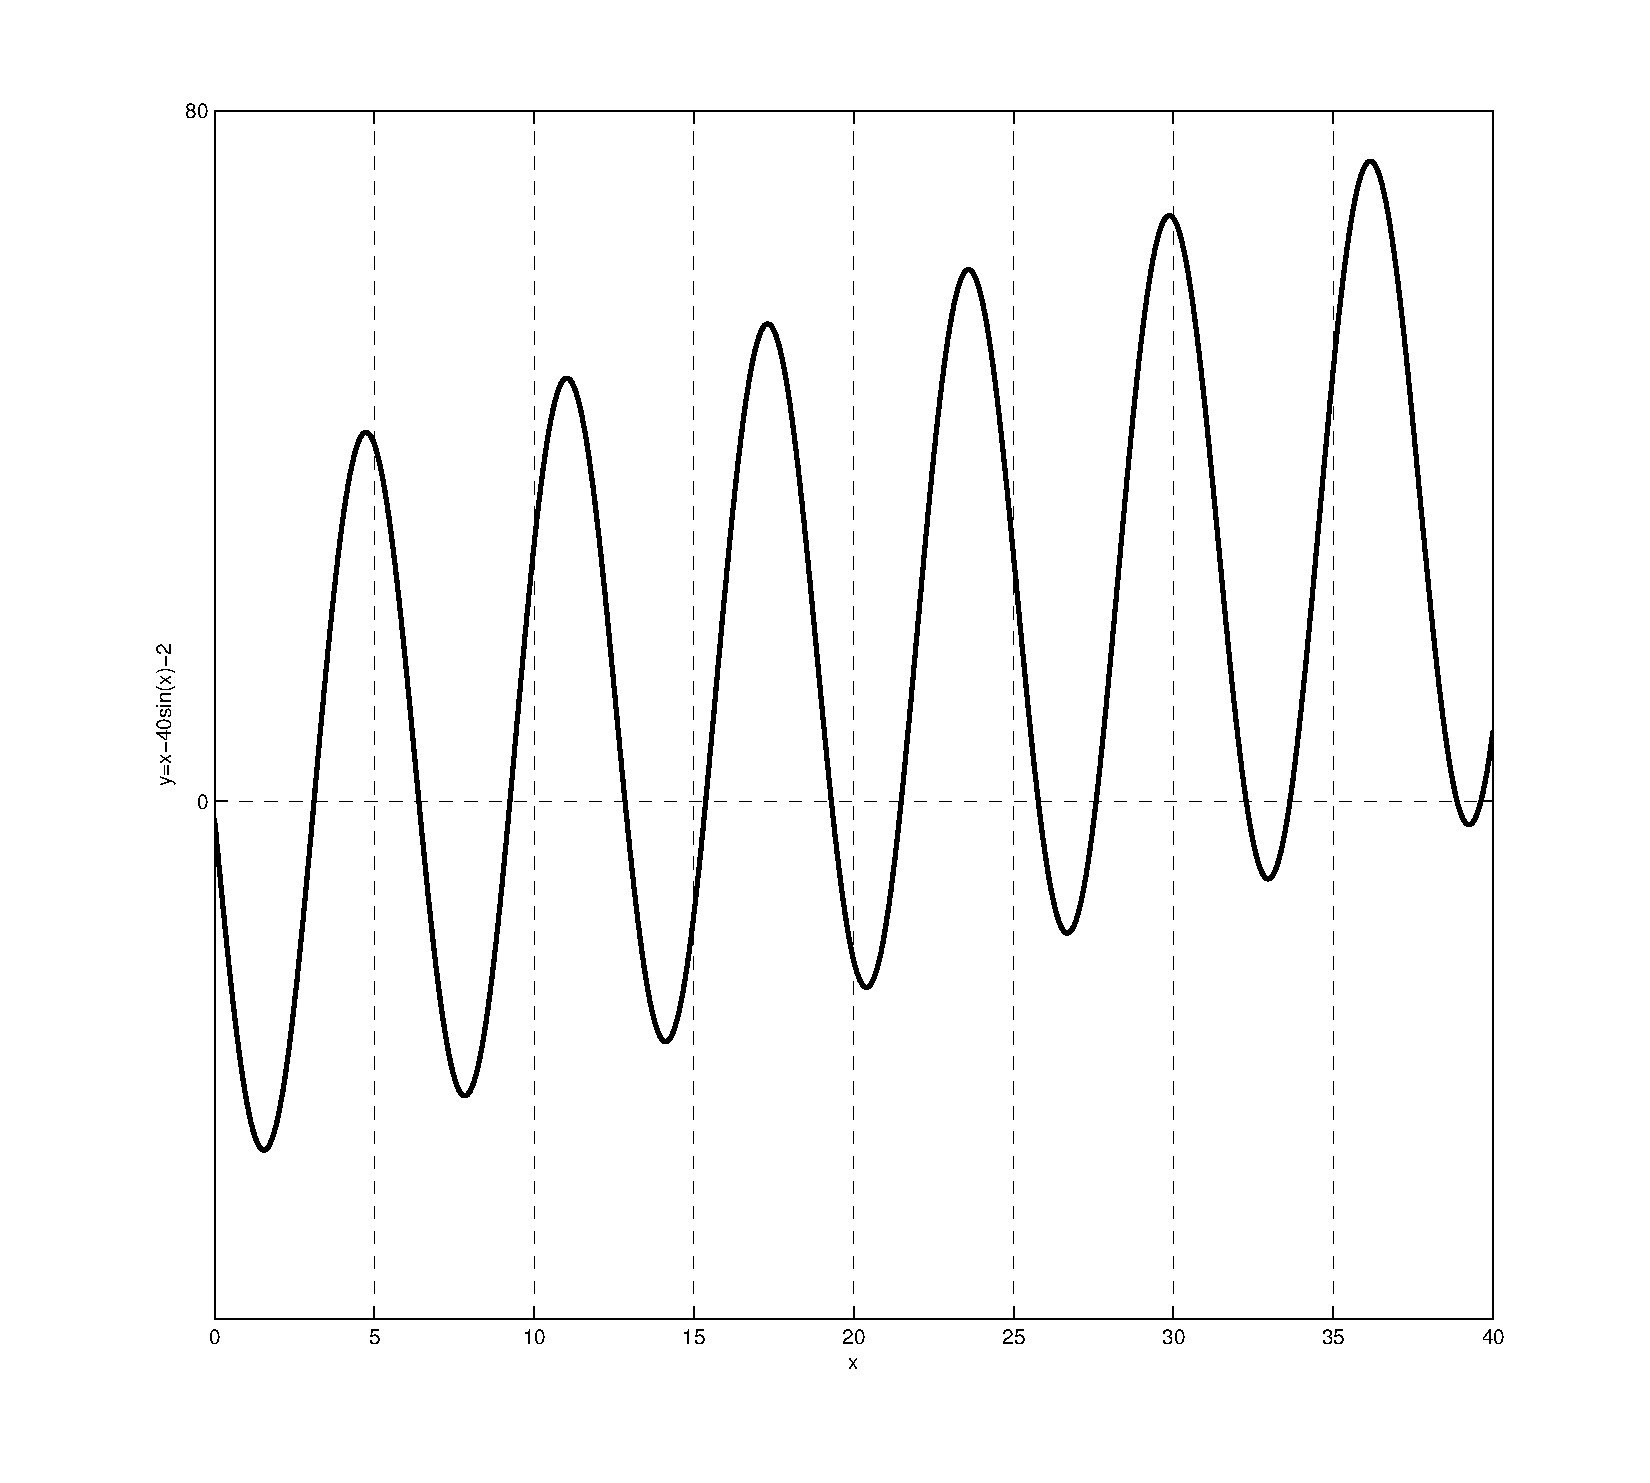
\includegraphics[width=12cm]{kepler.pdf}
	\bicaption{Ejemplo de ecuación de Kepler para $a=40$ y $b=2$.}{ An Example of Kepler's equation is taking $a=40$ and $b=2$.}
	\label{fig:kepler}
\end{figure}
\begin{paracol}{2}

\paragraph*{Métodos iterativos} 
Todos los métodos que se describen en este capítulo, se basan en procedimientos iterativos. La idea es estimar un valor inicial para la raíz $r_0$, y a partir de él ir refinando paso a paso la solución, de modo que el resultado se acerque cada vez más al valor real de la raíz. Cada nueva aproximación a la raíz se obtiene a partir de las aproximaciones anteriores.
\switchcolumn
\paragraph*{Iterative methods} This chapter solely focuses on iterative techniques. These methods begin with an initial guess for the root, denoted as $r_0$, and then gradually refine the solution through a series of iterative steps. With each step, the solution gets closer and closer to the actual value of the root. The successive approximations of the root are carried out based on the previous ones. 
\end{paracol}
\begin{align*}
r_0\ \ \  \rightarrow \  \ r_1  \ \ \rightarrow \ \ r_2 \ \ \rightarrow \cdots \rightarrow \ \ r_k \ \rightarrow \cdots\\
\vert f(r_0)\vert \ge \vert f(r_1)\vert \ge \vert f(r_2)\vert \ge \cdots \ge \vert f(r_k)\vert \ge \cdots
\end{align*}
\begin{paracol}{2}
El proceso que lleva de una solución aproximada a la siguiente se conoce con el nombre de \emph{iteración}. Lo habitual es que en cada iteración se realicen las mismas operaciones matemáticas una y otra vez. 

El proceso se detiene cuando la solución alcanzada se estima lo suficientemente próxima a la solución real como para darla por buena. Para ello, se suele establecer un valor (\emph{tolerancia}) que actúa como criterio de convergencia. De este modo, las iteraciones se repiten hasta que se llega a un valor $r_n$ 	que cumple,
\begin{equation*}
\vert f(r_n) \vert \leq \text(tol)
\end{equation*}

Se dice entonces que el algoritmo empleado para obtener la raíz ha convergido en \emph{n} iteraciones. Por otro lado, es importante señalar que los algoritmos para el cálculo de raíces de una función no siempre convergen. Hay veces en que no es posible aproximarse cada vez más al valor de la raíz bien por la naturaleza de la función o bien por que el algoritmo no es adecuado para obtenerla.
\switchcolumn

Going from one approximate solution to the next is called \emph{iteration}. Usually, the same mathematical operations are repeated in each iteration.

The iterative process comes to a halt when the obtained solution is considered to be close enough to the actual solution to be considered a good approximation. Typically, a value is set as a convergence criterion, known as tolerance. The iterations continue until a value $r_n$ is obtained that satisfies the criterion.
\begin{equation*}
\vert f(r_n) \vert \leq \text(tol)
\end{equation*}

The algorithm used to obtain the root is then said to have converged in \emph{n} iterations. On the other hand, it is important to note that algorithms for calculating the root of a function do not always converge. Sometimes it is not possible to get closer and closer to the value of the root either because of the nature of the function or because the algorithm is not suitable for obtaining it.

\end{paracol}
\begin{paracol}{2}
\paragraph*{Búsqueda local.} Una función puede tener cualquier número de raíces, incluso infinitas, basta pensar por ejemplo en funciones trigonométricas como $\cos(x)$. Una característica importante de los métodos descritos en este capítulo es que solo son capaces de aproximar una raíz. La raíz de la función a la que el método converge depende de el valor inicial $r_0$ con el que se comienza la búsqueda iterativa\footnote{En ocasiones, como veremos más adelante no se suministra al algoritmo un valor inicial, sino un intervalo en el que buscar la raíz}. Por ello reciben el nombre de métodos locales. Si queremos encontrar varias (o todas) las raíces de una determinada función, es preciso emplear el método para cada una de las raíces por separado, cambiando cada vez el punto de partida.
\switchcolumn

\paragraph*{Local search}. A function can have any number of roots, even infinite ones, just think for example of trigonometric functions such as $\cos(x)$. An important feature of the methods described in this chapter is that they are only able to approximate one root. The root of the function to which the method converges depends on the initial value $r_0$ with which the iterative search is started \footnote{Sometimes, as we will see later on, the algorithm is not given an initial value, but an interval in which to search for the root}. This is why they are called local methods. If we want to find several (or all) the roots of a given function, it is necessary to use the method on each of the roots separately, changing the starting point each time.
\end{paracol}

\begin{paracol}{2}
\section{Metodos iterativos locales}
\subsection{Método de la bisección}
\paragraph*{Teorema de Bolzano.}
\begin{quote}
Si una funcion $f(x)$, continua en el intervalo $[a, b]$, cambia de signo en los extremos del intervalo: $f(a)\cdot f(b) \le 0$, debe tener una raíz en el intervalo [a, b]. (figura: \ref{fig:bolzano}) 
\end{quote}

\switchcolumn
\section{Local iterative methods}
\subsection{Bisection Method}
\paragraph*{Bolzano's theorem}
\begin{quote}
    Let $f(x)$ be a continuous function defined in an interval $[a, b]$. Then, if $f(a)\cdot f(b)<0$
(therefore,$f(a)<0$ and $f(b)>0$ or $f(a)>0$ and $f(b)<0$), there exists at least a point inside the interval $c \in [a,b]$ such that $f(c)=0$. (figure: \ref{fig:bolzano})
\end{quote}
\end{paracol}

\begin{figure}[h]
\centering
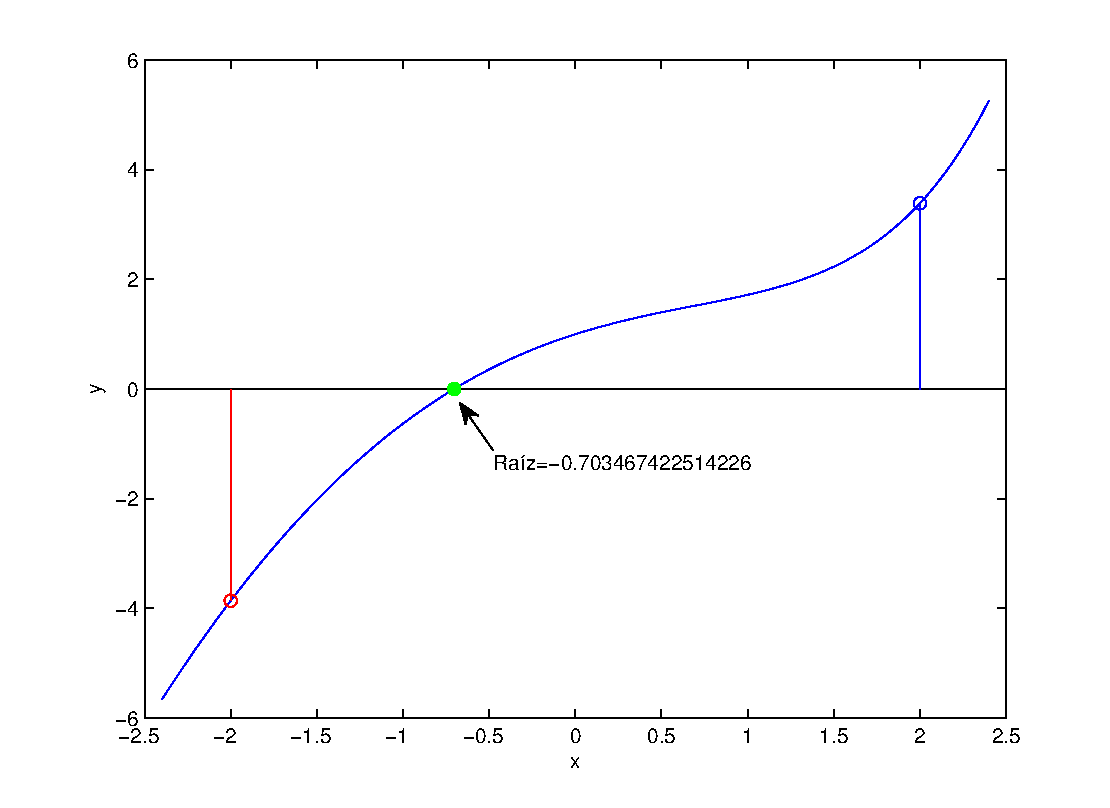
\includegraphics[width=14cm]{bolzano.pdf}
\bicaption{Ilustración del teorema de Bolzano}{Bolzano's theorem.}
\label{fig:bolzano}
\end{figure}

\begin{paracol}{2}

El conocido teorema de Bolzano, suministra el método más sencillo de aproximar la raíz de una función: Se parte de un intervalo inicial en el que se cumpla el teorema; y se va acotando sucesivamente el intervalo que contiene la raíz, reduciéndolo a la mitad en cada iteración, de forma que en cada nuevo intervalo se cumpla siempre el teorema de Bolzano.
\switchcolumn

The well-known Bolzano's theorem provides the simplest method of approximating the root of a function: We start from an initial interval in which the theorem is satisfied; and we successively limit the interval containing the root, reducing it by half in each iteration, so that in each new interval Bolzano's theorem is always satisfied.

\end{paracol}

\begin{figure}[h]
\centering
\begin{tikzpicture}
%\usetikzlibrary{shapes.geometric}
\path (5,0) node(a) [rectangle,draw=blue, very thick,align=center,rounded corners]{Partimos de $[a,b]$\\ con\\ $f(a)\cdot f(b)<0$}
(5,-2) node(b)[rectangle,draw=blue, thick,rounded corners]{Calculamos $c=\frac{a+b}{2}, f(c)$}
(5,-4) node(c)[diamond,aspect=3,draw=red,thick]{es $\vert f(c) \vert \le \text{tol}$?}
(9,-4) node(d)[rectangle,draw=blue,align=center,very thick, rounded corners]{convergencia:\\ terminar}
(5,-6) node(e)[diamond,aspect=3,draw=red,thick]{es $f(a)\cdot f(c) < 0$?}
(9.5,-6) node(f)[rectangle,draw=blue,thick,rounded corners,align=center]{$b=c$\\$f(b)=f(c)$}
(5,-8) node(g)[rectangle,draw=blue,thick,rounded corners,align=center]{$a=c$\\$f(a)=f(c)$};
\draw[blue,-latex](a.south)--(b);
\draw[blue,-latex](b.south)--(c);
\draw[blue,-latex](c.east)--(d);
\draw (7.5,-4)node[above]{Sí};
\draw[blue,-latex](c.south)--(e);
\draw (5,-5)node[right]{No};
\draw[blue,-latex](e.east)--(f);
\draw (7.5,-6)node[above]{Sí};
\draw[blue,-latex](e.south)--(g);
\draw (5,-7.2)node[right]{No};
\draw[blue,-latex](g.south)|-(2,-9)|-(b);
\draw[blue,-latex](f.east)-|(11,-2)--(b);
\end{tikzpicture}
\caption{Diagrama de flujo del método de la bisección}
\label{fig:dfbisec}
\end{figure}


\begin{figure}[h]
\centering
\begin{tikzpicture}
%\usetikzlibrary{shapes.geometric}
\path (5,0) node(a) [rectangle,draw=blue, very thick,align=center,rounded corners]{Begin with $[a,b]$\\ such as\\ $f(a)\cdot f(b)<0$}
(5,-2) node(b)[rectangle,draw=blue, thick,rounded corners]{Compute $c=\frac{a+b}{2}, f(c)$}
(5,-4) node(c)[diamond,aspect=3,draw=red,thick]{is $\vert f(c) \vert \le \text{tol}$?}
(9,-4) node(d)[rectangle,draw=blue,align=center,very thick, rounded corners]{Convergence:\\ finish}
(5,-6) node(e)[diamond,aspect=3,draw=red,thick]{is $f(a)\cdot f(c) < 0$?}
(9.5,-6) node(f)[rectangle,draw=blue,thick,rounded corners,align=center]{$b=c$\\$f(b)=f(c)$}
(5,-8) node(g)[rectangle,draw=blue,thick,rounded corners,align=center]{$a=c$\\$f(a)=f(c)$};
\draw[blue,-latex](a.south)--(b);
\draw[blue,-latex](b.south)--(c);
\draw[blue,-latex](c.east)--(d);
\draw (7.5,-4)node[above]{Yes};
\draw[blue,-latex](c.south)--(e);
\draw (5,-5)node[right]{No};
\draw[blue,-latex](e.east)--(f);
\draw (8,-6)node[above]{Yes};
\draw[blue,-latex](e.south)--(g);
\draw (5,-7.2)node[right]{No};
\draw[blue,-latex](g.south)|-(2,-9)|-(b);
\draw[blue,-latex](f.east)-|(11,-2)--(b);
\end{tikzpicture}
\caption{Flowchart of the bisection method}
\label{fig:dfbisec_eng}
\end{figure}

\begin{paracol}{2}

En la figura \ref{fig:dfbisec} se muestra un diagrama de flujo correspondiente al método de la bisección. El punto de partida es un intervalo $[a,b]$ en el que se cumple el teorema de Bolzano, y que contiene por tanto al menos una raíz. Es interesante hacer notar que el teorema de Bolzano se cumple siempre que la función sea continua en el intervalo $[a,b]$ y existan un número impar de raíces. Por esto es importante realizar cuidadosamente la elección del intervalo $[a,b]$, si hay más de una raíz, el algoritmo puede no converger.

\switchcolumn

Figure \ref{fig:dfbisec_eng} shows a flowchart corresponding to the bisection method. The starting point is an interval $[a,b]$ in which Bolzano's theorem is satisfied, and which therefore contains at least one root. It is interesting to note that Bolzano's theorem is satisfied whenever the function is continuous on the interval $[a,b]$ and there are an odd number of roots. This is why it is important to choose the interval $[a,b]$ carefully. If there is more than one root, the algorithm may not converge.

\switchcolumn
 Una vez que se tiene el intervalo se calcula el punto medio $c$. A continuación se compara el valor que toma la función en $c$, es decir $f(c)$ con la tolerancia. Si el valor es menor que ésta, el algoritmo ha encontrado un valor aproximado de la raíz con la tolerancia requerida, con lo que $c$ es la raíz y no hace falta seguir buscando. Si por el contrario, $f(c)$ está por encima de la tolerancia requerida, comparamos su signo con el que toma la función en uno cualquiera de los extremos del intervalo, En el diagrama de flujo se ha elegido el extremo $a$, pero el algoritmo funcionaría igualmente si eligiéramos $b$. Si el signo de $f(c)$ coincide con el que toma la función en el extremo del intervalo elegido, $c$ sustituye al extremo, (hacemos $a=c$ y $f(a)=f(c)$) si por el contrario el signo es distinto, hacemos que $c$ sustituya al otro extremo del intervalo. (hacemos $b=c$ y $f(b)=f(c)$). Este proceso se repetirá hasta que se cumpla que $f(c)\le \text{tol}$ 

\switchcolumn

 Once we have the interval we calculate the midpoint $c$. The value taken by the function at $c$, i.e. $f(c)$, is then compared with the tolerance. If the value is less than the tolerance, the algorithm has found an approximate value of the root with the required tolerance, so $c$ is the root and no further search is necessary. If, on the other hand, $f(c)$ is above the required tolerance, we compare its sign with the sign of the function at either end of the interval. In the flowchart we have chosen the end $a$, but the algorithm would work equally well if we chose $b$. If the sign of $f(c)$ coincides with the sign that the function takes at the end of the chosen interval, $c$ replaces the end, (we make $a=c$ and $f(a)=f(c)$) if on the contrary the sign is different, we make $c$ replace the other end of the interval (we make $b=c$ and $f(b)=f(c)$). This process will be repeated until $f(c)$ is satisfied. 


\end{paracol} 

\begin{figure}
\centering
\subfigure[intervalo inicial]{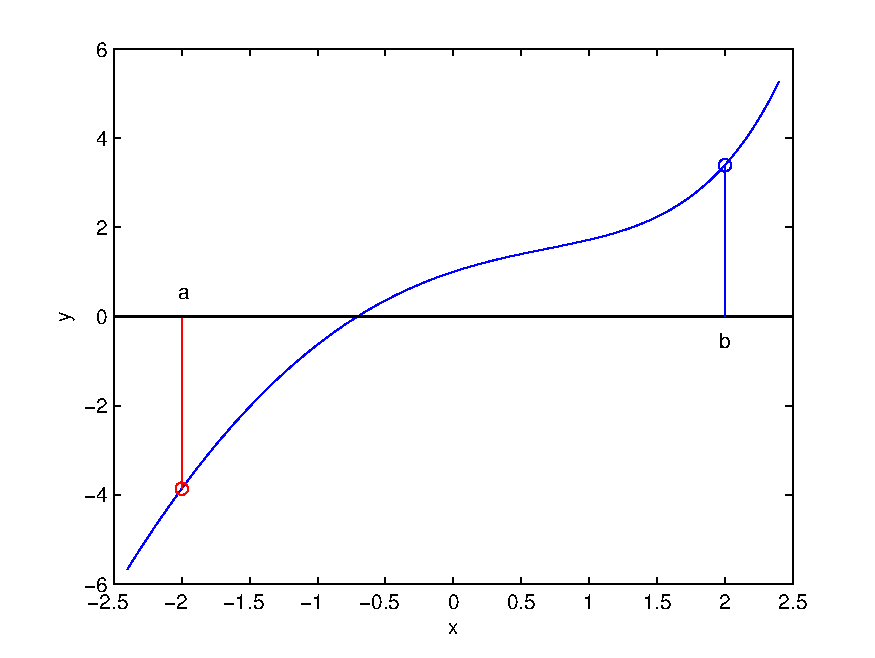
\includegraphics[width=7cm]{rint0.pdf}} \qquad
\subfigure[iteracion 1]{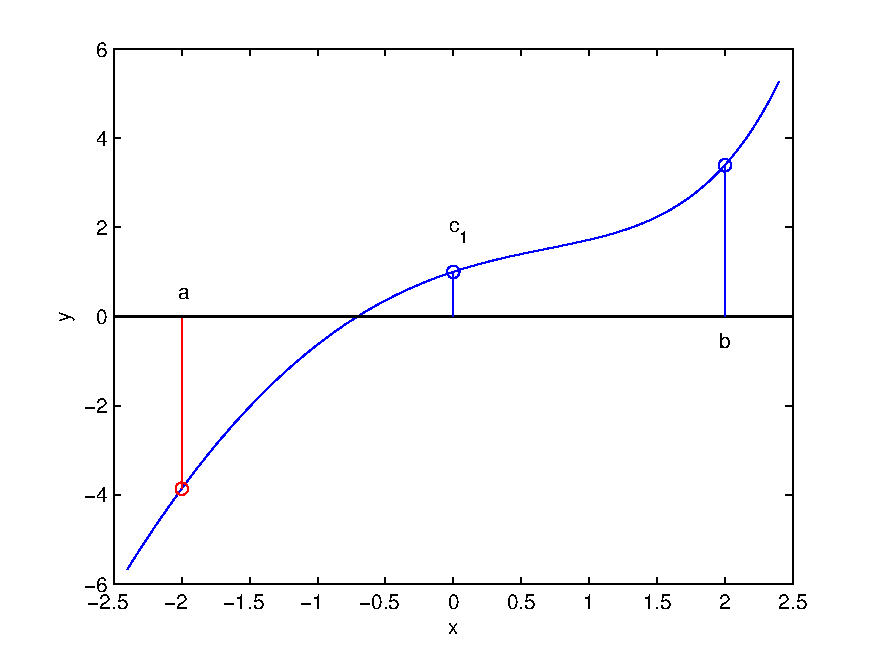
\includegraphics[width=7cm]{rint1.pdf}}\\
\subfigure[iteracion 2]{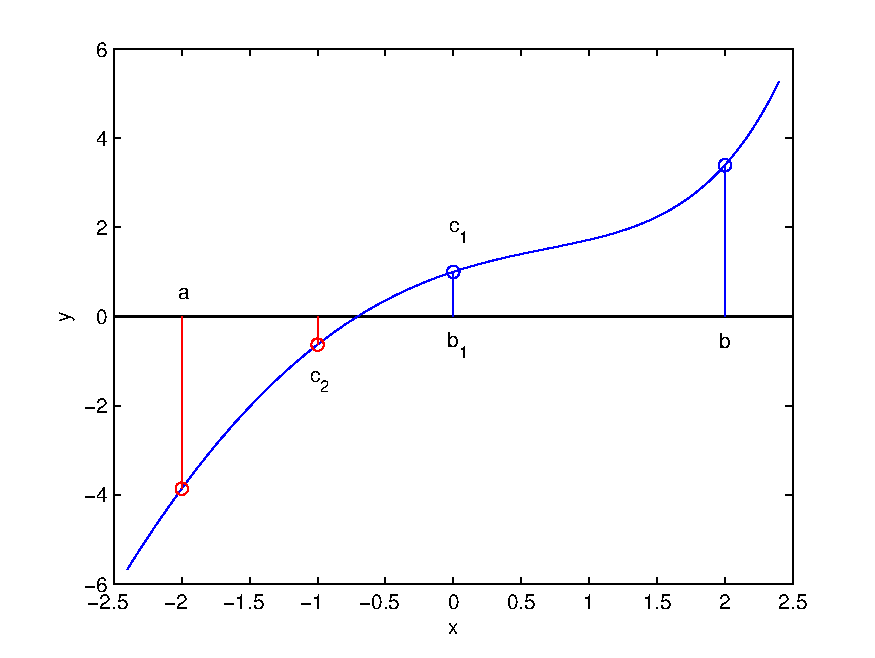
\includegraphics[width=7cm]{rint2.pdf}}\qquad
\subfigure[iteracion 3]{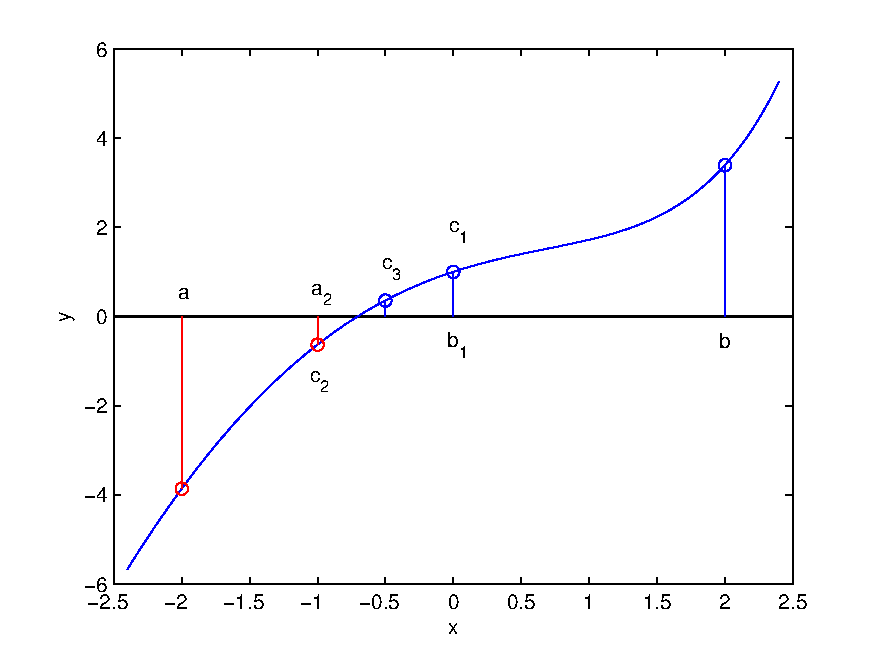
\includegraphics[width=7cm]{rint3.pdf}}\\
\subfigure[iteracion 6: raíz alcanzada]{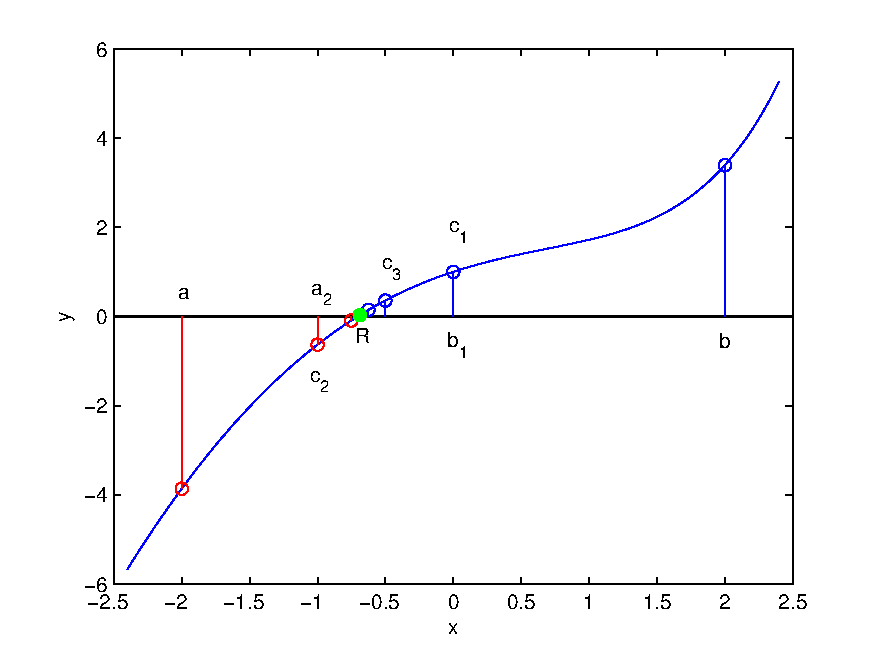
\includegraphics[width=7cm]{rint4.pdf}}

\bicaption{proceso de obtención de la raíz de una función por el método de la bisección.}{process of obtaining the root of a function by the bisection method.}
\label{fig:bisec}
\end{figure}

\begin{paracol}{2}
El proceso se muestra gráficamente en la figura \ref{fig:bisec}, para un caso particular. Se trata de obtener la raíz de la función mostrada en la figura \ref{fig:bolzano}, $f(x)=e^x-x^2$. esta función tiene una única raíz: $r\approx -0.7035$. Para iniciar el algoritmo se ha elegido un intervalo $[a=-2,b=2]$. La figura \ref{fig:bisec}, muestra tres iteraciones sucesivas,y la solución final, que se obtiene al cabo de ocho iteraciones en éste ejemplo, para el que se a empleado una tolerancia $tol=0.01$. En la secuencia de gráficas se puede observar también la evolución del intervalo de búsqueda, $[-2, 2]\rightarrow [-2, 0] \rightarrow [-1, 0] \rightarrow [-1, -0.5] \cdots$; así como el cambio alternativo del límite derecho o izquierdo, para asegurar que la raíz queda siempre dentro de los sucesivos intervalos de búsqueda obtenidos. 

\switchcolumn

The process is shown graphically in figure \ref{fig:bisec}, for a particular case. This is to obtain the root of the function shown in figure \ref{fig:bolzano}, $f(x)=e^x-x^2$. This function has a single root: $r\approx -0.7035$. To start the algorithm, an interval $[a=-2,b=2]$ has been chosen. Figure \ref{fig:bisec}, shows three successive iterations, and the final solution, which is obtained after eight iterations in this example, for which a tolerance $tol=0.01$ has been used. The sequence of graphs also shows the evolution of the search interval, $[-2, 2]\rightarrow [-2, 0] \rightarrow [-1, 0] \rightarrow [-1, -0.5] \cdots$; as well as the alternative change of the right or left limit, to ensure that the root is always within the successive search intervals obtained. 



\switchcolumn


\subsection{Método de interpolación lineal o (\emph{Regula falsi})}
Este método supone una mejora del anterior ya que, en general,  converge más rápidamente. La idea es modificar el modo en que calculamos el punto $c$. En el caso del método de la bisección el criterio consistía en ir tomando en cada iteración el punto medio del intervalo que contiene la raíz. El método de interpolación lineal, elige como punto $c$ el punto de corte con el eje x, de la recta que pasa por los puntos $\left(a,f(a)\right)$ y $\left(b,f(b)\right)$. Es decir la recta que corta a la función $f(x)$ en ambos límites del intevalo que contiene a la raíz buscada. La recta que pasa por ambos puntos puede construirse a partir de ellos como,

\begin{equation*}
y=\frac{f(a)-f(b)}{a-b}\cdot(x-b)+f(b)
\end{equation*}
el punto de corte con el eje $x$, que será el valor que tomaremos para $c$, se obtiene cuando $y=0$,
\begin{equation*}
0=\frac{f(a)-f(b)}{a-b}\cdot(x-b)+f(b)
\end{equation*}

y despejando $c\equiv x$ en la ecuación anterior obtenemos,
\begin{equation*}
c=b-\frac{f(b)}{f(b)-f(a)}\cdot(b-a)
\end{equation*}

\switchcolumn

\subsection{False position method or (\emph{Regula falsi})}

This method is an improvement on the previous one as it converges more quickly in general. The idea is to modify the way in which we calculate the point $c$. In the case of the bisection method, the criterion consisted of taking the midpoint of the interval containing the root at each iteration. The linear interpolation method chooses as point $c$ the point of intersection with the x-axis of the straight line that passes through the points $\left(a,f(a)\right)$ and $\left(b,f(b)\right)$. That is, the line that cuts the function $f(x)$ at both limits of the interval containing the root we are looking for. The line through both points can be constructed from them as,

\begin{equation*}
y=\frac{f(a)-f(b)}{a-b}\cdot(x-b)+f(b)
\end{equation*}

The intersection point with the x-axis, will be the value for $c$, is obtained when $y=0$,

\begin{equation*}
0=\frac{f(a)-f(b)}{a-b}\cdot(x-b)+f(b)
\end{equation*}

and replacing $cequiv x$ in the above equation, we get

\begin{equation*}
c=b-\frac{f(b)}{f(b)-f(a)}\cdot(b-a)
\end{equation*}

\switchcolumn
La figura \ref{fig:regulaf} muestra  gráficamente la posición del punto $c$ obtenido mediante el método de interpolación.

\switchcolumn
Figure \ref{fig:regulaf} shows the position of point $c$ computed with this method.
\end{paracol}

\begin{figure}[h]
\centering
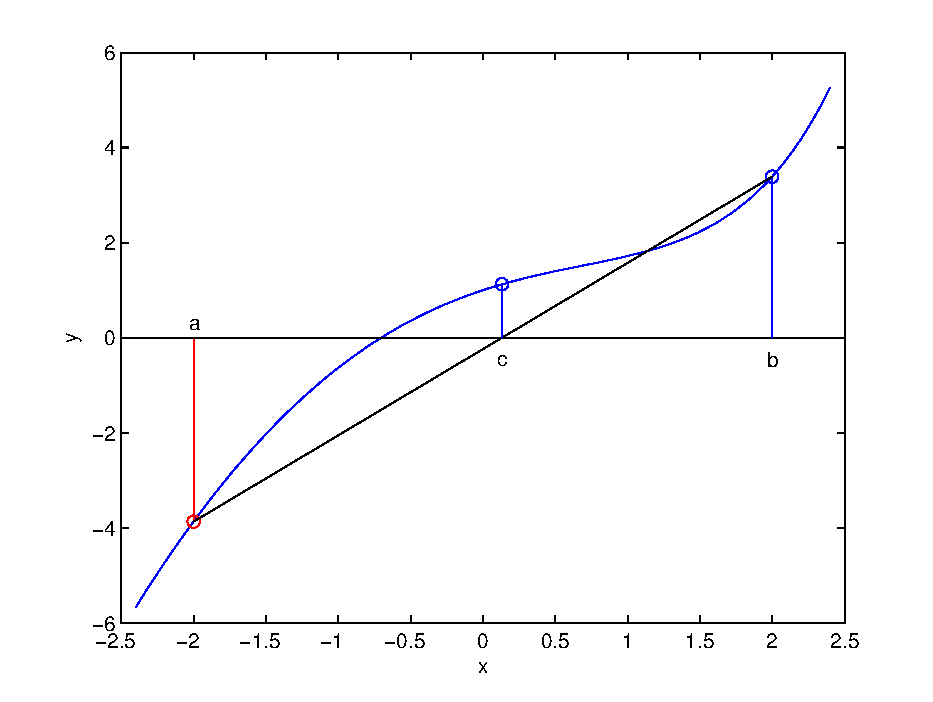
\includegraphics[width=14cm]{rinter00.pdf}

\bicaption{Obtención de la recta que une los extremos de un intervalo $[a,b]$  que contiene una raíz de la función}{Obtaining the line joining the extremes of an interval $[a,b]$ containing a root of the function}
\label{fig:regulaf}
\end{figure}

\begin{paracol}{2}
    Por lo demás, el procedimiento es el mismo que en el caso del método de la bisección. Se empieza con un intervalo $[a,b]$ que  contenga una raíz, se obtiene el punto $c$ por el procedimiento descrito y se intercambia $c$ con el extremo del intervalo cuya imagen $f(a)$ o $f(b)$ tenga el mismo signo que $f(c)$ el procedimiento se repite iterativamente hasta que f(c) sea menor que el valor de tolerancia preestablecido. 

    \switchcolumn
    Otherwise, the procedure is the same as in the case of the bisection method. We start with an interval $[a,b]$ containing a root, obtain the point $c$ by the procedure described above and exchange $c$ with the end of the interval whose image $f(a)$ or $f(b)$ has the same sign as $f(c)$. The procedure is repeated iteratively until $f(c)$ is less than the preset tolerance value. 
    
\end{paracol}


\begin{figure}[h]
\centering
\begin{tikzpicture}
%\usetikzlibrary{shapes.geometric}
\path (5,0) node(a) [rectangle,draw=blue, very thick,align=center,rounded corners]{Partimos de $[a,b]$\\ con\\ $f(a)\cdot f(b)<0$}
(5,-2) node(b)[rectangle,draw=blue, thick,rounded corners,align=center]{Calculamos\\ $c=b-\frac{f(b)}{f(b)-f(a)}\cdot(b-a), f(c)$}
(5,-4) node(c)[diamond,aspect=3,draw=red,thick]{es $\vert f(c) \vert \le \text{tol}$?}
(9,-4) node(d)[rectangle,draw=blue,align=center,very thick, rounded corners]{convergencia:\\ terminar}
(5,-6) node(e)[diamond,aspect=3,draw=red,thick]{es $f(a)\cdot f(c) < 0$?}
(9.5,-6) node(f)[rectangle,draw=blue,thick,rounded corners,align=center]{$b=c$\\$f(b)=f(c)$}
(5,-8) node(g)[rectangle,draw=blue,thick,rounded corners,align=center]{$a=c$\\$f(a)=f(c)$};
\draw[blue,-latex](a.south)--(b);
\draw[blue,-latex](b.south)--(c);
\draw[blue,-latex](c.east)--(d);
\draw (7.5,-4)node[above]{Sí};
\draw[blue,-latex](c.south)--(e);
\draw (5,-5)node[right]{No};
\draw[blue,-latex](e.east)--(f);
\draw (8,-6)node[above]{Sí};
\draw[blue,-latex](e.south)--(g);
\draw (5,-7.2)node[right]{No};
\draw[blue,-latex](g.south)|-(2,-9)|-(b);
\draw[blue,-latex](f.east)-|(11,-2)--(b);
\end{tikzpicture}
\caption{Diagrama de flujo del método de interpolación lineal}
\label{fig:regula}
\end{figure}



\begin{figure}[h]
\centering
\begin{tikzpicture}
%\usetikzlibrary{shapes.geometric}
\path (5,0) node(a) [rectangle,draw=blue, very thick,align=center,rounded corners]{Begin with $[a,b]$\\ being\\ $f(a)\cdot f(b)<0$}
(5,-2) node(b)[rectangle,draw=blue, thick,rounded corners,align=center]{Compute\\ $c=b-\frac{f(b)}{f(b)-f(a)}\cdot(b-a), f(c)$}
(5,-4) node(c)[diamond,aspect=3,draw=red,thick]{is $\vert f(c) \vert \le \text{tol}$?}
(9,-4) node(d)[rectangle,draw=blue,align=center,very thick, rounded corners]{It converges:\\ finish}
(5,-6) node(e)[diamond,aspect=3,draw=red,thick]{is $f(a)\cdot f(c) < 0$?}
(9.5,-6) node(f)[rectangle,draw=blue,thick,rounded corners,align=center]{$b=c$\\$f(b)=f(c)$}
(5,-8) node(g)[rectangle,draw=blue,thick,rounded corners,align=center]{$a=c$\\$f(a)=f(c)$};
\draw[blue,-latex](a.south)--(b);
\draw[blue,-latex](b.south)--(c);
\draw[blue,-latex](c.east)--(d);
\draw (7.5,-4)node[above]{Yes};
\draw[blue,-latex](c.south)--(e);
\draw (5,-5)node[right]{No};
\draw[blue,-latex](e.east)--(f);
\draw (8,-6)node[above]{Yes};
\draw[blue,-latex](e.south)--(g);
\draw (5,-7.2)node[right]{No};
\draw[blue,-latex](g.south)|-(2,-9)|-(b);
\draw[blue,-latex](f.east)-|(11,-2)--(b);
\end{tikzpicture}
\caption{Flowchart of false position method}
\label{fig:regula_eng}
\end{figure}

\begin{paracol}{2}
En la figura \ref{fig:regula} se muestra el diagrama de flujo para el método de interpolación lineal. Como puede verse, es idéntico al de la bisección excepto en el paso en que se obtiene el valor de $c$, donde se ha sustituido el cálculo del punto medio del intervalo de búsqueda, por el cálculo del punto de corte con el eje de abscisas  de la recta que une los extremos del intervalo.

\switchcolumn
The flowchart for the false position method is shown in figure \ref{fig:regula_eng}. As can be seen, it is identical to the bisection method except in the step where the value of $c$ is obtained, where the calculation of the midpoint of the search interval has been replaced by the calculation of the point of intersection with the abscissa axis of the straight line joining the ends of the interval.
\switchcolumn

La figura \ref{fig:iterr2} Muestra gráficamente el proceso iterativo seguido para obtener la raíz de una función en un intervalo mediante el método de interpolación lineal. Se ha empleado la misma función y el mismo intervalo inicial que en el caso de la bisección. 
\switchcolumn

Figure \ref{fig:iterr2} shows graphically the iterative process followed to obtain the root of a function in an interval by means of the false position method. The same function and the same initial interval have been used as in the case of bisection. 
\switchcolumn

Es fácil ver, sin embargo, que los puntos intermedios que obtiene el algoritmo hasta converger a la raíz son distintos. De hecho, el algoritmo emplea ahora tan solo siete iteraciones para obtener la raíz, empleando el mismo valor para la tolerancia, 0.01, que se empleó en el método de la bisección.
\switchcolumn


It is easy to see, however, that the intermediate points that the algorithm obtains until converging to the root are different. In fact, the algorithm now uses only seven iterations to obtain the root, using the same value for the tolerance, $0.01$, as was used in the bisection method.
\end{paracol}

\begin{paracol}{2}

Una observación final, se ha dicho al principio que éste método supone una mejora al método anterior de la bisección. Esto no siempre es cierto. El método de la bisección tiene una tasa de convergencia constante, cada iteración divide el espacio de búsqueda por la mitad. Sin embargo la convergencia del método de interpolación  lineal depende de la función $f(x)$ y de la posición relativa de los puntos iniciales $(a, f(a))$  y $(b, f(b))$ con respecto al la raíz. Por esto no es siempre cierto que converja más rápido que el método de  la bisección. Por otro lado, el cálculo de los sucesivos valores del punto $c$, requiere más operaciones aritméticas en el método de interpolación, con lo que cada iteración resulta más lenta que en el caso de la bisección.

\switchcolumn

One final remark, it was said at the beginning that this method is an improvement on the previous method of bisection. This is not always true. The bisection method has a constant convergence rate, each iteration halving the search space. However, the convergence of the false position method depends on the function $f(x)$ and the relative position of the initial points $(a, f(a))$ and $(b, f(b))$ with respect to the root. This is why it is not always true that it converges faster than the bisection method. On the other hand, the calculation of the successive values of the point $c$ requires more arithmetic operations in the false position method, making each iteration slower than in the case of bisection.

\end{paracol}

\begin{figure}
\centering
\subfigure[intervalo inicial]{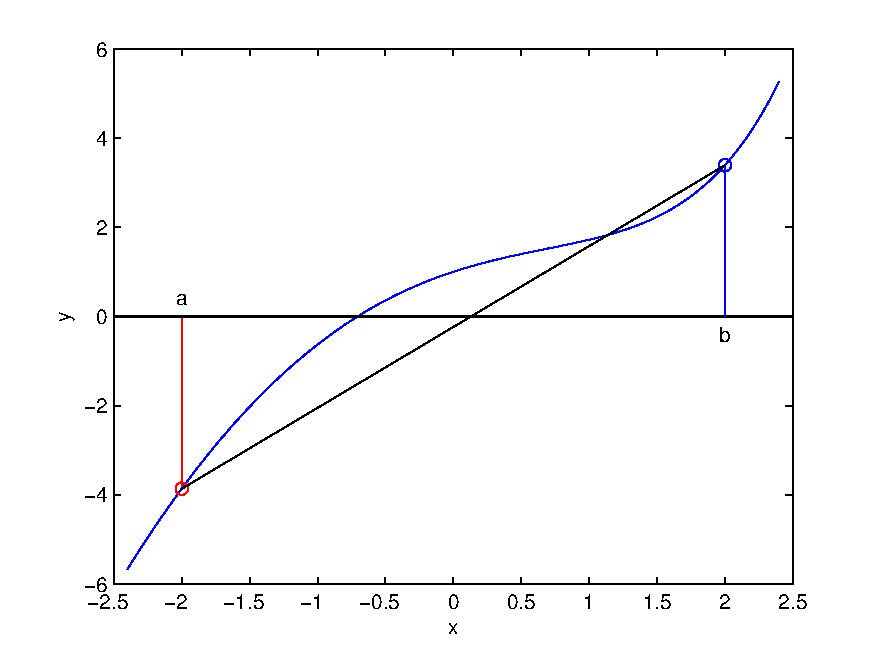
\includegraphics[width=7cm]{rinter0.pdf}} \qquad
\subfigure[iteracion 1]{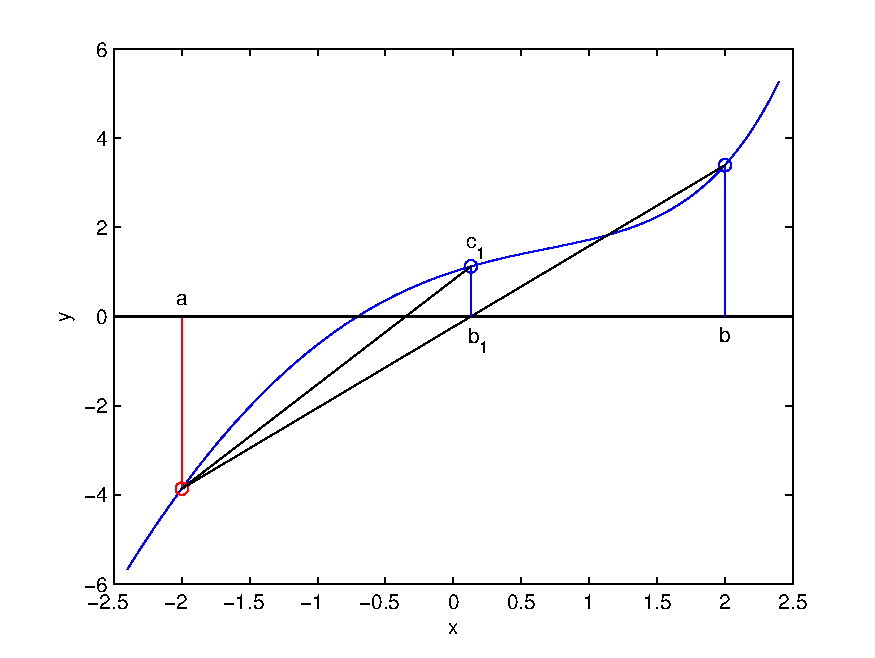
\includegraphics[width=7cm]{rinter1.pdf}}\\
\subfigure[iteracion 2]{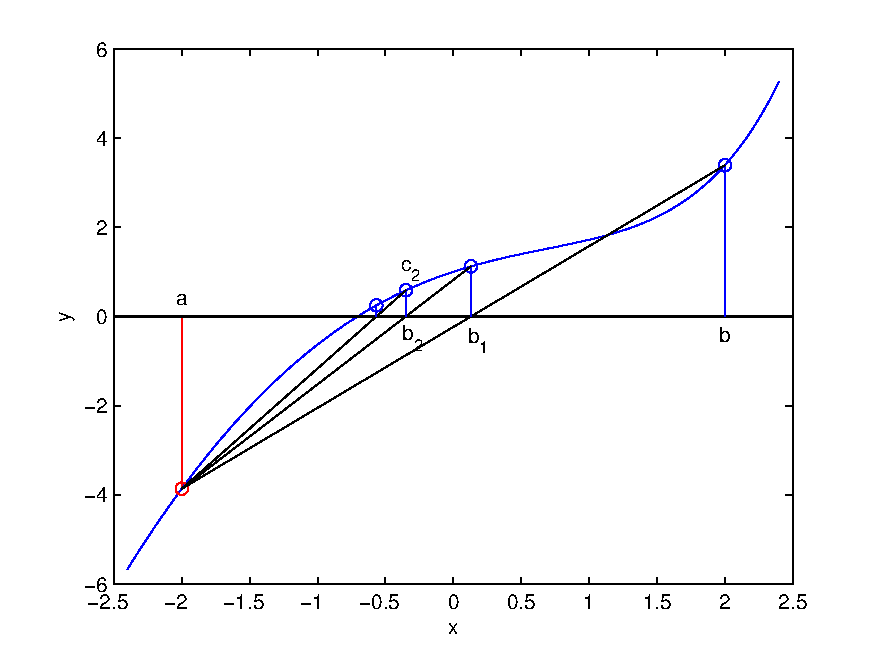
\includegraphics[width=7cm]{rinter2.pdf}}\qquad
\subfigure[iteracion 3]{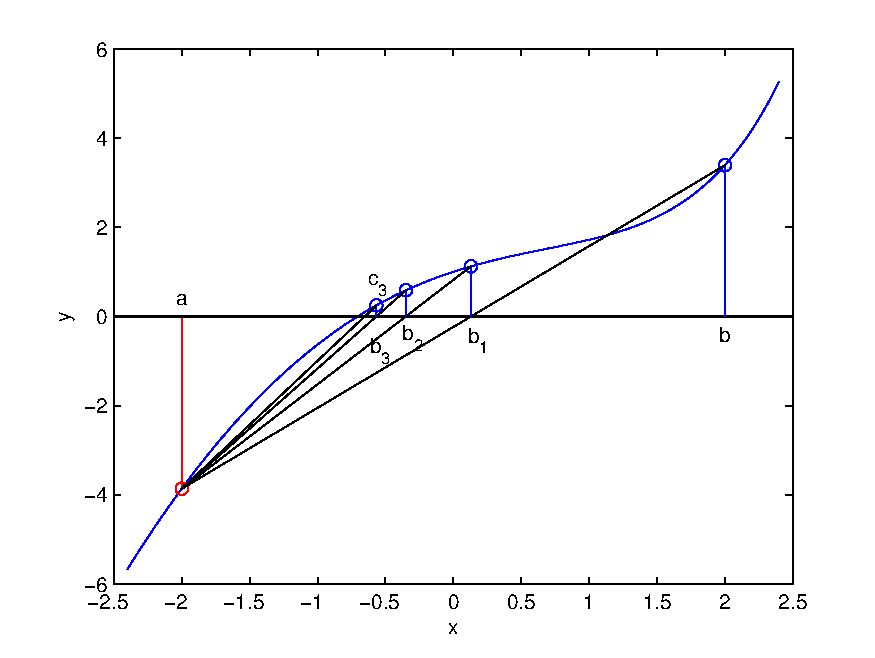
\includegraphics[width=7cm]{rinter3.pdf}}\\
\subfigure[iteracion 6: raíz alcanzada]{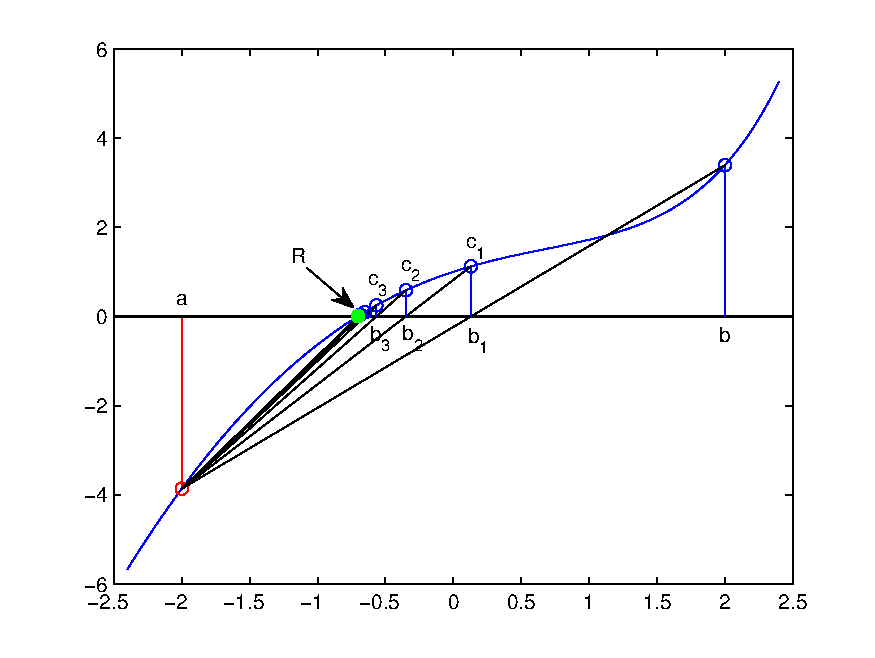
\includegraphics[width=7cm]{rinter4.pdf}}

\bicaption{Proceso de obtención de la raíz de una función por el método de interpolación lineal}{Process of obtaining the root of a function by the method of linear interpolation}\label{fig:iterr2}
\end{figure}

\begin{paracol}{2}
\subsection{Método de Newton-Raphson}
El método de Newton se basa en la expansión de una función $f(x)$ en serie de Taylor en el entorno de un punto $x_0$,

\switchcolumn
\subsection{Newton-Raphson method}
Newton's method is based on the expansion of a Taylor series function $f(x)$ around a point $x_0$,
\end{paracol}
\begin{equation*}
f(x)\approx f(x_0)+f'(x_0)(x-x_0)+\frac{1}{2}f''(x_0)(x-x_0)^2+\cdots+\frac{1}{n!}f^{(n)}(x_0)(x-x_0)^n+\cdots
\end{equation*}

\begin{paracol}{2}
 Pertenece a una familia de métodos ampliamente empleados en cálculo numérico. La idea en el caso del método de Newton es aproximar la función para la que se desea obtener la raíz, mediante el primer término de la serie de Taylor. Es decir aproximar localmente $f(x)$, en el entorno de $x_0$ por la recta,
\begin{equation*}
 f(x_0)+f'(x_0)(x-x_0)
\end{equation*}

\switchcolumn

 It belongs to a family of methods widely used in numerical calculus. The idea in the case of Newton's method is to approximate the function for which one wishes to obtain the root, by means of the first term of Taylor's series. That is to say, to approximate locally $f(x)$, in the environment of $x_0$ by the straight line,
\begin{equation*}
 f(x_0)+f'(x_0)(x-x_0)
\end{equation*}
\end{paracol}

\begin{figure}[h]
\centering
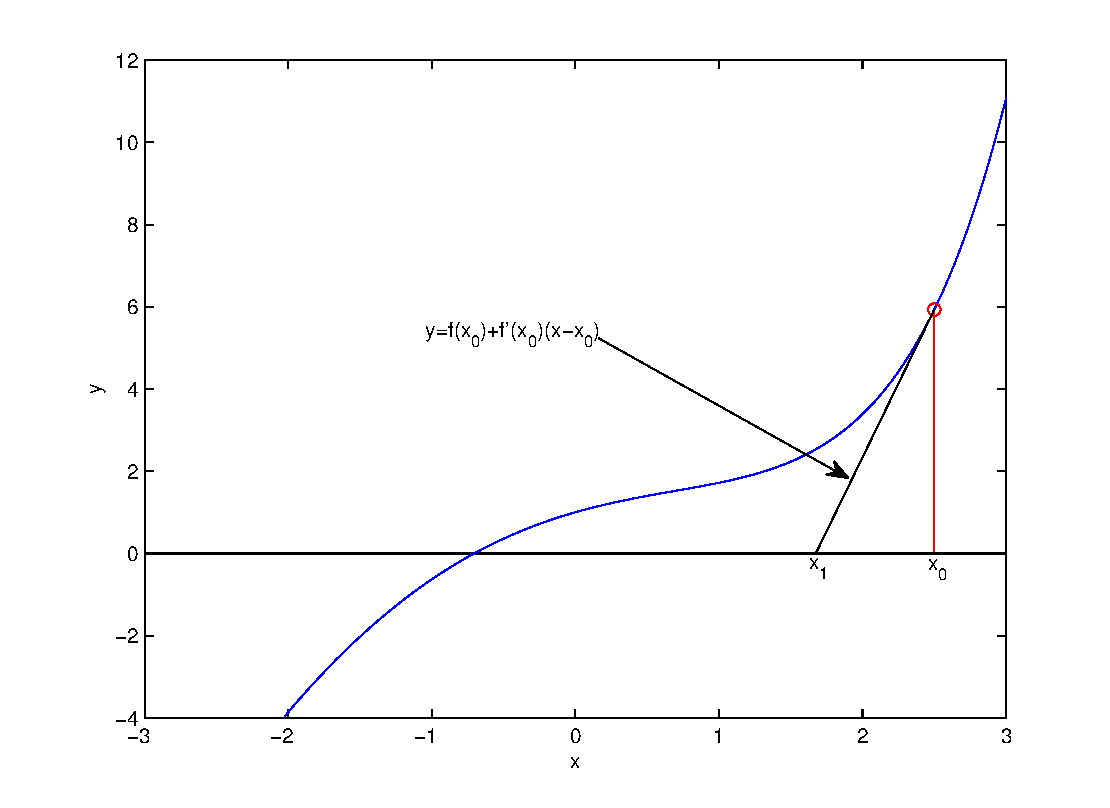
\includegraphics[width=14cm]{newt0.pdf}[h]
\bicaption{Recta tangente a la función $f(x)$ en el punto $x_0$}{Tangent line to the function $f(x)$ at the point $x_0$.}
\label{fig:newton1}
\end{figure}

\begin{paracol}{2}
Esta recta, es precisamente la recta tangente a la curva $f(x)$ en el punto $x_0$ (figura \ref{fig:newton1})

El método consiste en obtener el corte de esta recta tangente con el eje de abscisas,
\begin{equation*}
0= f(x_0)+f'(x_0)(x-x_0)
\end{equation*}

y despejando x,

\begin{equation*}
x=x_0-\frac{f(x_0)}{f'(x_0)}
\end{equation*}

\switchcolumn
This line is precisely the tangent line to the curve $f(x)$ at the point $x_0$ (figure \ref{fig:newton1}).

The method consists of obtaining the intersection of this tangent line with the abscissa axis,
\begin{equation*}
0= f(x_0)+f'(x_0)(x-x_0)
\end{equation*}

and obtaining x,

\begin{equation*}
x=x_0-\frac{f(x_0)}{f'(x_0)}
\end{equation*}

\switchcolumn
A continuación se evalúa la función en el punto obtenido $x\rightarrow f(x)$. Como en los métodos anteriores, se compara el valor de $f(x)$ con una cierta tolerancia preestablecida. Si es menor, el valor de $x$ se toma como raíz de la función. Si no, se vuelve aplicar el algoritmo, empleando ahora el valor de x que acabamos de obtener como punto de partida. Cada cálculo constituye una nueva iteración y los sucesivos valores obtenidos para $x$, convergen a la raíz,

\switchcolumn

Next, the function is evaluated at the point obtained $xrightarrow f(x)$. As in the previous methods, the value of $f(x)$ is compared with a certain pre-set tolerance. If it is smaller, the value of $x$ is taken as the root of the function. If not, the algorithm is applied again, now using the value of x just obtained as the starting point. Each calculation constitutes a new iteration and the successive values obtained for $x$ converge to the root,

\end{paracol}

\begin{equation*}
x_0\rightarrow x_1=x_0-\frac{f(x_0)}{f'(x_0)}\rightarrow x_2=x_1-\frac{f(x_1)}{f'(x_1)}\rightarrow  \cdots \rightarrow x_n=x_{n-1}-\frac{f(x_{n-1})}{f'(x_{n-1})}\rightarrow \cdots
\end{equation*}


\begin{figure}[h]
\centering
\begin{tikzpicture}
%\usetikzlibrary{shapes.geometric}
\path (5,0) node(a) [rectangle,draw=blue, very thick,align=center,rounded corners]{Partimos de un punto inicial $x_0$}
(5,-2) node(b)[rectangle,draw=blue, thick,rounded corners,align=center]{Calculamos\\ $x=x_0-\frac{f(x_0)}{f'(x_0)}, f(x)$}
(5,-4) node(c)[diamond,aspect=3,draw=red,thick]{es $\vert f(x) \vert \le \text{tol}$?}
(9,-4) node(d)[rectangle,draw=blue,align=center,very thick, rounded corners]{convergencia:\\ terminar}
(5,-6) node(g)[rectangle,draw=blue,thick,rounded corners,align=center]{$x_0=x$};
\draw[blue,-latex](a.south)--(b);
\draw[blue,-latex](b.south)--(c);
\draw[blue,-latex](c.east)--(d);
\draw (7.5,-4)node[above]{Sí};
\draw[blue,-latex](c.south)--(g);
\draw (5,-5)node[right]{No};
\draw[blue,-latex](g.south)|-(2,-7)|-(b);

\end{tikzpicture}
\caption{Diagrama de flujo del método de Newton-Raphson}
\label{fig:newton}
\end{figure}

\begin{figure}[h]
\centering
\begin{tikzpicture}
%\usetikzlibrary{shapes.geometric}
\path (5,0) node(a) [rectangle,draw=blue, very thick,align=center,rounded corners]{Initial point $x_0$}
(5,-2) node(b)[rectangle,draw=blue, thick,rounded corners,align=center]{Compute\\ $x=x_0-\frac{f(x_0)}{f'(x_0)}, f(x)$}
(5,-4) node(c)[diamond,aspect=3,draw=red,thick]{is $\vert f(x) \vert \le \text{tol}$?}
(9,-4) node(d)[rectangle,draw=blue,align=center,very thick, rounded corners]{it converges:\\ finish}
(5,-6) node(g)[rectangle,draw=blue,thick,rounded corners,align=center]{$x_0=x$};
\draw[blue,-latex](a.south)--(b);
\draw[blue,-latex](b.south)--(c);
\draw[blue,-latex](c.east)--(d);
\draw (7.5,-4)node[above]{Yes};
\draw[blue,-latex](c.south)--(g);
\draw (5,-5)node[right]{No};
\draw[blue,-latex](g.south)|-(2,-7)|-(b);

\end{tikzpicture}
\caption{Flowchart of Newton-Raphson method}
\label{fig:newton_eng}
\end{figure}

\begin{paracol}{2}

La figura \ref{fig:newton} muestra un diagrama de flujo correspondiente al método de Newton. Si se compara con los diagramas de flujo de los algoritmos anteriores, el algoritmo de Newton resulta algo más simple de implementar. Sin embargo es preciso evaluar en cada iteración el valor de la función y el de su derivada. 

\switchcolumn

Figure \ref{fig:newton_eng} shows a flowchart for Newton's method. Compared to the flowcharts of the previous algorithms, Newton's algorithm is somewhat simpler to implement. However, the value of the function and its derivative must be evaluated at each iteration. 

\switchcolumn

El cálculo de la derivada, es el punto débil de este algoritmo, ya que para valores $x_0$ próximos a un mínimo o máximo local obtendremos valores de la derivada próximos a cero, lo que puede causar un error de desbordamiento al calcular el punto de corte de la recta tangente con el eje de abscisas o hacer que el algoritmo converja a una raíz alejada del punto inicial de búsqueda.
 
\switchcolumn

The calculation of the derivative is the weak point of this algorithm, since for values $x_0$ close to a local minimum or maximum we will obtain values of the derivative close to zero, which may cause an overflow error when calculating the point of intersection of the tangent line with the abscissa axis or cause the algorithm to converge to a root far from the initial search point.

\end{paracol}
\newpage
\begin{figure}

\centering
\subfigure[intervalo inicial]{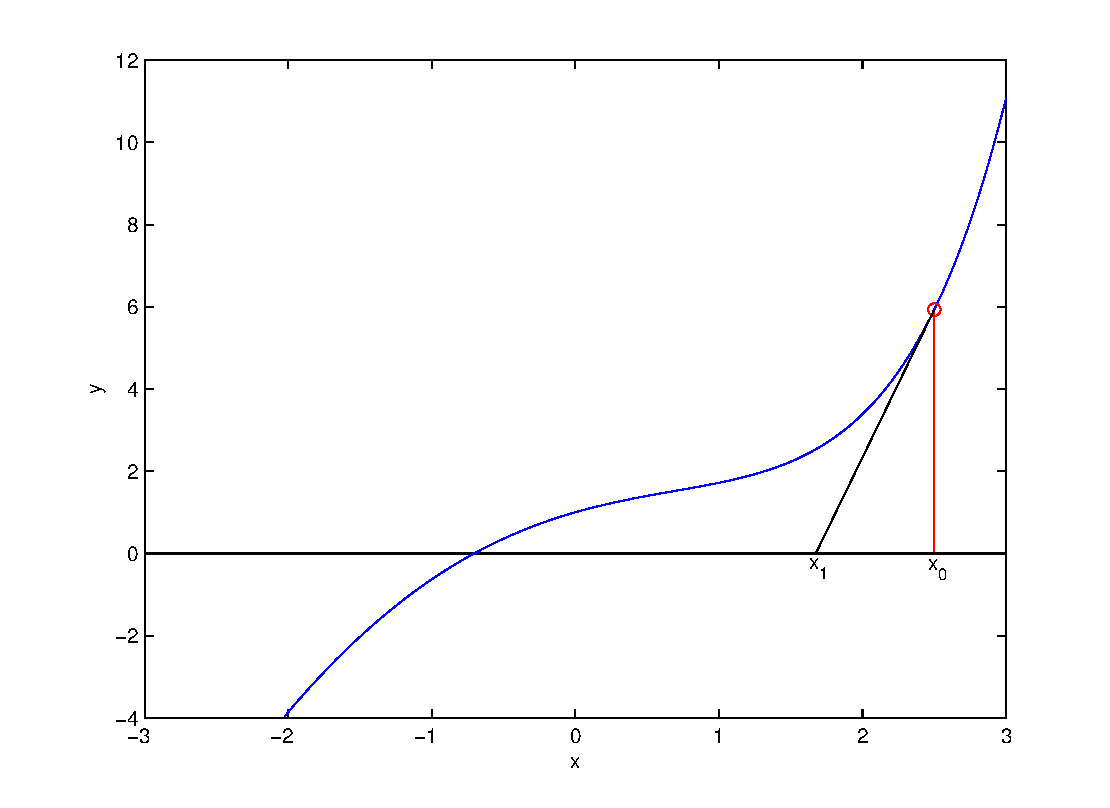
\includegraphics[width=7cm]{newt01.pdf}} \qquad
\subfigure[iteracion 1]{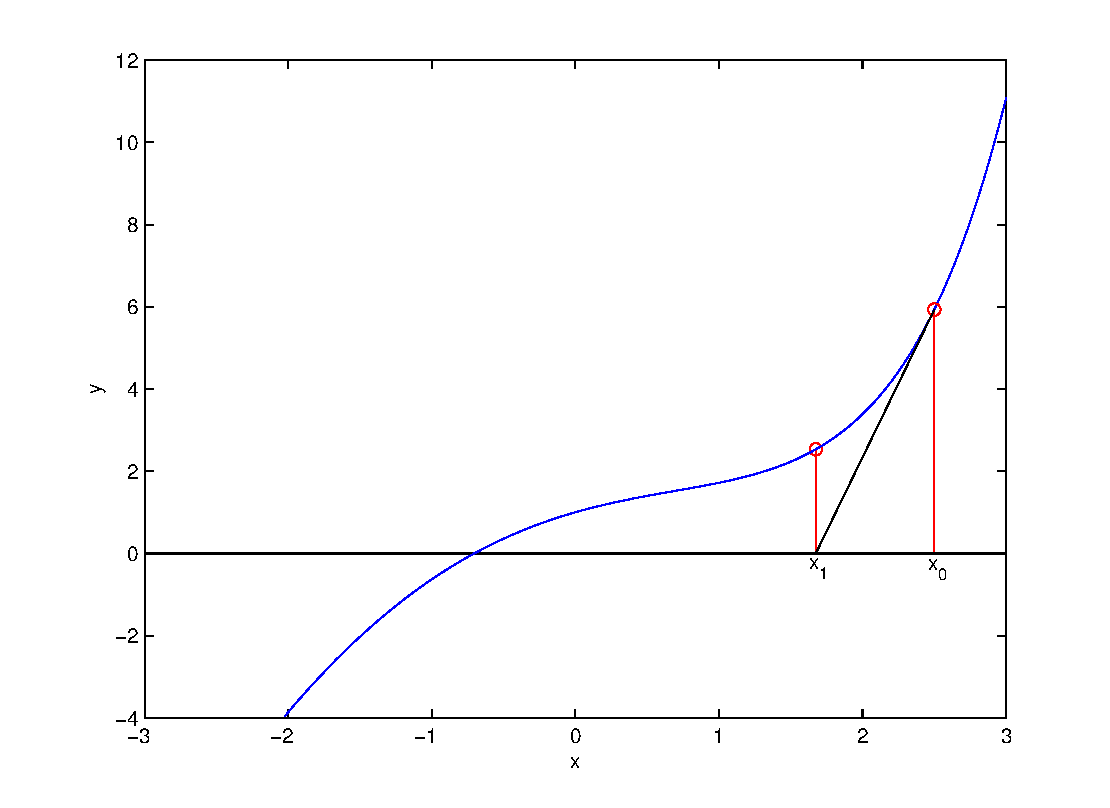
\includegraphics[width=7cm]{newt02.pdf}}\\
\subfigure[iteracion 2]{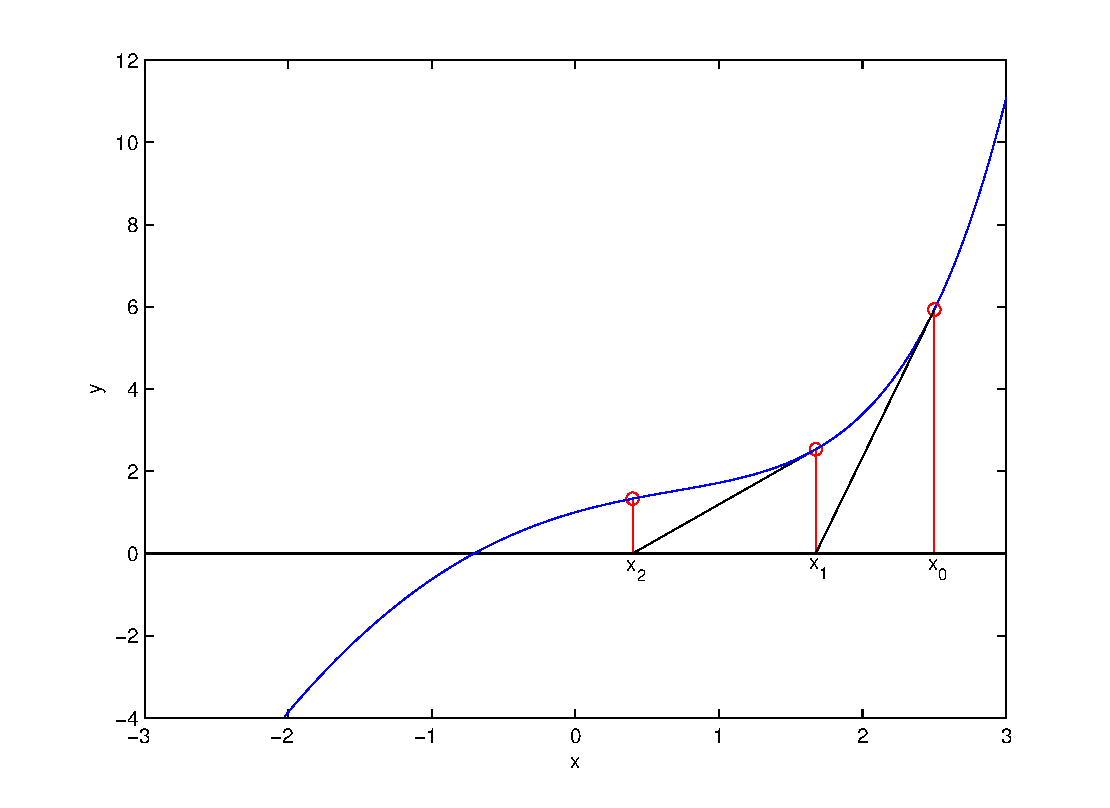
\includegraphics[width=7cm]{newt1.pdf}}\qquad
\subfigure[iteracion 3]{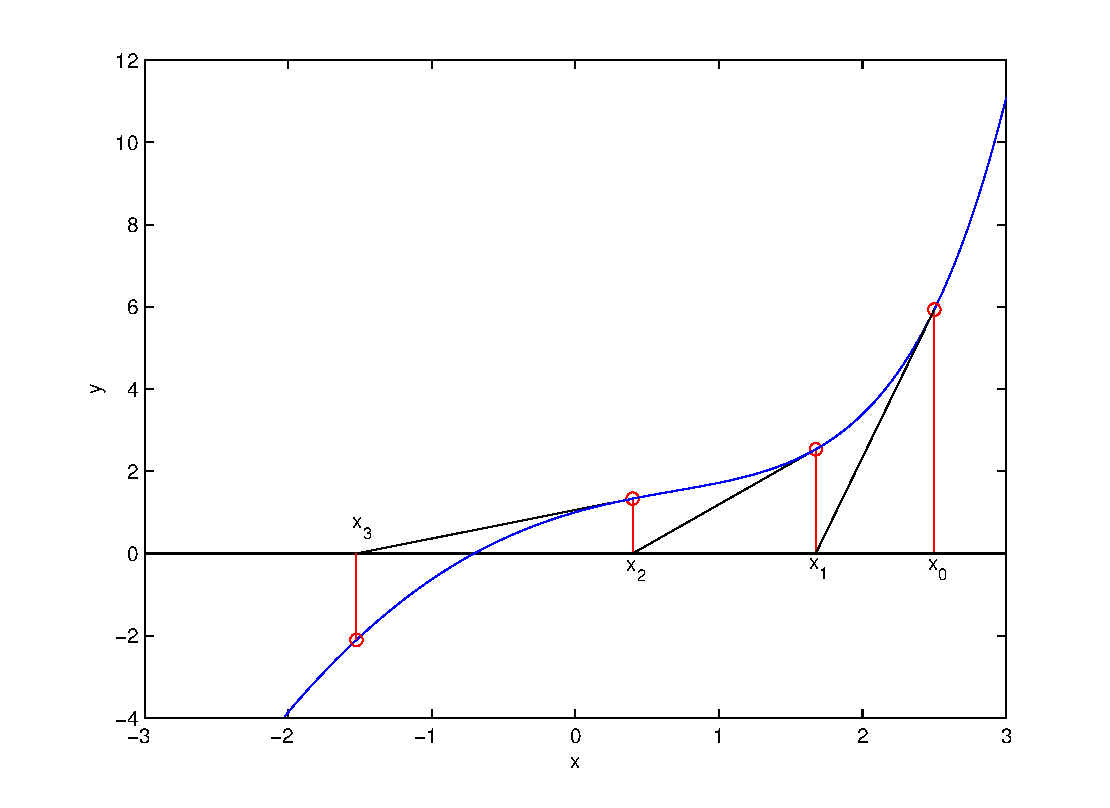
\includegraphics[width=7cm]{newt2.pdf}}\\
\subfigure[iteracion 4]{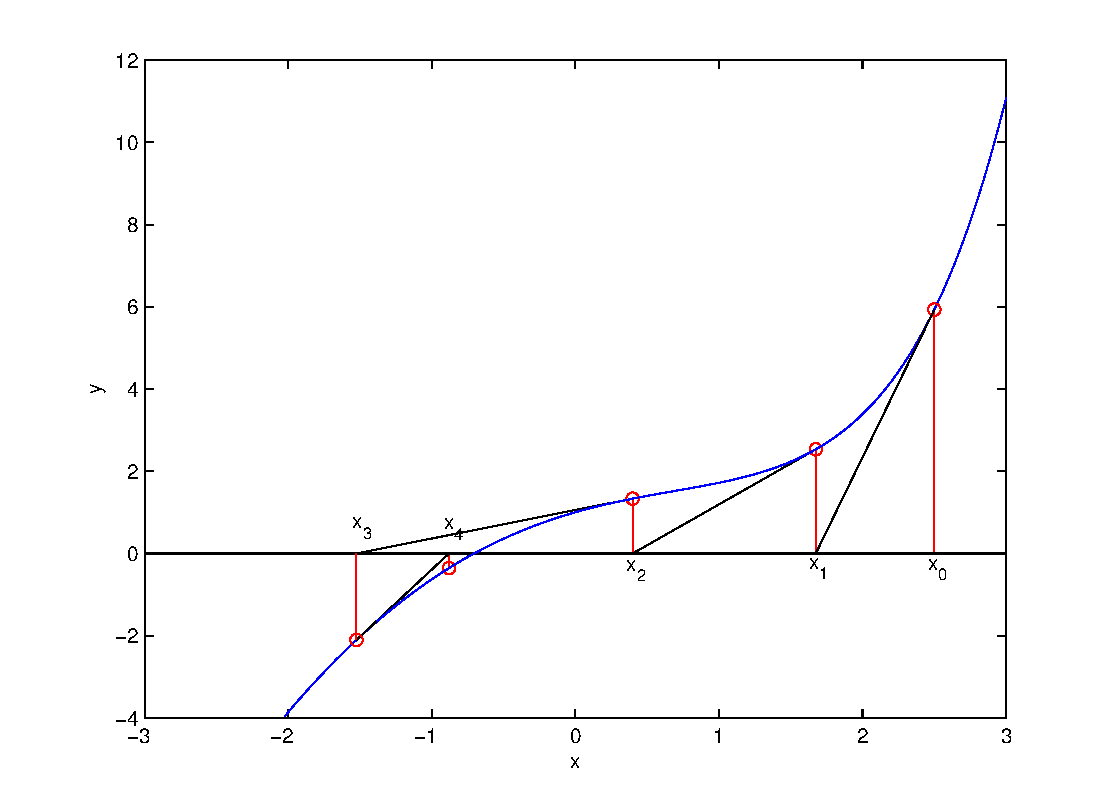
\includegraphics[width=7cm]{newt3.pdf}}\qquad
\subfigure[iteracion 5: raíz de la función]{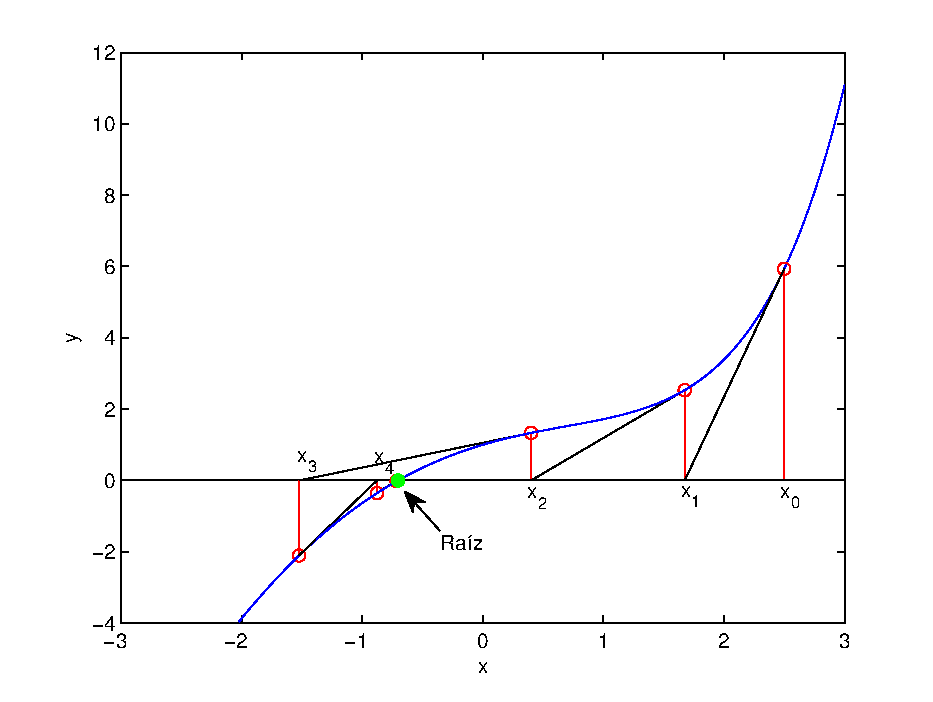
\includegraphics[width=7cm]{newt4.pdf}}

\bicaption{Proceso de obtención de la raíz de una función por el método de Newton}{Process of obtaining the root of a function by Newton's method}
\label{fig:newton2}
\end{figure}





\begin{paracol}{2}
La figura \ref{fig:newton2} muestra un ejemplo de obtención de la raíz de una función mediante el método de Newton. El método es más rápido que los dos anteriores, es decir, partiendo de una distancia comparable a la raíz, es el que converge en menos iteraciones. 

\switchcolumn

Figure \ref{fig:newton2} shows an example of obtaining the root of a function using Newton's method. The method is faster than the previous two, i.e., starting from a comparable distance to the root, it is the one that converges in the fewest iterations.

\switchcolumn

En el ejemplo de la figura se ha obtenido la raíz para la misma función que en los ejemplos del método de la bisección e interpolación lineal. Se ha empezado sin embargo en un punto más alejado de la raíz, para que pueda observarse mejor en la figura la evolución del algoritmo. En cada uno de los gráficos que componen la figura pueden observarse  los pasos del algoritmo: dado el punto  $x_i$, se calcula  la recta tangente a la función $f(x)$ en el punto y se obtiene un nuevo punto $x_{i+1}$,  como el corte de dicha recta tangente con el eje de abscisas.

\switchcolumn


In the example in the figure, the root has been obtained for the same function as in the examples of the bisection and false position method. However, we have started at a point further away from the root, so that the evolution of the algorithm can be better observed in the figure. In each of the graphs that make up the figure, the steps of the algorithm can be observed: given the point $x_i$, the tangent line to the function $f(x)$ at the point is calculated and a new point $x_{i+1}$ is obtained, as the intersection of this tangent line with the abscissa axis.

\switchcolumn

En este ejemplo el algoritmo converge en las cinco iteraciones que se muestran en la figura, para la misma tolerancia empleada en los métodos anteriores, $tol=0.01$. El punto de inicio empleado fue $x_0=2.5$, por tanto esta fuera del intervalo $[-2, 2]$ y más alejado de la raíz que en el caso de los métodos anteriores.   

\switchcolumn

In this example the algorithm converges in the five iterations shown in the figure, for the same tolerance used in the previous methods, $tol=0.01$. The starting point used was $x_0=2.5$, so it is outside the interval $[-2, 2]$ and further away from the root than in the case of the previous methods.   

\switchcolumn

\subsection{Método de la secante}
El método de la secante podría considerarse una variante del método de newton en el que se sustituye la recta tangente al punto $x0$ por la recta secante que une dos puntos obtenidos en iteraciones sucesivas. La idea es \emph{aproximar} la derivada a la función $f$ en el punto $x_n$ por la pendiente de una recta secante, es decir de una recta que corta a la función en dos puntos, 
\begin{equation*}
f'(x_n)\approx \frac{f(x_n)-f(x_{n-1})}{x_n-x_{n-1}}
\end{equation*}

\switchcolumn

\subsection{Secant method}
The secant method could be considered a variant of Newton's method in which the tangent line to the point $x0$ is replaced by the secant line joining two points obtained in successive iterations. The idea is to approximate the derivative of the function $f$ at the point $x_n$ by the slope of a secant line, i.e. a line that cuts the function at two points, 
\begin{equation*}
f'(x_n)\approx \frac{f(x_n)-f(x_{n-1})}{x_n-x_{n-1}}
\end{equation*}

\switchcolumn
Las sucesivas aproximaciones a la raíz de la función se obtienen de modo similar a las del método de Newton, simplemente sustituyendo la derivada de la función por su valor aproximado,

\begin{equation*}
x_{n+1}=x_n-\frac{f(x_n)}{f'(x_n)}\approx x_n-\frac{(x_n-x_{n-1})\cdot f(x_n)}{f(x_n)-f(x_{n-1})}
\end{equation*}

\switchcolumn
The successive approximations to the root of the function are obtained in a similar way to Newton's method, by simply substituting the derivative of the function by its approximate value,
\begin{equation*}
x_{n+1}=x_n-\frac{f(x_n)}{f'(x_n)}\approx x_n-\frac{(x_n-x_{n-1})\cdot f(x_n)}{f(x_n)-f(x_{n-1})}
\end{equation*}

\end{paracol}

\begin{figure}[h]
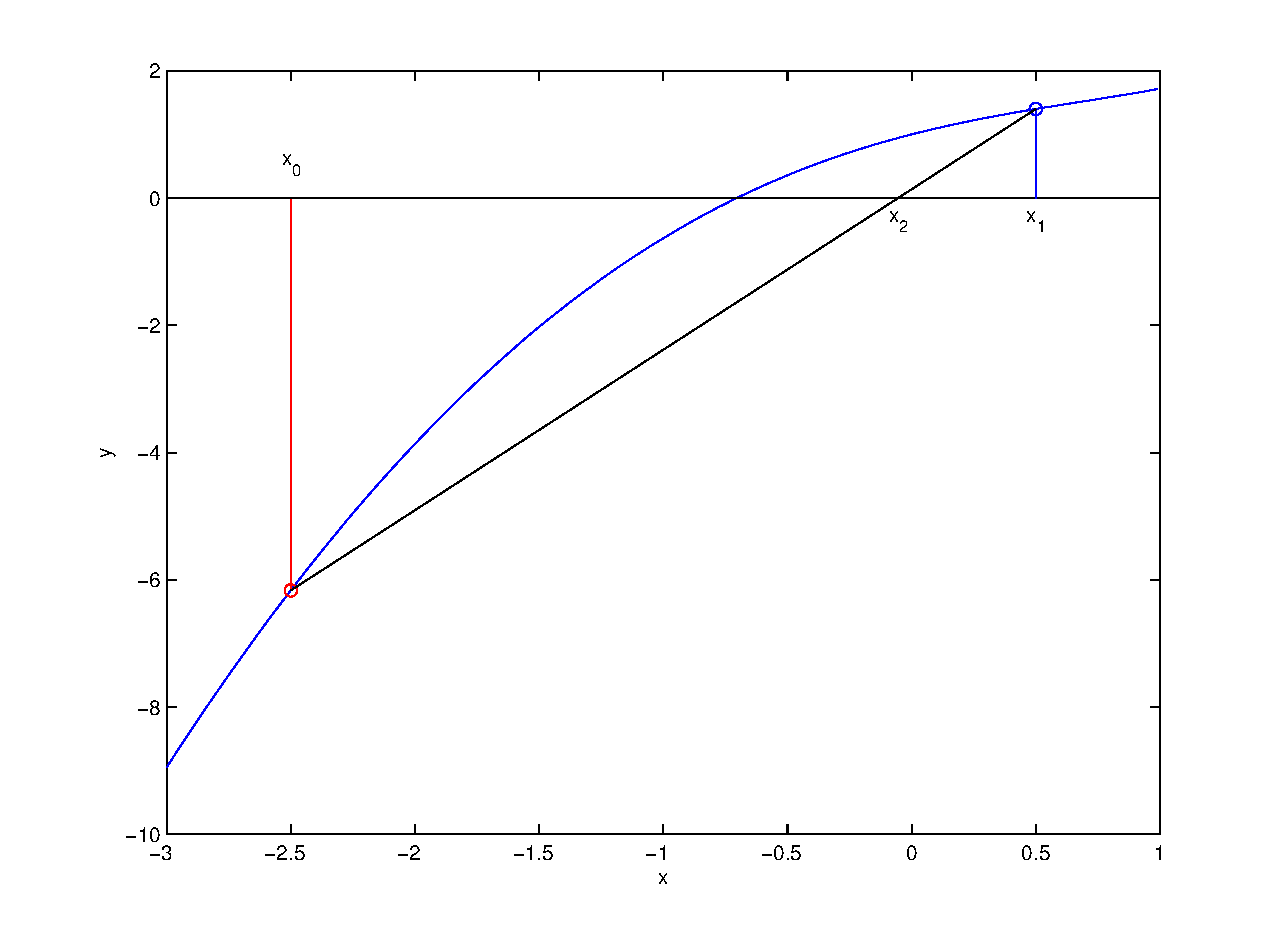
\includegraphics[width=14cm]{secante0.pdf}
\bicaption{Recta secante a la  función $f(x)$ en los puntos $x_0$ y $x_1$}{Secant line to the function $f(x)$ at points $x_0$ and $x_1$.}
\label{fig:secante}
\end{figure}

\begin{paracol}{2}
Para iniciar el algoritmo, es preciso emplear en este caso dos puntos iniciales. La figura \ref{fig:secante} muestra un ejemplo.

    \switchcolumn
    To start the algorithm, two starting points must be used in this case. Figure \ref{fig:secante} shows an example.
\switchcolumn
El método podría en este punto confundirse con el de interpolación, sin embargo tiene dos diferencias importantes: En primer lugar, la elección de los dos puntos iniciales $x_0$ e $x_1$, no tienen por qué formar un intervalo que contenga a la raíz. Es decir, podrían estar ambos situados al mismo lado de la raíz. En segundo lugar, los puntos obtenidos se van sustituyendo por orden, de manera que la nueva recta secante se construye siempre a partir de los dos últimos puntos obtenidos, sin prestar atención a que el valor de la raíz esté contenido entre ellos. (No se comparan los signos de la función en los puntos para ver cual se sustituye, como en el caso del método de interpolación). 

\switchcolumn
The method could at this point be confused with false position method, but it has two important differences: Firstly, the choice of the two initial points $x_0$ and $x_1$, need not form an interval containing the root. That is, they could both be located on the same side of the root. Secondly, the points obtained are substituted in order, so that the new secant line is always constructed from the last two points obtained, without paying attention to whether the value of the root is contained between them. (The signs of the function at the points are not compared to see which one is substituted, as in the case of the interpolation method). 

\end{paracol}

\begin{figure}[h]
\centering
\begin{tikzpicture}
%\usetikzlibrary{shapes.geometric}
\path (5,0) node(a) [rectangle,draw=blue, very thick,align=center,rounded corners]{Partimos de dos puntos inicial $x_0$, $x_1$}
(5,-2) node(b)[rectangle,draw=blue, thick,rounded corners,align=center]{Calculamos\\ $x=x_1-\frac{(x_1-x_0)\cdot f(x_1)}{f(x_1)-f(x_0)}, f(x)$}
(5,-4) node(c)[diamond,aspect=3,draw=red,thick]{es $\vert f(x) \vert \le \text{tol}$?}
(9,-4) node(d)[rectangle,draw=blue,align=center,very thick, rounded corners]{convergencia:\\ terminar}
(5,-6) node(g)[rectangle,draw=blue,thick,rounded corners,align=center]{$x_0=x_1$\\ $x_1=x$};
\draw[blue,-latex](a.south)--(b);
\draw[blue,-latex](b.south)--(c);
\draw[blue,-latex](c.east)--(d);
\draw (7.5,-4)node[above]{Sí};
\draw[blue,-latex](c.south)--(g);
\draw (5,-5)node[right]{No};
\draw[blue,-latex](g.south)|-(2,-7)|-(b);

\end{tikzpicture}
\caption{Diagrama de flujo del método de la secante}
\label{fig:secante2}
\end{figure}

\begin{figure}[h]
\centering
\begin{tikzpicture}
%\usetikzlibrary{shapes.geometric}
\path (5,0) node(a) [rectangle,draw=blue, very thick,align=center,rounded corners]{Begin with two initial points $x_0$, $x_1$}
(5,-2) node(b)[rectangle,draw=blue, thick,rounded corners,align=center]{Compute\\ $x=x_1-\frac{(x_1-x_0)\cdot f(x_1)}{f(x_1)-f(x_0)}, f(x)$}
(5,-4) node(c)[diamond,aspect=3,draw=red,thick]{is $\vert f(x) \vert \le \text{tol}$?}
(9,-4) node(d)[rectangle,draw=blue,align=center,very thick, rounded corners]{it converges:\\ finish}
(5,-6) node(g)[rectangle,draw=blue,thick,rounded corners,align=center]{$x_0=x_1$\\ $x_1=x$};
\draw[blue,-latex](a.south)--(b);
\draw[blue,-latex](b.south)--(c);
\draw[blue,-latex](c.east)--(d);
\draw (7.5,-4)node[above]{Yes};
\draw[blue,-latex](c.south)--(g);
\draw (5,-5)node[right]{No};
\draw[blue,-latex](g.south)|-(2,-7)|-(b);

\end{tikzpicture}
\caption{Flowchart of the secant method}
\label{fig:secante2_eng}
\end{figure}

\begin{paracol}{2}

La figura \ref{fig:secante2} muestra un diagrama de flujo para el método de la secante. El diagrama es básicamente el mismo que el empleado para el método de Newton. Las dos diferencias fundamentales son, que ahora en lugar de evaluar la función y la derivada en cada iteración, se calcula  el valor del punto de corte de la recta que pasa por los dos últimos puntos obtenidos (es decir, empleamos una recta secante, que corta a la curva en dos puntos, en lugar de emplear una recta tangente). 

\switchcolumn
Figure \ref{fig:secante2_eng} shows a flow diagram for the secant method. The diagram is basically the same as the one used for Newton's method. The two fundamental differences are that now, instead of evaluating the function and the derivative at each iteration, we calculate the value of the cut-off point of the line passing through the last two points obtained (i.e. we use a secant line, which cuts the curve at two points, instead of using a tangent line). 

\switchcolumn

Además es preciso actualizar, en cada iteración, el valor de los dos últimos puntos obtenidos: el más antiguo se desecha, el punto recién obtenido sustituye al anterior y éste al obtenido dos iteraciones antes. 

\switchcolumn

In addition, the value of the last two points obtained must be updated in each iteration: the oldest point is discarded, the newly obtained point replaces the previous one and this one replaces the one obtained two iterations before. 


\end{paracol}

\begin{figure}
\centering
\subfigure[intervalo inicial]{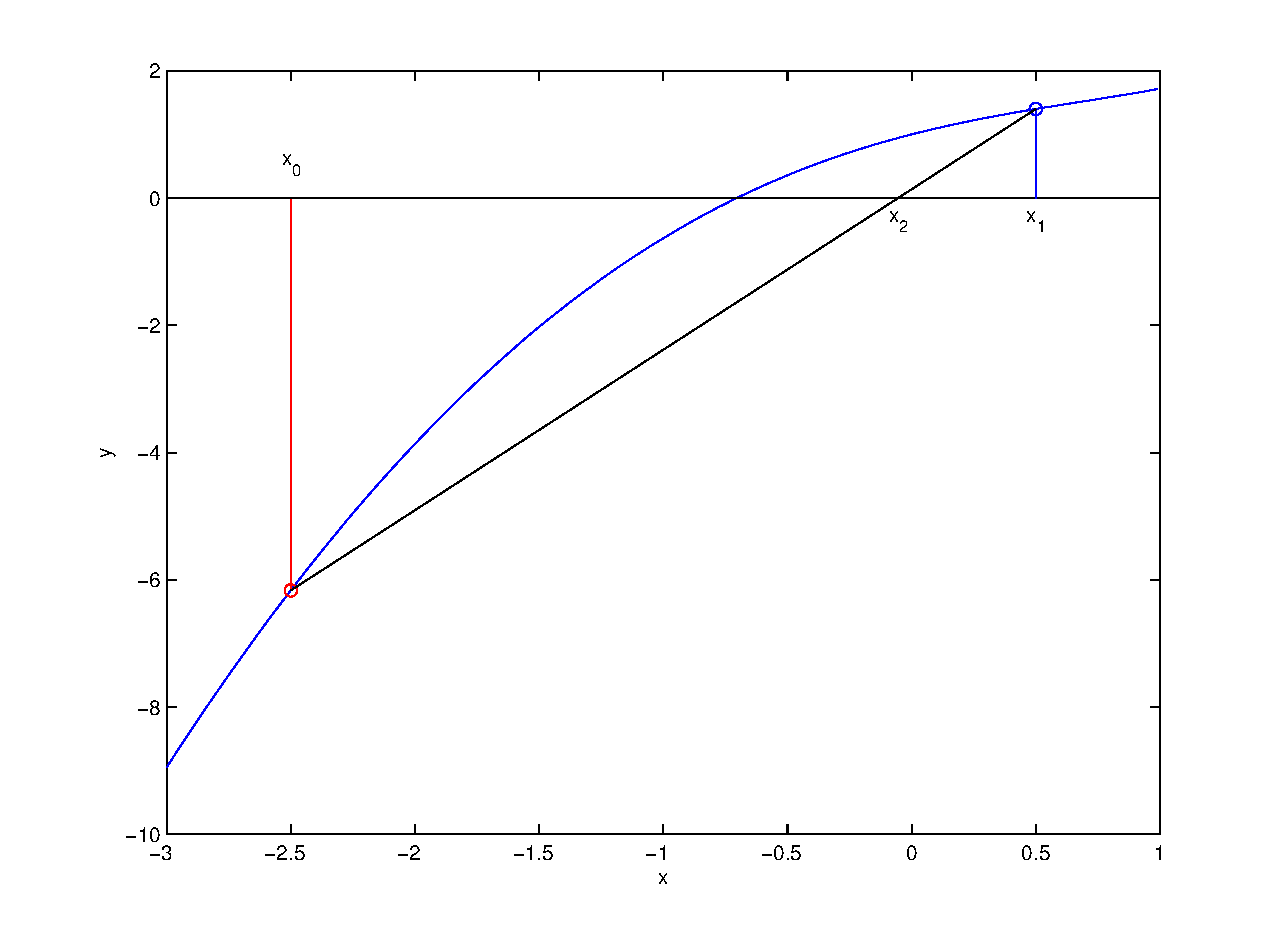
\includegraphics[width=7cm]{secante0.pdf}} \qquad
\subfigure[iteracion 1]{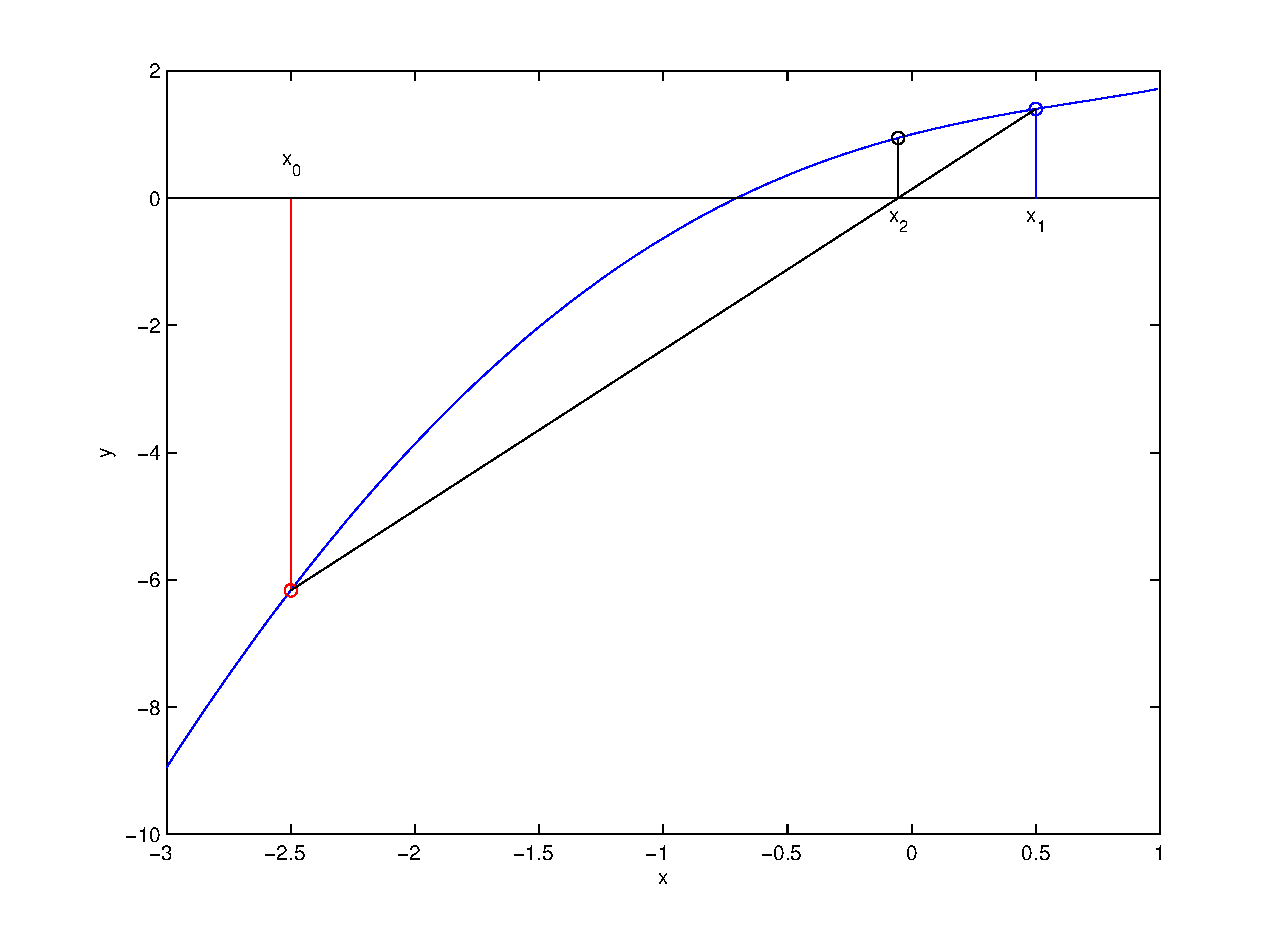
\includegraphics[width=7cm]{secante1.pdf}}\\
\subfigure[iteración 2]{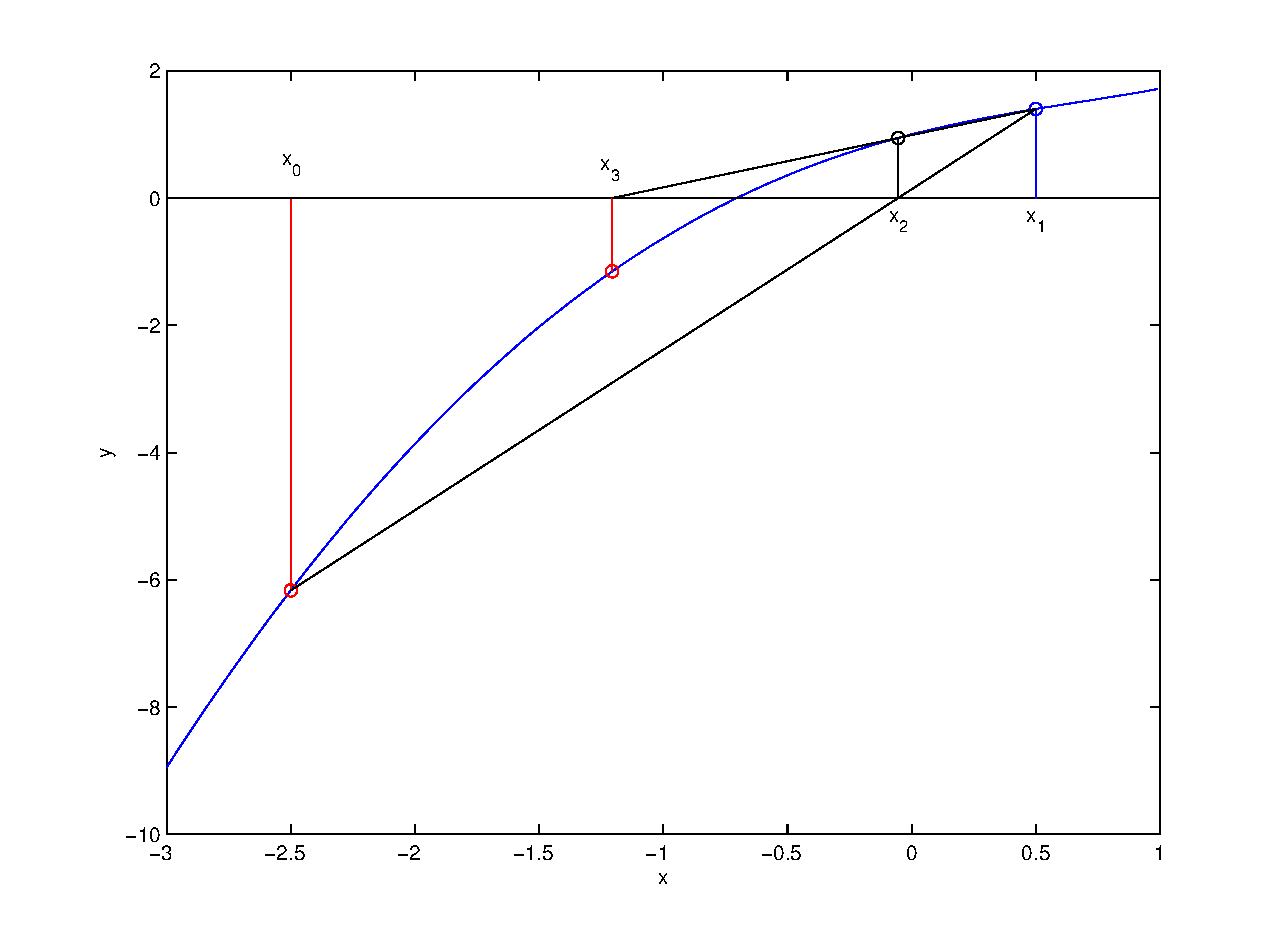
\includegraphics[width=7cm]{secante2.pdf}}\qquad
\subfigure[iteración 3]{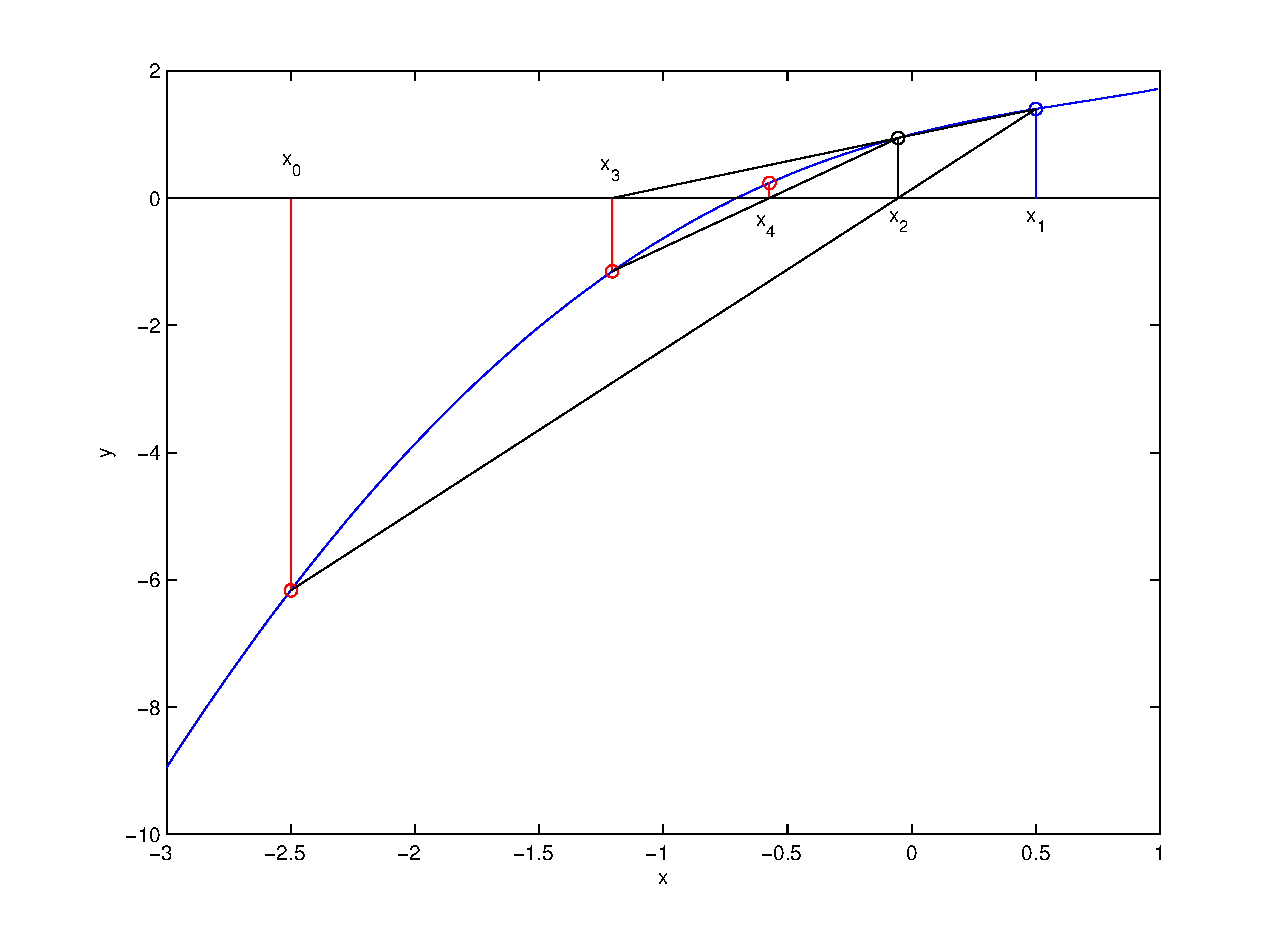
\includegraphics[width=7cm]{secante3.pdf}}\\
\subfigure[iteración 4]{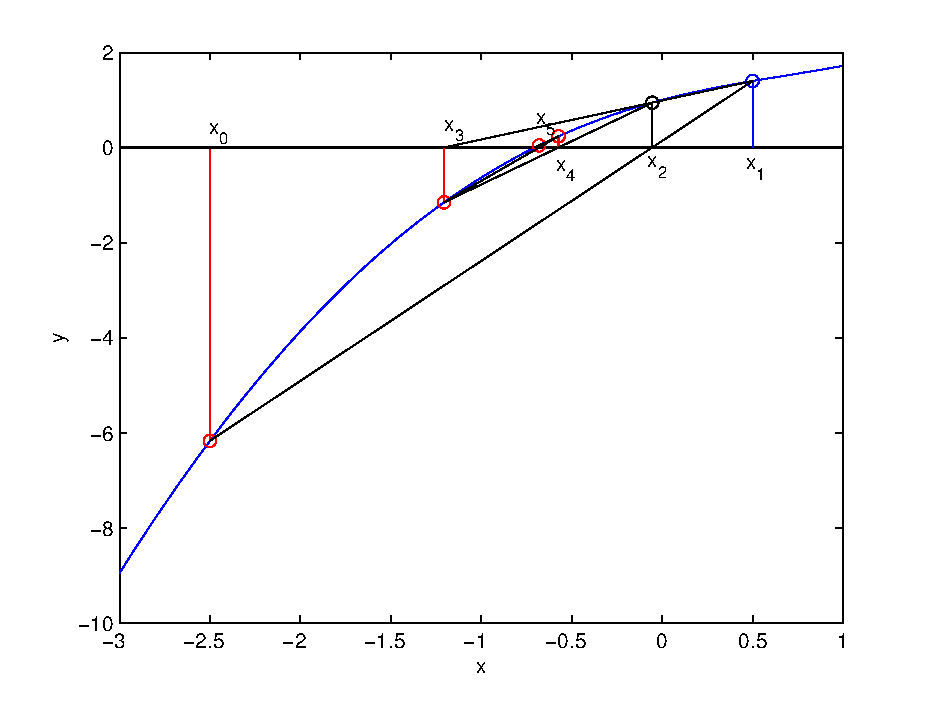
\includegraphics[width=7cm]{secante31.pdf}}\qquad
\subfigure[iteración 5]{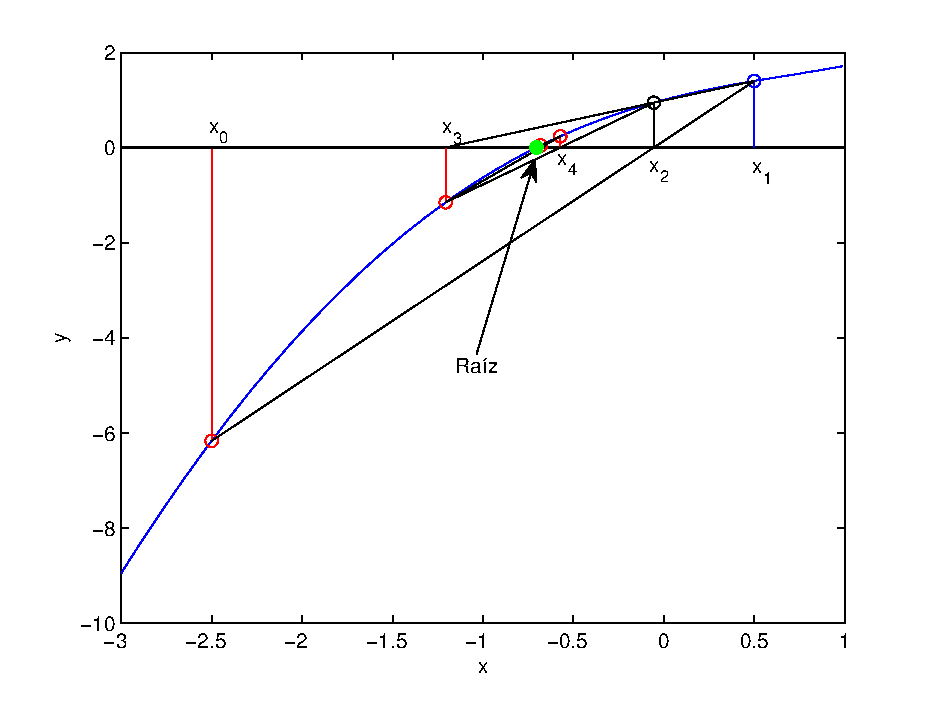
\includegraphics[width=7cm]{secante4.pdf}}

\caption{proceso de obtención de la raíz de una función por el método de la secante}{process of obtaining the root of a function by the secant method}
\label{fig:secante3}
\end{figure}

\begin{paracol}{2}
La figura \ref{fig:secante3} muestra un ejemplo de la obtención de una raíz por el método de la secante. Se ha empleado de nuevo la misma función que en los ejemplos anteriores, tomando como valores iniciales, $x_0=-2.5$ y $x_1=0.5$. La tolerancia se ha fijado en $tol=0.01$ también como en los anteriores algoritmos descritos. En este caso, el algoritmo encuentra la raíz en cinco iteraciones. Cada uno de los gráficos que compone la figura \ref{fig:secante3}, muestra la obtención de un nuevo punto a partir de los dos anteriores. 

    \switchcolumn
Figure \ref{fig:secante3} shows an example of obtaining a root by the secant method. The same function has been used again as in the previous examples, taking as initial values, $x_0=-2.5$ and $x_1=0.5$. As in the previous algorithms described, the tolerance has been set to $tol=0.01$. In this case, the algorithm finds the root in five iterations. Each of the graphs that make up the figure \ref{fig:secante3}, shows the obtaining of a new point from the previous two. 
    \switchcolumn

En la iteración 2, puede observarse como el nuevo punto se obtiene a partir de dos puntos que están ambos situados a la derecha de la raíz, es decir, no forman un intervalo que contenga a la raíz.  Aquí se pone claramente de manifiesto la diferencia con el método de interpolación lineal. De hecho, com ya se ha dicho, el método de la secante puede iniciarse tomando los dos primeros puntos a uno de los lados de la raíz.

\switchcolumn
In iteration 2, it can be seen how the new point is obtained from two points that are both located to the right of the root, i.e. they do not form an interval containing the root.  Here the difference with the linear interpolation method is clearly shown. In fact, as already mentioned, the secant method can be started by taking the first two points on either side of the root.

\switchcolumn
 El método es, en principio, más eficiente que el de la bisección y el de interpolación lineal, y menos eficiente que el de Newton.
\switchcolumn

 The method is, in principle, more efficient than bisection and false position, and less efficient than Newton's method.

 \switchcolumn
 La ventaja de este método respecto al de Newton es que evita tener que calcular explícitamente la derivada de la función para la que se quiere calcular la raíz. El algunos casos, la obtención de la forma analítica de dicha derivada puede ser compleja.   
\switchcolumn

The advantage of this method over Newton's is that it avoids having to explicitly calculate the derivative of the function for which the root is to be calculated. In some cases, obtaining the analytical form of this derivative can be complex.  

\end{paracol}

\begin{paracol}{2}




 \subsection{Método de las aproximaciones sucesivas o del punto fijo}\label{pfijo}

El método del punto fijo es, como se verá a lo largo de esta sección, el más sencillo de programar de todos. Desafortunadamente, presenta el problema de que no podemos aplicarlo a todas las funciones. Hay casos en los que el método no converge, con lo que no es posible emplearlo para encontrar la raíz o raíces de una función.
 \switchcolumn


\subsection{Method of successive approximations or fixed point iteration}\label{pfijo}

The fixed point iteration is, as will be seen throughout this section, the simplest of all to program. Unfortunately, it has the problem that we cannot apply it to all functions. There are cases in which the method does not converge, so it is not possible to use it to find the root or roots of a function.

\switchcolumn

\paragraph{Punto fijo de una función.} \index{Punto fijo! de una función}Se dice que un punto $x_f$ es un punto fijo de una función $g(x)$ si se cumple,
\begin{equation*}
g(x_f)=x_f
\end{equation*}

Es decir, la imagen del punto fijo $x_f$ es de nuevo el punto fijo. Así por ejemplo la función,
\begin{equation*}
g(x)=-\sqrt{e^x}
\end{equation*}

Tiene un punto fijo en $x_f=-0.703467$, porque $g(-0.703467)=-0.703467$. La existencia de un punto fijo puede obtenerse gráficamente, representando en un mismo gráfico la función $y=g(x)$ y la recta $y=x$. Si existe un punto de corte entre ambas gráficas, se trata de un punto fijo.  La figura \ref{fig:pfijo0}, muestra gráficamente el punto fijo de la función $g(x)=-\sqrt{e^x}$ del ejemplo anterior.

Una función puede tener uno o más puntos fijos o no tener ninguno. Por ejemplo, la función $y=\sqrt{e^x}$ no tiene ningún punto fijo.

\switchcolumn
\paragraph{Fixed point.} \index{Fixed point!} $x_f$ is a fixed point of $g(x)$ if it holds,
\begin{equation*}
g(x_f)=x_f
\end{equation*}

That is, the image of the fixed point $x_f$ is again the fixed point. So for example the function,
\begin{equation*}
g(x)=-\sqrt{e^x}
\end{equation*}

Has a fixed point  $x_f=-0.703467$, because $g(-0.703467)=-0.703467$. The existence of a fixed point can be obtained graphically, representing in the same graph the function $y=g(x)$ and the straight line $y=x$. If there is a point of intersection between both graphs, it is a fixed point. The figure \ref{fig:pfijo0}, shows graphically the fixed point of the function $g(x)=-\sqrt{e^x}$ of the previous example.

A function can have one or more fixed points or none at all. For example, the function $y=\sqrt{e^x}$ does not have any fixed point.
\end{paracol}

\begin{figure}[h]
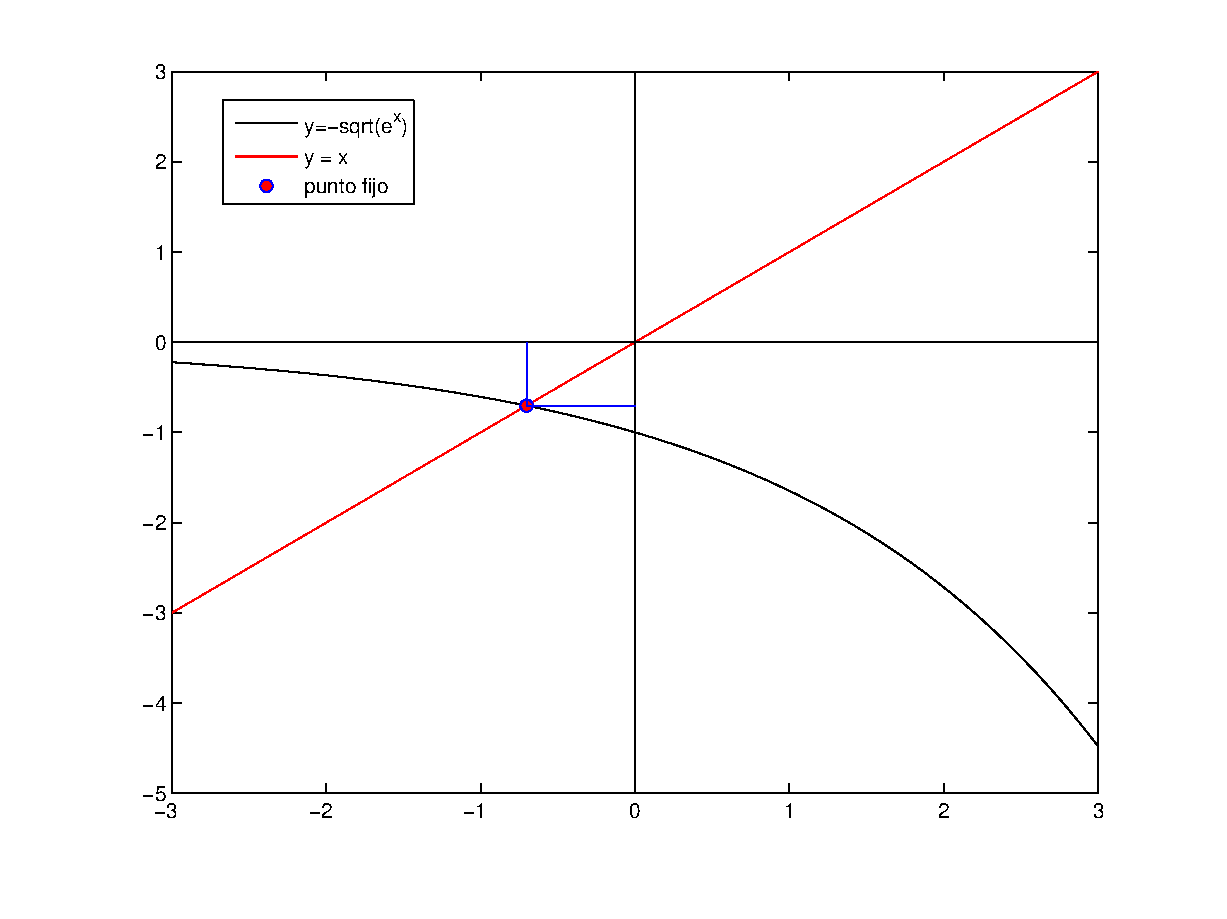
\includegraphics[width=14cm]{pfijo0.eps}
\bicaption{Obtención gráfica del punto fijo de la función, $g(x)=-\sqrt{e^x}$}{Obtaining the fixed point of the function graphically, $g(x)=-\sqrt{e^x}$}
\label{fig:pfijo0}
\end{figure}


\begin{paracol}{2}

\paragraph{Punto fijo atractivo.} \index{Punto fijo! atractivo}Supongamos ahora que, a partir de la función $g(x)$ creamos la siguiente sucesión,
\begin{equation*}
x_{n+1}=g(x_n)
\end{equation*}

Es decir, empezamos tomando un punto inicial $x_0$ y a partir de él vamos obteniendo los siguientes valores de la sucesión como,
\switchcolumn

\paragraph{Attracting fixed point.} \index{Attracting fixed point} SSuppose now that from the function $g(x)$ we create the following sequence,
\begin{equation*}
x_{n+1}=g(x_n)
\end{equation*}

That is, we start by taking an initial point $x_0$and from it we obtain the following values of the sequence as,
\end{paracol}
\begin{equation*}
x_0\rightarrow x_1=g(x_0)\rightarrow x_2=g(x_1)=g\left(g(x_0)\right) \rightarrow \cdots \rightarrow x_{n+1}=g(x_{n})=g\left( g\left( \cdots\left( g(x_0)\right)\right)\right) \rightarrow \cdots
\end{equation*}

\begin{paracol}{2}
Decimos que un punto fijo $x_f$ de la función $g(x)$ es un punto fijo atractivo si la sucesión $x_{n+1}=g(x_n)$ converge al valor $x_f$, siempre que $x_0$ se tome \emph{suficientemente} cercano a $x_f$. Cómo de cerca tienen que estar $x_0$ y $x_f$ para que la serie converja, es una cuestión delicada. De entrada, es importante descartar que hay funciones que tienen puntos fijos no atractivos, por ejemplo, la función $g(x)=x^2$ tiene dos puntos fijos $x=0$ y $x=1$. El primero es el límite de la sucesión $x_{n+1}=g(x_n)$ para cualquier valor inicial $x_0$ contenido en el intervalo abierto $(-1,  1)$. El punto $x=1$ resulta inalcanzable para cualquier sucesión excepto que el punto de inicio sea él mismo $x_0=x_f=1$.

Hay algunos casos en los que  es posible, para determinadas funciones, saber cuando uno de sus puntos fijos es atractivo,
\switchcolumn

We can say that fixed point $x_f$ of function $g(x)$ is an attracting  fixed point if the succession $x_{n+1}=g(x_n)$ converges to $x_f$, if $x_0$ is close \emph{enough} to $x_f$. How close $x_0$ and $x_f$ have to be for the series to converge is a delicate question. For example, the function $g(x)=x^2$ has two fixed points $x=0$ and $x=1$. The first is the limit of the sequence $x_{n+1}=g(x_n)$ for any initial value $x_0$ contained in the open interval $(-1, 1)$. The point $x=1$ is unreachable for any sequence unless the starting point is itself $x_0=x_f=1$.

There are some cases where it is possible, for certain functions, to know when one of your fixed points is attractive,

\switchcolumn

\paragraph{Teorema de existencia y unicidad del punto fijo.}\index{Punto fijo! Teorema} Dada una función $g(x)$,  continua y diferen-\- ciable en un intervalo $[a, b]$, si se cumple que, $\forall x \in [a, b] \Rightarrow g(x)\in [a,b]$,  entonces $g(x)$ tiene un punto fijo en el intervalo $[a, b]$. 

Si además existe una constante positiva $k < 1$  y se  cumple que  la derivada $\vert g'(x) \vert \leq k, \  \forall x \in (a, b)$, entonces el punto fijo contenido en $[a,b]$ es único. 

Para demostrar la primera parte del teorema, se puede emplear el teorema de Bolzano. Si se cumple que $g(a)=a$ o que  $g(b)=b$, entonces $a$ o $b$ serían el punto fijo. Supongamos que no es así;  entonces tiene que cumplirse que $g(a)>a$ y que $g(b)<b$. Si construimos una función, $f(x)=g(x)-x$ esta función, que es continua por construcción, cumple que $f(a)=g(a)-a>0$ y $f(b)=g(b)-b<0$. Pero entonces, debe existir un punto, $x_f \in [a, b]$ para el cual $f(x_f)=0$ y, por tanto, $f(x_f)=g(x_f)-x_f=0 \Rightarrow g(x_f)=x_f$. Es decir, $x_f$ es un punto fijo de $g(x)$.

La segunda parte del teorema puede demostrarse empleando el teorema de valor medio. Si suponemos  que existen dos puntos fijos distintos $x_{f1} \neq x_{f2}$ en el intervalo $[a,b]$, según el teorema del valor medio, existe un punto $\xi$ comprendido entre $x_{f1}$ y $ x_{f2}$ para el que se cumple,

\begin{equation*}
\frac{g(x_{f1})-g(x_{f2})}{x_{f1}-x_{f2}}=g'(\xi)
\end{equation*}
\switchcolumn

\paragraph{Fixed point theorem.}\index{Fixed point! theorem} Let $g(x)$ , be a continuous and derivable function in $[a, b]$, if, $\forall x \in [a, b] \Rightarrow g(x)\in [a,b]$,  then $g(x)$ has at least a fixed point in $[a, b]$. 

If, in addition, there is a positive constant $k < 1$  and it holds that  $\vert g'(x) \vert \leq k, \  \forall x \in (a, b)$, then $g(x)$ has a unique fixed point in $[a,b]$. 

To prove the first part of the theorem, Bolzano's theorem can be used. If it is satisfied that $g(a)=a$ or $g(b)=b$, then $a$ or $b$ would be the fixed point. Suppose this is not the case; then it must be true that $g(a)>a$ and that $g(b)<b$. Define $f(x)=g(x)-x$. This function, which is continuous by construction, satisfies that $f(a)=g(a)-a>0$ and $f(b)=g(b)-b<0$. Then, there is a $x_f \in [a, b]$ that holds $f(x_f)=0$ and therefore $f(x_f)=g(x_f)-x_f=0 \Rightarrow g(x_f)=x_f$. That is, $x_f$ is a fixed point of $g(x)$.

The second part of the theorem can be proved using the mean value theorem. If we assume that there are two distinct fixed points $x_{f1} \neq x_{f2}$ in $[a,b]$, according to the mean value theorem, there exists a point $\xi$ between $x_{f1}$ and $x_{f2}$ for which it is satisfied,

\begin{equation*}
\frac{g(x_{f1})-g(x_{f2})}{x_{f1}-x_{f2}}=g'(\xi)
\end{equation*}

Therefore,
\end{paracol}


\begin{equation*}
\vert g(x_{f1})-g(x_{f2}) \vert =\vert x_{f1}-x_{f2} \vert\cdot \vert g'(\xi) \vert \leq \vert x_{f1}-x_{f2} \vert \cdot k < \vert x_{f1}-x_{f2} \vert 
\end{equation*}

\begin{paracol}{2}

Pero como se trata de puntos fijos $\vert g(x_{f1})-g(x_{f2}) \vert =\vert x_{f1}-x_{f2}\vert $. con lo que llegaríamos al resultado contradictorio, 

\switchcolumn

But since we are dealing with fixed points $\vert g(x_{f1})-g(x_{f2}) \vert =vert x_{f1}-x_{f2} \vert$, this would lead to the contradictory result

\end{paracol}

 \begin{equation*}
\vert x_{f1}-x_{f2}\vert=\vert g(x_{f1})-g(x_{f2}) \vert  \leq \vert x_{f1}-x_{f2} \vert\cdot k < \vert x_{f1}-x_{f2} \vert 
\end{equation*}

\begin{paracol}{2}
Salvo que, en contra de la hipótesis inicial, se cumpla que  $ x_{f1}=x_{f2}$. En cuyo caso, solo puede existir un único punto fijo en el intervalo $[a, b]$ bajo las condiciones impuestas por el teorema.

\switchcolumn
Unless, contrary to the initial hypothesis, it is satisfied that $ x_{f1}=x_{f2}$. In which case, there can only be a single fixed point in the interval $[a, b]$ under the conditions imposed by the theorem.

\switchcolumn

\paragraph{Teorema de punto fijo (atractivo).} \footnote{Hay varios teoremas de punto fijo definidos en distintos contextos matemáticos. Aquí se da una versión reducida a funciones $f(x):\mathbb{R} \rightarrow \mathbb{R}$} Dada una función $g(x)$,  continua y diferenciable en un intervalo $[a, b]$, que  cumple que, $\forall x \in [a, b] \Rightarrow g(x)\in [a,b]$ y que  $\vert g'(x) \vert \leq k, \  \forall x \in (a, b)$, con $0<k<1$, entonces se cumple que, para cualquier punto inicial $x_0$, contenido en el intervalo $[a, b]$, la sucesión  $x_{n+1}=g(x_n)$ converge al único punto fijo del intervalo $[a, b]$.
La demostración puede obtenerse de nuevo a partir del teorema del valor medio. Si lo aplicamos al valor inicial $x_0$ y al punto fijo $x_f$, obtenemos,
\switchcolumn

\paragraph{Theorem of the attracting fixed point.} \footnote{There are several fixed point theorems defined in different mathematical contexts. A version reduced to functions $f(x):\mathbb{R} \rightarrow \mathbb{R}$ is given here.} Let $g(x)$,  continuous and differentiable on an interval $[a, b]$, that holds, $\forall x \in [a, b] \Rightarrow g(x)\in [a,b]$ and that  $\vert g'(x) \vert \leq k, \  \forall x \in (a, b)$, with $0<k<1$, then it holds that for any $x_0$, in $[a, b]$, the succession  $x_{n+1}=g(x_n)$ converges to the only fixed point of the interval $[a, b]$.
The proof can again be obtained from the mean value theorem. If we apply it to the initial value $x_0$ and the fixed point $x_f$, we obtain,

\begin{equation*}
\vert g(x_0)-g(x_f) \vert =\vert x_0-x_f \vert \cdot \vert g'(\xi) \vert \leq \vert x_0-x_f \vert \cdot k 
\end{equation*}

\switchcolumn
Para la siguiente iteración tendremos,

\begin{equation*}
\vert g(x_1)-g(x_f) \vert \leq \vert x_1-x_f \vert \cdot k \leq \vert x_0-x_f \vert \cdot k^2 
\end{equation*}

puesto que,  $x_1=g(x_0)$ y $x_f = g(x_f)$, puesto que $x_f$ es el punto fijo. 

Por simple inducción tendremos que para el término enésimo de la sucesión,
\switchcolumn
For the next iteration we will have,

\begin{equation*}
\vert g(x_1)-g(x_f) \vert \leq \vert x_1-x_f \vert \cdot k \leq \vert x_0-x_f \vert \cdot k^2 
\end{equation*}

since $x_1=g(x_0)$ y $x_f = g(x_f)$, because $x_f$ is a fixed point.

Using induction we can obtain the ntn term of the sequence,
\end{paracol}
\begin{equation*}
\vert g(x_n)-g(x_f) \vert \leq \vert x_{n-1}-x_f \vert \cdot k \leq \vert x_{n-2}-x_f \vert \cdot k^2 \leq \cdots \leq  \vert x_0-x_f \vert \cdot k^n 
\end{equation*}

\begin{paracol}{2}
Pero

\switchcolumn
But,
\end{paracol}

\begin{equation*}
\underset{n\rightarrow \infty}{\text{lim}}k^n=0 \Rightarrow \underset{n\rightarrow \infty}{\text{lim}} \vert x_n-x_f \vert \leq \underset{n\rightarrow \infty}{\text{lim}}\vert x_0-x_f \vert k^n =0
\end{equation*} 

\begin{paracol}{2}
Es decir, la sucesión  $x_{n+1}=g(x_n)$ converge al punto fijo $x_f$.

\switchcolumn
That is, the sequence $x_{n+1}=g(x_n)$ converges to the fixed point $x_f$.
\switchcolumn
\paragraph{El método del punto fijo.}\index{Punto fijo! Método} Como ya hemos visto, obtener una raíz de una función $f(x)$, consiste en resolver la ecuación $f(x)=0$. Supongamos que podemos descomponer la función $f(x)$ como la diferencia de dos términos, una función auxiliar, $g(x)$, y la propia variable $x$
\begin{equation*}
f(x)=g(x)-x
\end{equation*}
\switchcolumn
\paragraph{Fixed point iteration.}\index{Fijex point! Iteration} As we have already seen, obtaining a root of a function $f(x)$, consists of solving the equation $f(x)=0$. Suppose we can decompose the function $f(x)$ as the difference of two terms, an auxiliary function, $g(x)$, and the variable $x$ itself.
\begin{equation*}
f(x)=g(x)-x
\end{equation*}

\switchcolumn

Encontrar una raíz de $f(x)$ resulta entonces equivalente a buscar un punto fijo de $g(x)$. 

\begin{equation*}
f(x)=0 \rightarrow g(x)-x=0 \rightarrow g(x)=x
\end{equation*}

\switchcolumn


Finding a root of $f(x)$ is then equivalent to finding a fixed point of $g(x)$.

\begin{equation*}
f(x)=0 \rightarrow g(x)-x=0 \rightarrow g(x)=x
\end{equation*}

\switchcolumn

En general, a partir de una función dada $f(x)$, es posible encontrar distintas funciones $g(x)$ que cumplan que $f(x)=g(x)-x$. No podemos garantizar que cualquiera de las descomposiciones que hagamos nos genere una función $g(x)$ que tenga un punto fijo. 
Además, para funciones que tengan más de una raíz, puede suceder que distintas descomposiciones de la función converjan a distintas raíces.
Si podemos encontrar una que cumpla las condiciones del teorema de punto fijo que acabamos de enunciar, en un entorno de una raíz de $f(x)$, podemos desarrollar un método que obtenga iterativamente los valores de la sucesión   $x_{n+1}=g(x_n)$, a partir de un valor inicial $x_0$.  El resultado se aproximará al punto fijo de $g(x)$, y por tanto a la raíz de $f(x)$ tanto como queramos. Bastará, como   en los métodos anteriores, definir un valor (tolerancia), por debajo del cual consideramos que el valor obtenido es suficientemente próximo a  la raíz como para darlo por válido. 

La figura \ref{fig:pfijo1} muestra un diagrama de flujo del método del punto fijo. 

\switchcolumn

In general, starting from a given function $f(x)$, it is possible to find different functions $g(x)$ that satisfy that $f(x)=g(x)-x$. We cannot guarantee that any of the decompositions we do will generate a function $g(x)$ that has a fixed point. 
Moreover, for functions that have more than one root, it can happen that different decompositions of the function converge to different roots.
If we can find one that satisfies the conditions of the fixed point theorem just stated, in an environment of a root of $f(x)$, we can develop a method that iteratively obtains the values of the sequence $x_{n+1}=g(x_n)$, starting from an initial value $x_0$. The result will approximate the fixed point of $g(x)$, and therefore the root of $f(x)$ as much as we want. It will suffice, as in the previous methods, to define a value (tolerance), below which we consider that the value obtained is sufficiently close to the root to be valid.

Figure \ref{fig:fixedp} shows a flowchart of the fixed point iteration. 


\switchcolumn

\begin{figure}[h]
\centering
\begin{tikzpicture}
%\usetikzlibrary{shapes.geometric}
\path (5,0) node(a) [rectangle,draw=blue, very thick,align=center,rounded corners]{Partimos de un punto inicial $x_0$}
(5,-2) node(b)[rectangle,draw=blue, thick,rounded corners,align=center]{Calculamos\\ $x=g(x_0)$}
(5,-4) node(c)[diamond,aspect=3,draw=red,thick]{es $\vert  x-x_0 \vert \le \text{tol}$?}
(9,-4) node(d)[rectangle,draw=blue,align=center,very thick, rounded corners]{convergencia:\\ terminar}
(5,-6) node(g)[rectangle,draw=blue,thick,rounded corners,align=center]{$x_0=x$};
\draw[blue,-latex](a.south)--(b);
\draw[blue,-latex](b.south)--(c);
\draw[blue,-latex](c.east)--(d);
\draw (7.5,-4)node[above]{Sí};
\draw[blue,-latex](c.south)--(g);
\draw (5,-5)node[right]{No};
\draw[blue,-latex](g.south)|-(2,-7)|-(b);

\end{tikzpicture}
\caption{Diagrama de flujo del método del punto fijo. Nótese que la raíz obtenida corresponde a la función $f(x)=g(x)-x$}
\label{fig:pfijo1}
\end{figure}

\switchcolumn


\begin{figure}[h]
\centering
\begin{tikzpicture}
%\usetikzlibrary{shapes.geometric}
\path (5,0) node(a) [rectangle,draw=blue, very thick,align=center,rounded corners]{Initial point $x_0$}
(5,-2) node(b)[rectangle,draw=blue, thick,rounded corners,align=center]{Compute\\ $x=g(x_0)$}
(5,-4) node(c)[diamond,aspect=3,draw=red,thick]{is $\vert  x-x_0 \vert \le \text{tol}$?}
(9,-4) node(d)[rectangle,draw=blue,align=center,very thick, rounded corners]{it converges:\\ The end}
(5,-6) node(g)[rectangle,draw=blue,thick,rounded corners,align=center]{$x_0=x$};
\draw[blue,-latex](a.south)--(b);
\draw[blue,-latex](b.south)--(c);
\draw[blue,-latex](c.east)--(d);
\draw (7.5,-4)node[above]{Yes};
\draw[blue,-latex](c.south)--(g);
\draw (5,-5)node[right]{No};
\draw[blue,-latex](g.south)|-(2,-7)|-(b);

\end{tikzpicture}
\caption{Flowchart of fixed point iteration. Root corresponds to $f(x)=g(x)-x$}
\label{fig:fixedp}
\end{figure}


\switchcolumn

 La idea es elegir cuidadosamente el punto inicial $x_0$, para asegurar que se encuentra dentro del intervalo de convergencia del punto fijo.  A continuación, calculamos el valor de $g(x_0)$, el resultado será un nuevo valor  $x$ .  Comprobamos la diferencia entre el punto obtenido y el anterior y si es menor que una cierta tolerancia,  consideramos que el método ha convergido, dejamos de iterar, y devolvemos el valor de $x$ obtenido como resultado. Si no, copiamos $x$ en $x_0$ y volvemos a empezar todo el proceso. Es interesante hacer notar que que el algoritmo converge cuando la diferencia entre dos puntos consecutivos es menor que un cierto valor.  De acuerdo con la \emph{condición } de punto fijo $g(x_0)=x_0$, dicha distancia, sería equivalente a la que media entre $f(x_0)=g(x_0)-x_0$, la función para la que queremos obtener la raíz,   y $0$.

Veamos un ejemplo. Supongamos  que queremos calcular por el método del punto fijo la raíz de la  
función $y=e^x-x^2$, que hemos empleado en los ejemplos de los métodos anteriores.

En primer lugar, debemos obtener a partir de ella una nueva función que cumpla que $f(x)=g(x)-x$. Podemos hacerlo de varias maneras despejando una '$x$', de la ecuación $e^x-x^2=0$.  Para ilustrar los distintos casos de convergencia, despejaremos $x$ de tres maneras distintas .


\switchcolumn

The idea is to carefully choose the initial point $x_0$, to ensure that it lies within the interval of convergence of the fixed point. Then, we calculate the value of $g(x_0)$, the result will be a new value $x$ . We check the difference between the obtained point and the previous one and if it is less than a certain tolerance, we consider that the method has converged, we stop iterating, and we return the value of $x$ obtained as a result. If not, we copy $x$ into $x_0$ and start the whole process again. It is interesting to note that the algorithm converges when the difference between two consecutive points is less than a certain value. According to the fixed point condition $g(x_0)=x_0$, this distance would be equivalent to that between $f(x_0)=g(x_0)-x_0$, the function for which we want to obtain the root, and $0$.

Let us look at an example. Suppose we want to calculate by the fixed point method the root of the function $y=e^x-x^2$. 
function $y=e^x-x^2$, which we have used in the examples of the previous methods.

First, we must obtain from it a new function that satisfies that $f(x)=g(x)-x$. We can do this in several ways by clearing an '$x$' from the equation $e^x-x^2=0$. To illustrate the different cases of convergence, we will clear $x$ in three different ways.


\end{paracol}


\begin{equation*}
e^x-x^2=0 \Rightarrow \left\{
\begin{aligned}
x&=\pm  \sqrt{e^x}\\
x&= ln(x^2)=2\cdot ln(\vert x \vert)\\
x&=\frac{e^x}{x} 
\end{aligned} 
\right.
\end{equation*}

\begin{figure}[h]
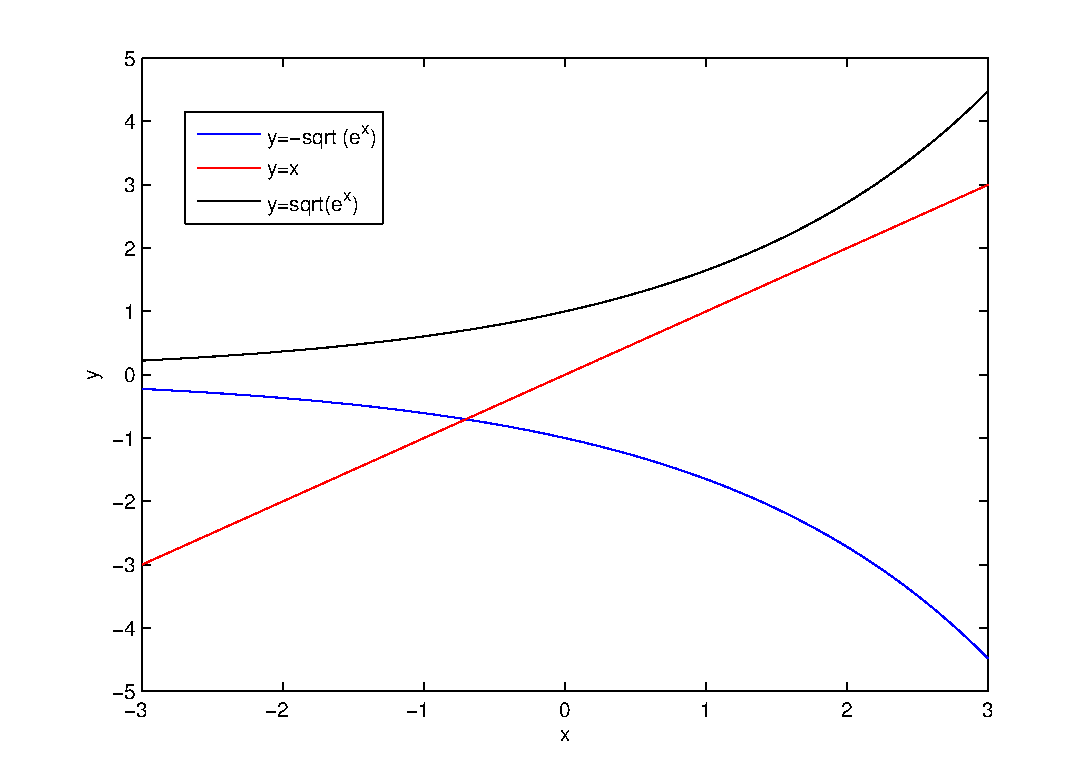
\includegraphics[width=14cm]{pfijo1.pdf}
\bicaption{$g(x)=\pm \sqrt{e^x}$, Solo la rama negativa tiene un punto fijo.}{$g(x)=\pm \sqrt{e^x}$, only negative branch has a fixed point.}
\label{fig:pfijo01}
\end{figure}

\begin{paracol}{2}
    
En nuestro ejemplo hemos obtenido tres formas distintas de \emph{despejar} la variable $x$. La cuestión que surge inmediatamente es, si todas las funciones obtenidas, tienen un punto fijo y, en caso de tenerlo, si es posible alcanzarlo iterativamente.

En el primer caso, $x=\pm \sqrt{e^x}$, obtenemos las dos ramas de la raíz cuadrada. Cada una de ellas constituye a los efectos de nuestro cálculo una función distinta. Si las dibujamos junto a la recta $y=x$ (figura \ref{fig:pfijo01}), observamos que solo la rama negativa la corta. Luego será  esta rama $g(x)=-\sqrt{e^x}$,  la que podremos utilizar para obtener la raíz de la función original por el método del punto fijo. La rama positiva, al no cortar a la recta $y=x$ en ningún punto, es una función que carece de punto fijo.

\switchcolumn
    
In our example we have obtained three different ways of \emph{clearing} the variable $x$. The question that immediately arises is whether all the functions obtained have a fixed point and, if so, whether it is possible to reach it iteratively.

In the first case, $x=\pm \sqrt{e^x}$, we obtain the two branches of the square root. For the purposes of our calculation, each of them constitutes a different function. If we draw them next to the straight line $y=x$ (figure \ref{fig:pfijo01}), we observe that only the negative branch cuts it. Then it will be this branch $g(x)=-$-$sqrt{e^x}$, which we will be able to use to obtain the root of the original function by the fixed point method. The positive branch, as it does not cut the straight line $y=x$ at any point, is a function without a fixed point.

\switchcolumn
No es difícil demostrar, que la función $g(x)=-\sqrt{e^x} $ cumple las condiciones del teorema de punto fijo descrito más arriba para el intervalo $(-\infty, 0]$. Luego el algoritmo del punto fijo debería converger para cualquier punto de inicio $x_0$ contenido en dicho intervalo. De hecho, para esta función, el algoritmo converge desde cualquier punto de inicio (Si empezamos en punto positivo, el siguiente punto, $x_1$ será negativo, y por tanto estará dentro del intervalo de convergencia). Esta función es un ejemplo de que el teorema suministra una condición suficiente, pero no necesaria para que un punto fijo sea atractivo. 
\switchcolumn

It is not difficult to show that the function $g(x)=-\sqrt{e^x}$ satisfies the conditions of the fixed point theorem described above for the interval $(-\infty, 0]$. Then the fixed point iteration should converge for any starting point $x_0$ contained in that interval. In fact, for this function, the algorithm converges from any starting point. (If we start at a positive point, the next point, $x_1$ will be negative, and therefore within the interval of convergence). This function is an example of the theorem providing a sufficient, but not necessary condition for a fixed point to be attractive. 

\switchcolumn

La figura \ref{fig:pfijo2} muestra un ejemplo del cálculo de la raíz de la función $f(x)=e^x-x^2$ empleando la función $g(x)=-\sqrt{e^x}$, para obtener el punto fijo. Se ha tomado como punto de partida $x_0=2.5$, un valor fuera del intervalo en el que se cumple el teorema. Como puede observarse en \ref{fig:pfijo21}. A pesar de ello el algoritmo converge rápidamente, y tras 5 iteraciones, \ref{fig:pfijo25}, ha alcanzado el punto fijo ---y por tanto la raíz buscada---, con la tolerancia impuesta.

\switchcolumn

Figure \ref{fig:pfijo2} shows an example of the calculation of the root of the function $f(x)=e^x-x^2$ using the function $g(x)=-\sqrt{e^x}$, to obtain the fixed point. We have taken as a starting point $x_0=2.5$, a value outside the interval in which the theorem is satisfied. As can be seen in \ref{fig:pfijo21}. In spite of this, the algorithm converges quickly, and after 5 iterations, \ref{fig:pfijo25}, has reached the fixed point ---and therefore the root sought---, with the imposed tolerance.

\end{paracol}

%TODO REvisar ESTA FIGURA
\begin{figure}[h]
\centering
\subfigure[valor inicial\label{fig:pfijo21}]{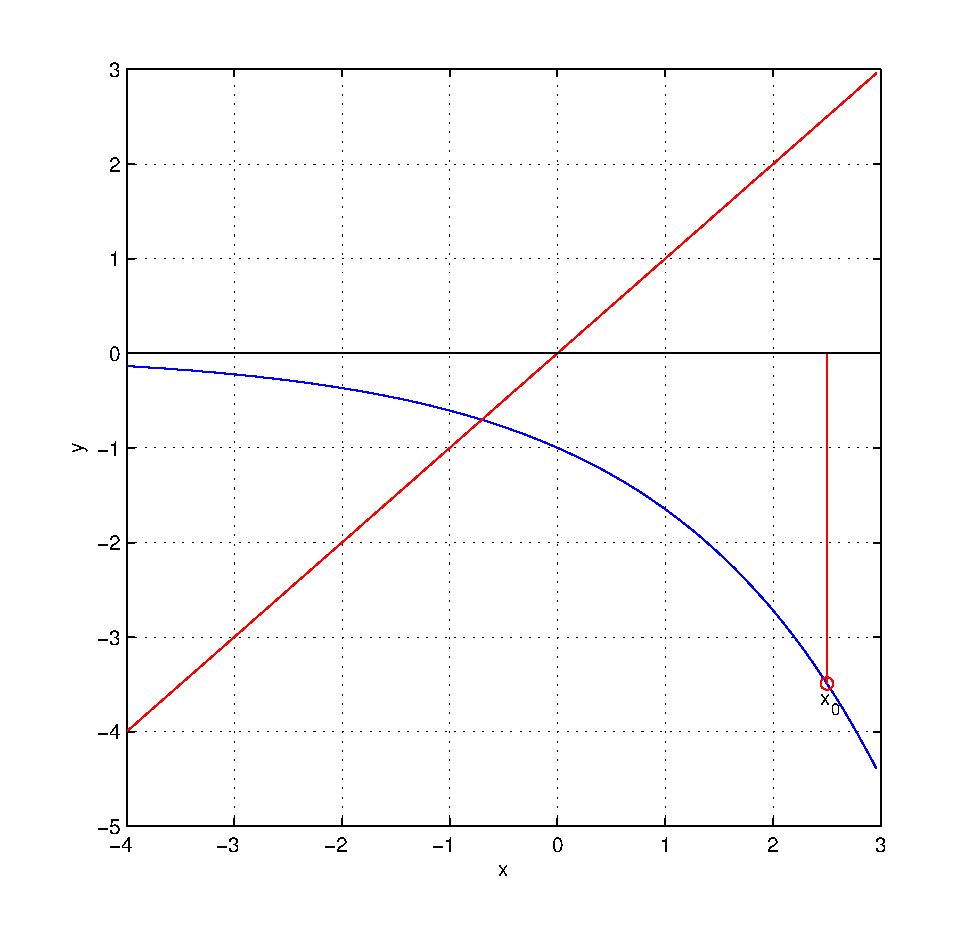
\includegraphics[height=5.5cm]{pfijo3.pdf}} \qquad
\subfigure[iteracion 1]{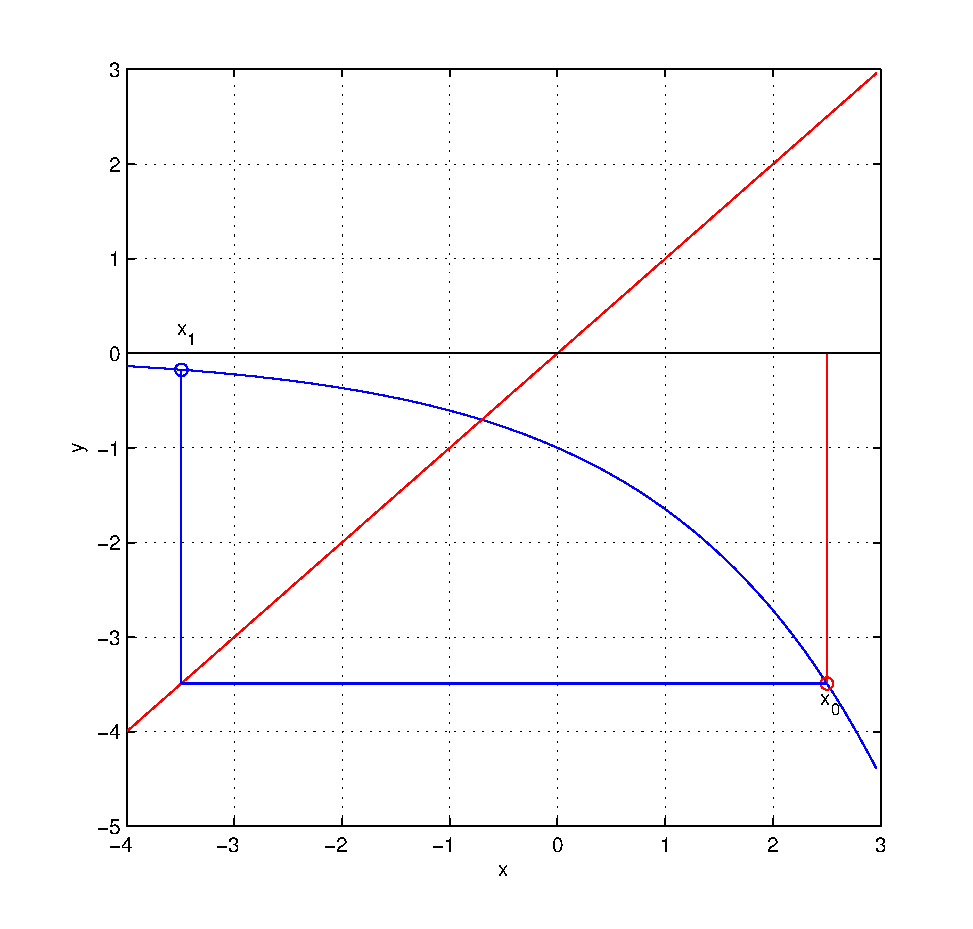
\includegraphics[height=5.5cm]{pfijo4.pdf}}\\
\subfigure[iteración 2]{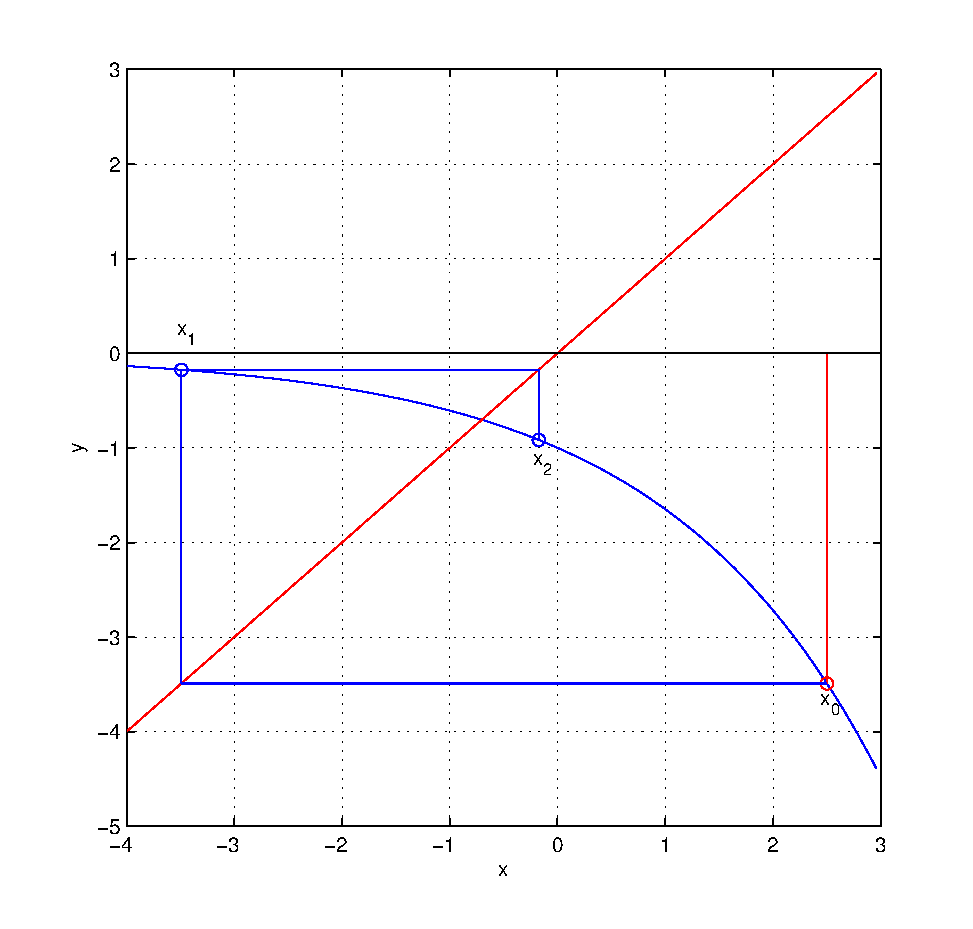
\includegraphics[height=5.5cm]{pfijo5.pdf}}\qquad
\subfigure[iteración 3]{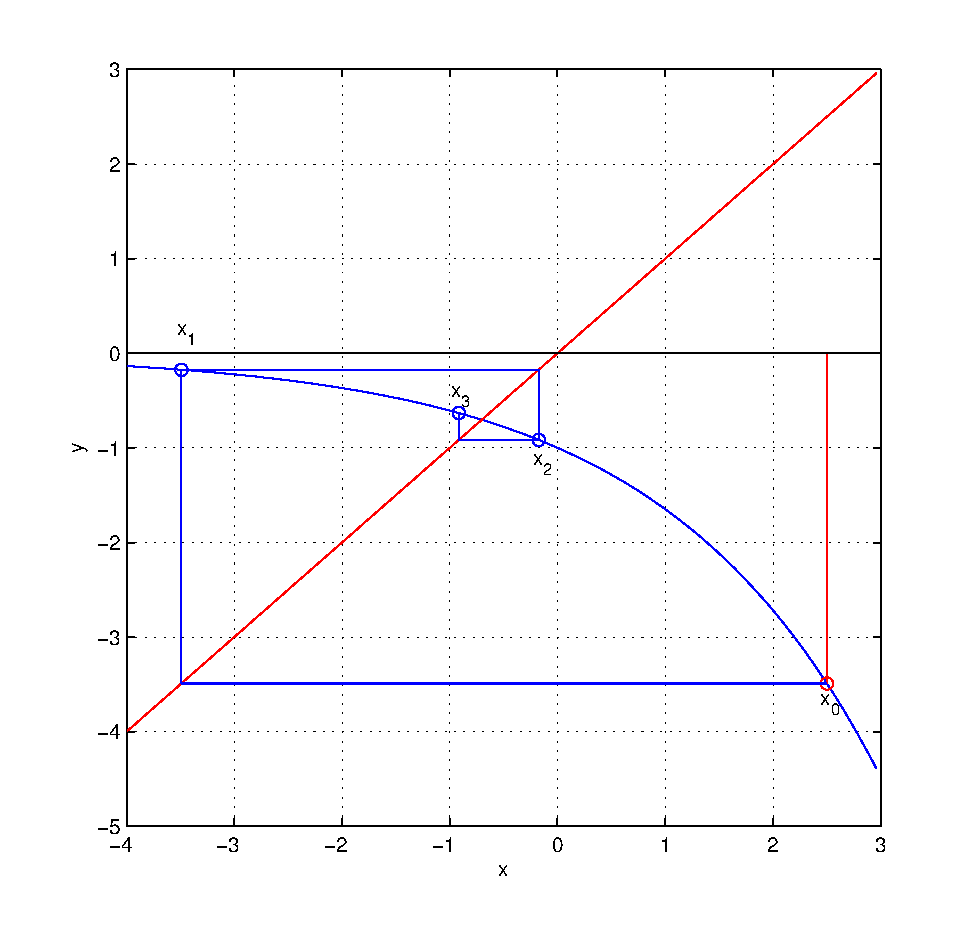
\includegraphics[height=5.5cm]{pfijo6.pdf}}\\
\subfigure[iteración 4]{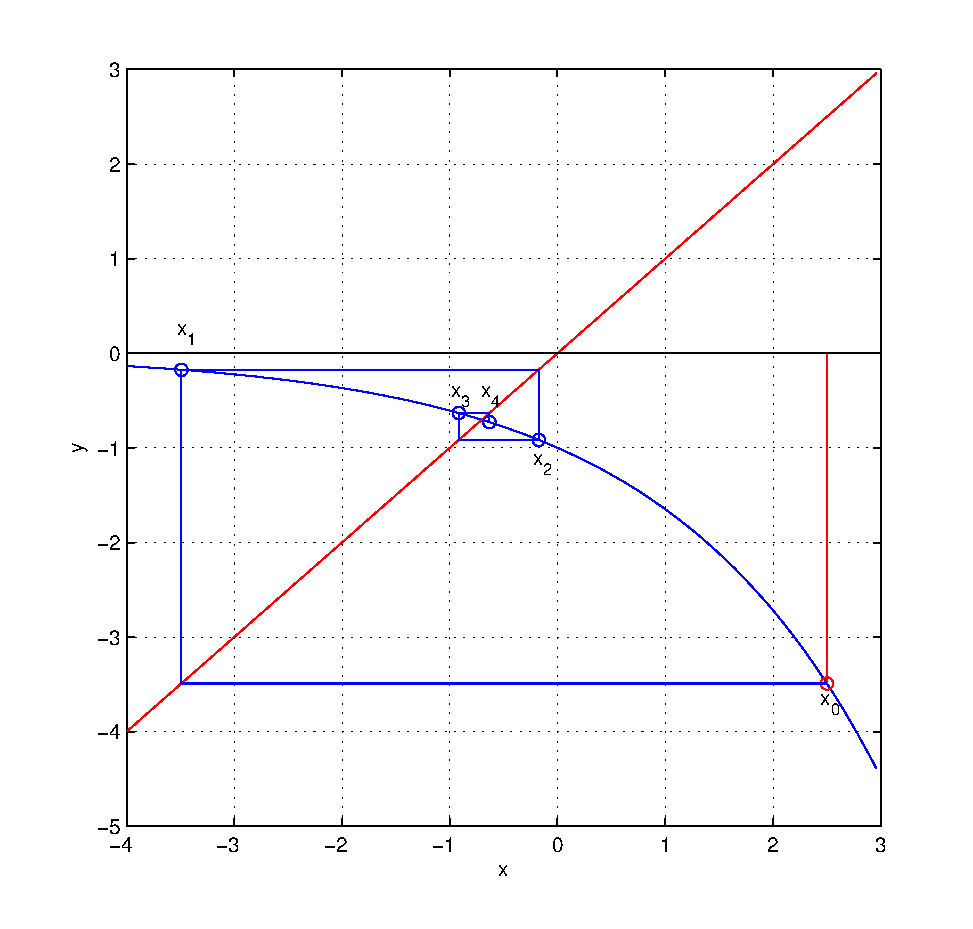
\includegraphics[height=5.5cm]{pfijo7.pdf}}\qquad
\subfigure[iteración 5 \label{fig:pfijo25}]{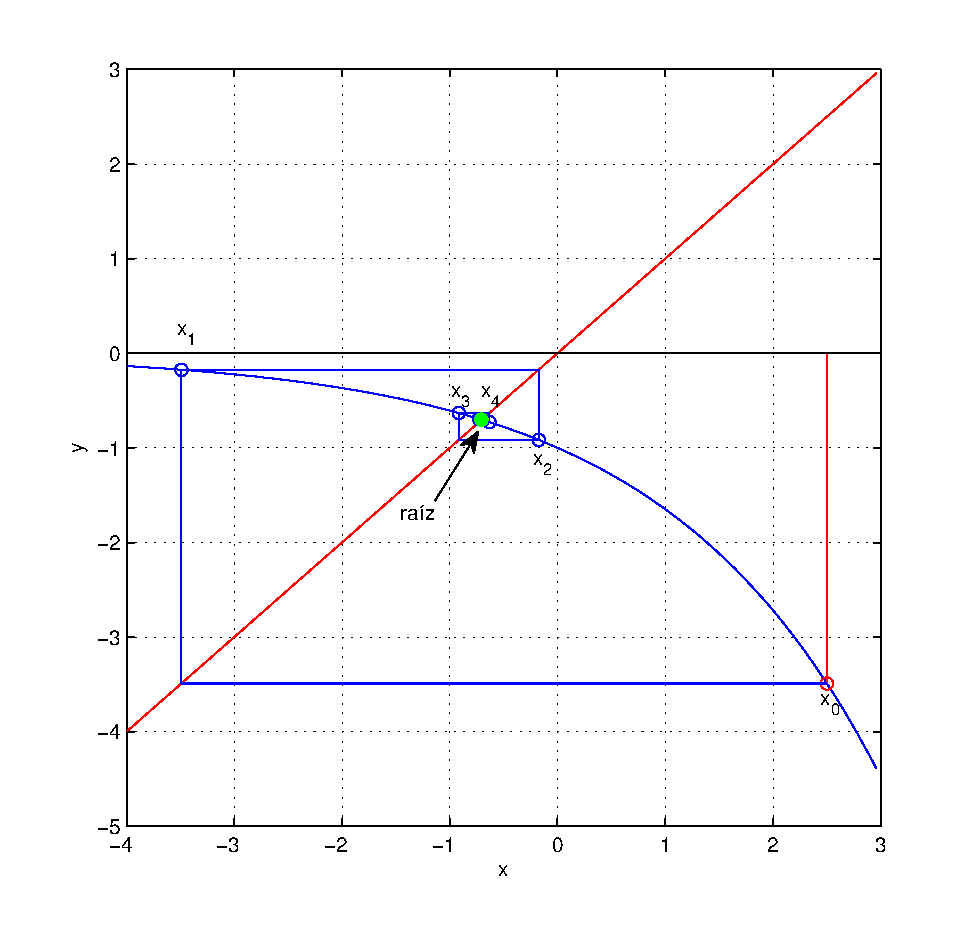
\includegraphics[height=5.5cm]{pfijo8.pdf}}

\bicaption{proceso de obtención de la raíz de la función $f(x)=e^x-x^2$ aplicando el método del punto fijo sobre la función $g(x)=-\sqrt{e^x}$}{Fixed point iteration to compute the root of $f(x)=e^x-x^2$ using the function $g(x)=-\sqrt{e^x}$}
\label{fig:pfijo2}
\end{figure}

\begin{paracol}{2}
    
Si tratamos de emplear la función $g(x)=ln(x^2)$ para obtener la raíz, observamos que la función no cumple el teorema para ningún intervalo que contenga la raíz. 

La figura \ref{fig:pfijo03} muestra la función $g(x)$, la recta $y=x$ y la evolución del algoritmo tras cuatro evaluaciones. Es fácil deducir que el algoritmo saltará de la rama positiva a la negativa y de ésta volverá a saltar de nuevo a la positiva. 

\switchcolumn

If we try to use the function $g(x)=ln(x^2)$ to obtain the root, we observe that the function does not satisfy the theorem for any interval containing the root. 

Figure \ref{fig:pfijo03} shows the function $g(x)$, the line $y=x$ and the evolution of the algorithm after four evaluations. It is easy to deduce that the algorithm will jump from the positive branch to the negative branch and from the negative branch back to the positive branch.

\end{paracol}

\begin{figure}[h]
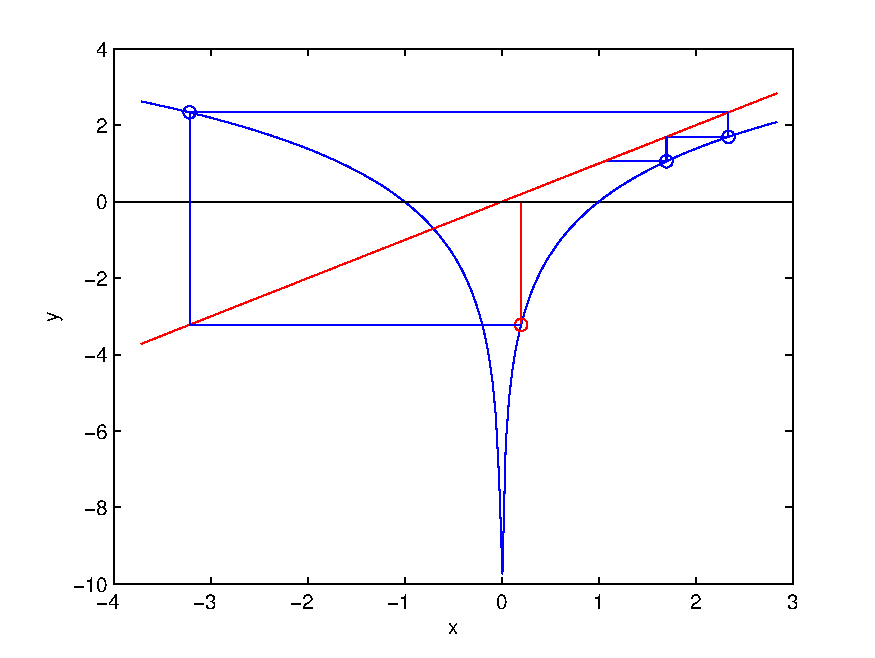
\includegraphics[width=14cm]{p1fijo0.pdf}
\bicaption{primeras iteraciones de la obtención de la raíz de la función $f(x)=e^x-x^2$ aplicando el método del punto fijo sobre la función $g(x)=ln(x^2)$.} {first iterations of obtaining the root of the function $f(x)=e^x-x^2$ by applying the fixed point method on the function $g(x)=ln(x^2)$.}
\label{fig:pfijo03}
\end{figure}

\begin{paracol}{2}
La función presenta una asíntota vertical en el $0$. Si se empieza desde $x_0=0$, $x_0=1$ 0 $x_0=-1$ el algoritmo no converge, puesto que la función diverge hacia $-\infty$. Para el resto de los valores, la función oscila entre una rama y otra. Si en alguna de las oscilaciones acierta a pasar suficientemente cerca del punto fijo, $x_n-x_{n-} \leq tol$, el algoritmo habrá aproximado la raíz, aunque propiamente no se puede decir que converja.

 La figura \ref{fig:pfijo41}, muestra la evolución del algoritmo, tomando como punto inicial $x_0=-0.2$.  Tras 211 iteraciones el algoritmo 'atrapa la raíz'. En este caso la tolerancia se fijó en $tol=0.01$.  
 
 \switchcolumn
 The function has a vertical asymptote at $0$. If one starts from $x_0=0$, $x_0=1$ 0 $x_0=-1$ the algorithm does not converge, since the function diverges towards $-\infty$. For the rest of the values, the function oscillates between one branch and another. If in any of the oscillations it manages to pass close enough to the fixed point, $x_n-x_{n-} \leq tol$, the algorithm will have approximated the root, although it cannot properly be said to converge.

 Figure \ref{fig:pfijo41}, shows the evolution of the algorithm, taking $x_0=-0.2$ as the starting point. After 211 iterations the algorithm 'catches the root'. In this case the tolerance was set to $tol=0.01$.

  \switchcolumn
  
 La gráfica \ref{fig:pfijo42} muestra una ampliación de \ref{fig:pfijo41} en la que pueden observarse en detalles los valores obtenidos para las dos últimas iteraciones. Las dos líneas horizontales de puntos marcan los límites $\text{raíz}\pm tol$. 
 
 El algoritmo se detiene porque la diferencia entre los valores obtenidos en las dos últimas iteraciones caen dentro de la tolerancia. El valor obtenido en la penúltima iteración, que proviene de la rama positiva de la función $g(x)$ cae muy cerca del punto fijo. El último valor obtenido, se aleja de hecho del valor de la raíz, respecto al obtenido en la iteración anterior, pero no lo suficiente como para salirse de los límites de la banda marcada por la tolerancia. Como resultado, se cumple la condición de terminación y el algoritmo se detiene.  
 
 Si disminuimos el valor de la tolerancia, no podemos garantizar que el algoritmo converja. De hecho, si trazamos cuales habrían sido los valores siguientes que habría tomado la solución del algoritmo, caso de no haberse detenido, es fácil ver que se alejan cada vez más de la raíz.  De nuevo habrá que esperar a que cambie de rama y vuelva  a pasar otra vez cerca del punto fijo para que haya otra oportunidad de que el algoritmo \emph{atrape} la solución.
 
  La gráfica \ref{fig:pfijo43} muestra la evolución del error en función del número de iteración. Como puede observarse, el error oscila de forma caótica de una iteración a la siguiente. De hecho, el estudio de las sucesiones de la forma $x_{n+1}=g(x_n)$ constituyen uno de los puntos de partidas para la descripción y el análisis de los llamados sistemas caóticos. 

Uno sencillo, pero muy interesante es el de la ecuación logística discreta, $x_{n+1}=R\cdot (1-x_n)\cdot x_n$. Esta ecuación muestra un comportamiento muy distinto, según cual sea el valor de $R$ y el valor inicial $x_0$ con el que empecemos a iterar.
  
\switchcolumn

The graph \ref{fig:pfijo42} shows an enlargement of \ref{fig:pfijo41} in which the values obtained for the last two iterations can be seen in detail. The two horizontal dotted lines mark the $text{root}\pm tol$. 

 The iteration stops because the difference between the values obtained in the last two iterations is lower than the tolerance. The value obtained in the penultimate iteration, which comes from the positive branch of the function $g(x)$, falls very close to the fixed point. The last value obtained, in fact, moves away from the value of the root, with respect to that obtained in the previous iteration, but not enough to fall outside the limits of the band marked by the tolerance. As a result, the termination condition is met and the algorithm stops. 

 If we decrease the value of the tolerance, we cannot guarantee that the algorithm will converge. In fact, if we plot what would have been the next values that the solution of the algorithm would have taken, had it not stopped, it is easy to see that they move further and further away from the root. Again, we will have to wait for it to change branches and pass close to the fixed point again for there to be another chance for the algorithm to catch the solution.
 
The graph \ref{fig:pfijo43} shows the evolution of the error as a function of the iteration number. As can be seen, the error oscillates chaotically from one iteration to the next. In fact, the study of sequences of the form $x_{n+1}=g(x_n)$ is one of the starting points for the description and analysis of so-called chaotic systems. 

A simple, but very interesting one is that of the discrete logistic equation, $x_{n+1}=R\cdot (1-x_n)\cdot x_n$. This equation shows very different behaviour, depending on the value of $R$ and the initial value $x_0$ with which we start iterating.
\end{paracol} 

\begin{figure}[h]
\centering
\subfigure[Evolución del algoritmo durante 211 iteraciones \label{fig:pfijo41}]{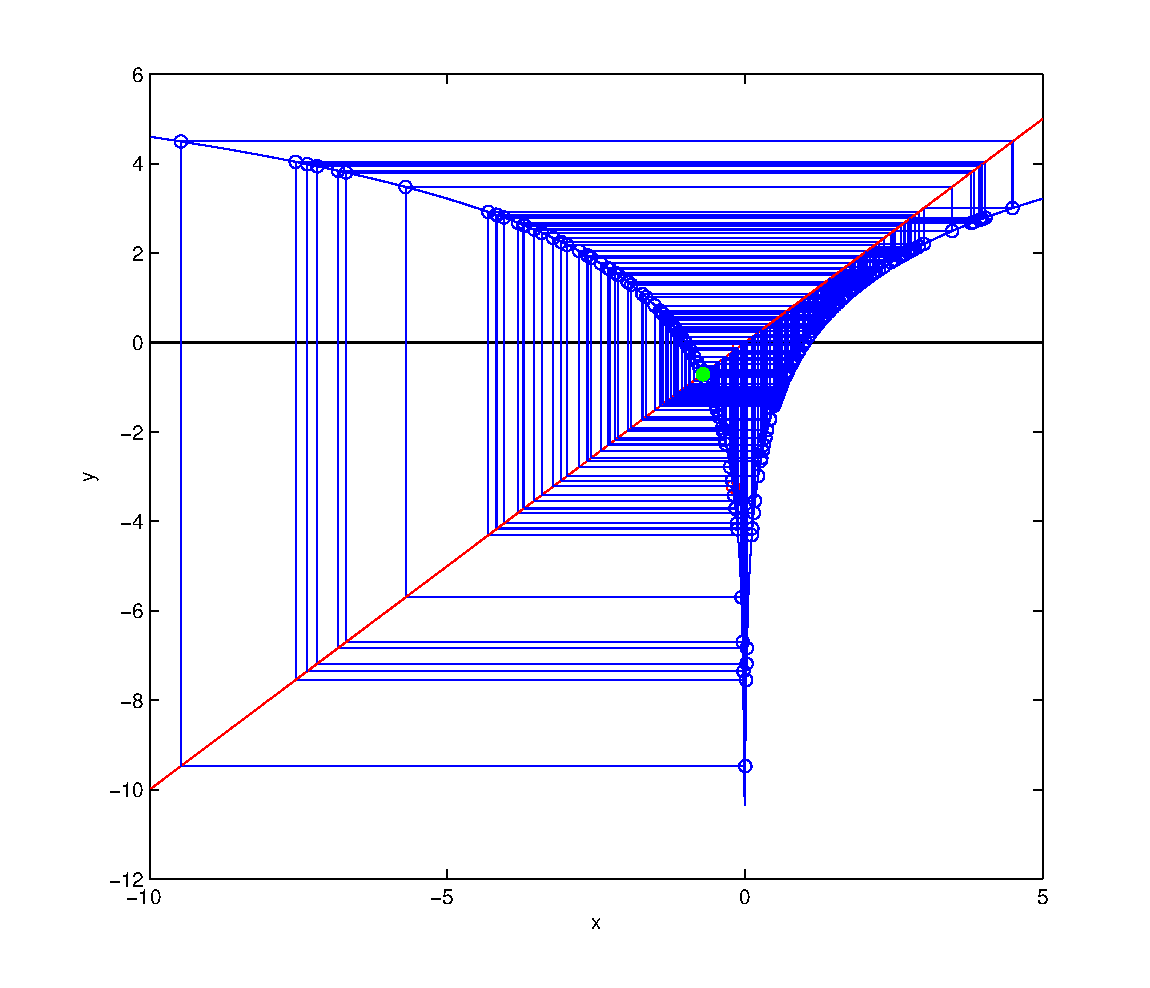
\includegraphics[width=7cm]{p2fijo1.pdf}} \qquad
\subfigure[Vista detallada de las ultimas iteraciones de \ref{fig:pfijo41} \label{fig:pfijo42}]{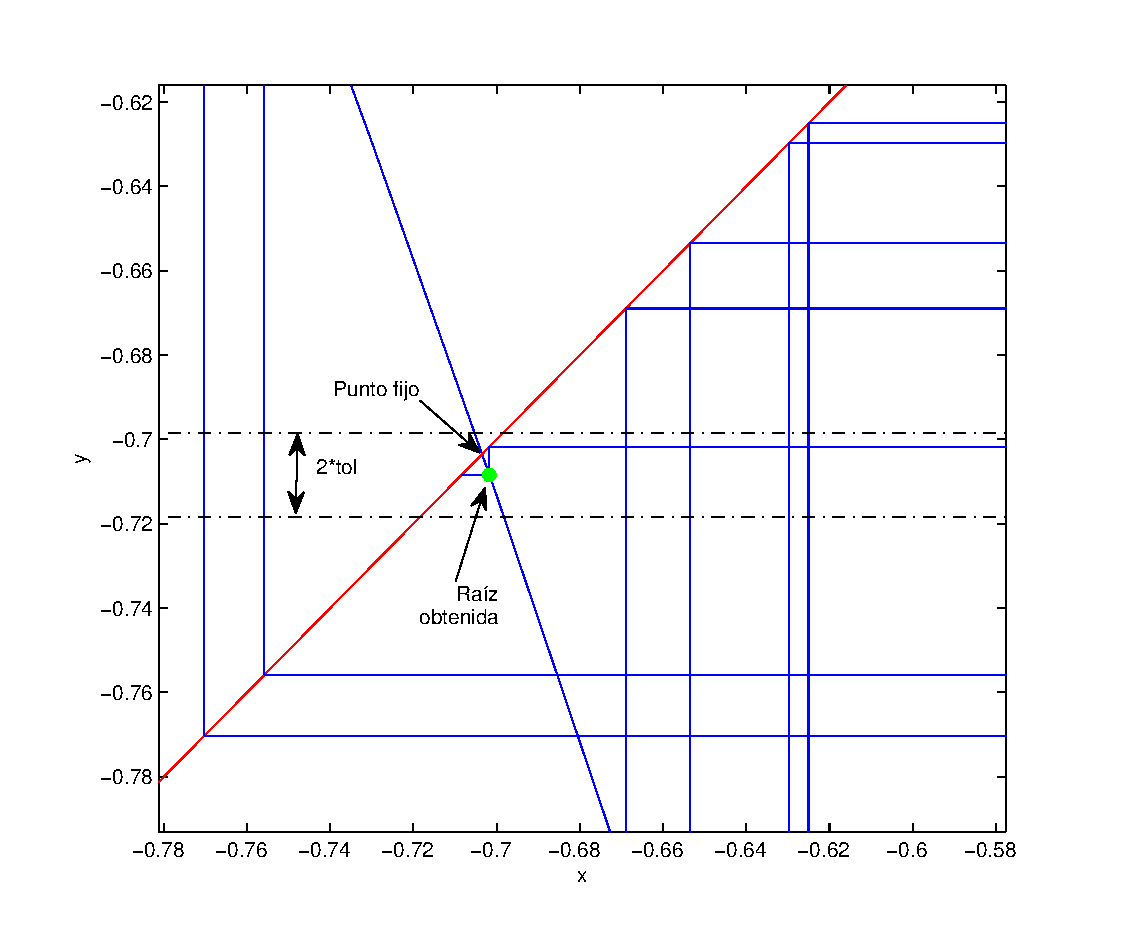
\includegraphics[width=7cm]{p2fijo1d2.eps}}\\
\subfigure[Evolución del error \label{fig:pfijo43}]{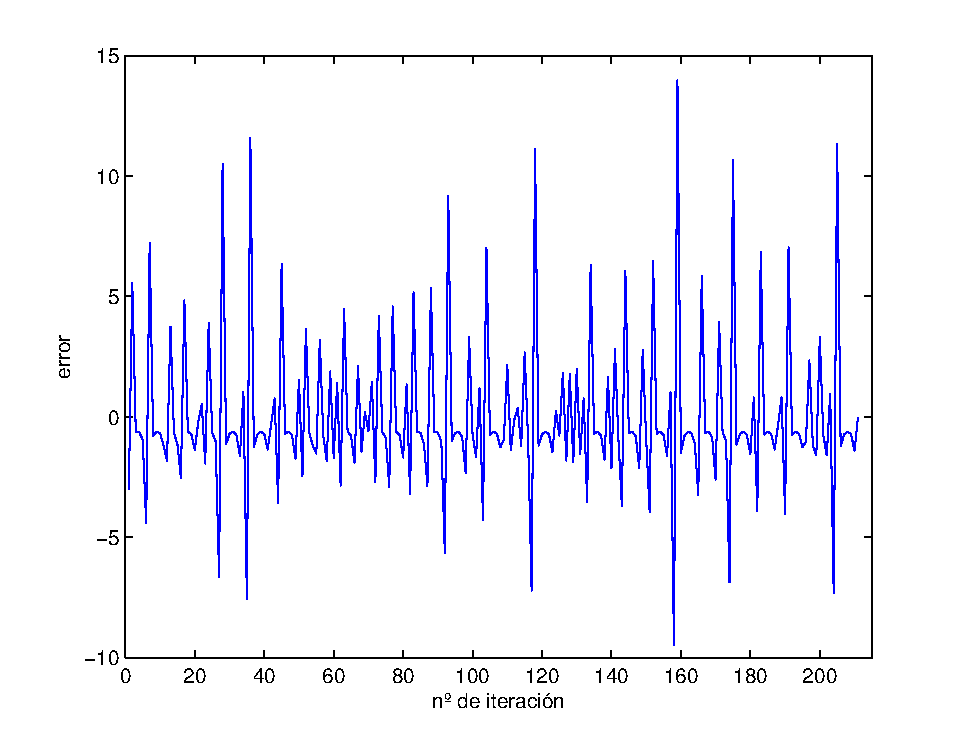
\includegraphics[width=7.2cm]{p2fijo1e.pdf}}

\bicaption{proceso de obtención de la raíz de la función $f(x)=e^x-x^2$ aplicando el método del punto fijo sobre la función $g(x)=ln(x^2)$, el método oscila sin converger a la solución.}{Fixed point iteration to compute the root of function $f(x)=e^x-x^2$ using the function $g(x)=ln(x^2)$, iteration oscillates without converging to the solution.}
\label{fig:pfijo4}
\end{figure}

\begin{paracol}{2}
Por último, si empleamos la función $g(x)=\frac{e^x}{x}$, no se cumple el teorema de punto fijo en ningún punt. En este caso, el algoritmo diverge siempre.  La figura \ref{fig:pfijo5} muestra la evolución del algoritmo del punto fijo para esta función. Se ha elegido un punto de inicio $x_0=-0.745$, muy próximo al valor de la raíz, para poder observar la divergencia de las soluciones obtenidas con respecto al punto fijo. Como puede verse, el valor de $x_n$ cada vez se aleja más de la raíz. LA solución oscila entre un valor que cada vez se aproxima más a cero y otro que tiende hacia $-\infty$. Si se deja aumentar suficientemente el número de iteraciones, llegará un momento en que se producirá un error de desbordamiento. 

A diferencia de lo que sucedía en la elección de $g(x)=ln(x^2)$, en este caso, el algoritmo no oscila entre las dos ramas. Si empezamos en la rama de la derecha, eligiendo un valor positivo para $x_0$, el algoritmo diverge llevando las soluciones hacia $+\infty$. Es un resultado esperable, ya que dicha rama no tiene ningún punto fijo.

\switchcolumn

Finally, if we use the function $g(x)=\frac{e^x}{x}$, the fixed point theorem is not satisfied at any point. In this case, the algorithm always diverges. Figure \ref{fig:pfijo5} shows the evolution of the fixed-point iteration for this function. A starting point $x_0=-0.745$, very close to the value of the root, has been chosen in order to observe the divergence of the solutions obtained with respect to the fixed point. As can be seen, the value of $x_n$ moves further and further away from the root. The solution oscillates between a value that gets closer and closer to zero and another that tends towards $-\infty$. If the number of iterations is allowed to increase sufficiently, there will come a time when an overflow error will occur. 

Unlike in the choice of $g(x)=ln(x^2)$, in this case, the algorithm does not oscillate between the two branches. If we start on the right-hand branch, choosing a positive value for $x_0$, the algorithm diverges, taking the solutions towards $+\infty$. This is to be expected, since this branch has no fixed point.

\end{paracol}


\begin{figure}
\centering
\subfigure[valor inicial]{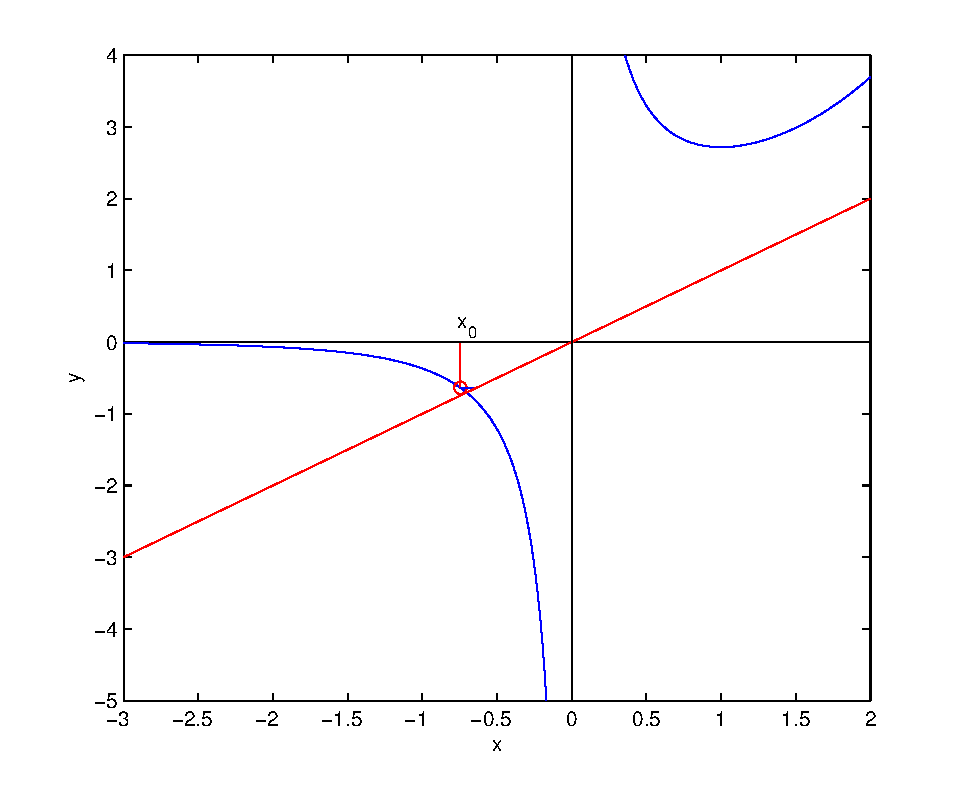
\includegraphics[width=7cm]{p3fijo0.pdf}} \qquad
\subfigure[iteracion 1]{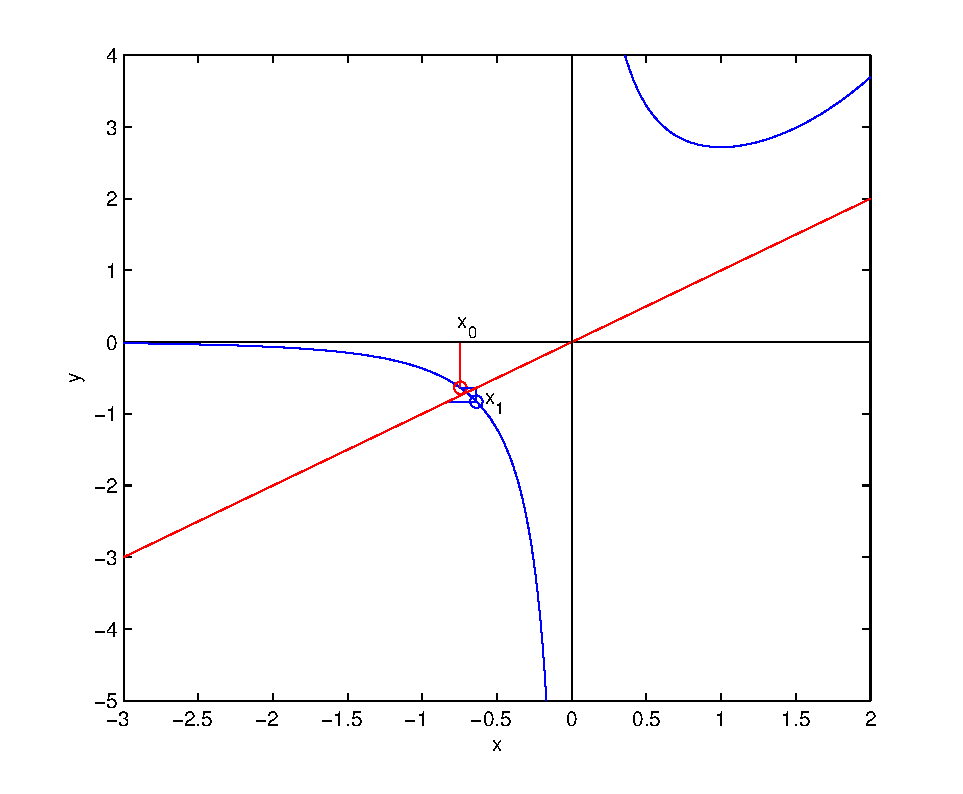
\includegraphics[width=7cm]{p3fijo1.pdf}}\\
\subfigure[iteración 2]{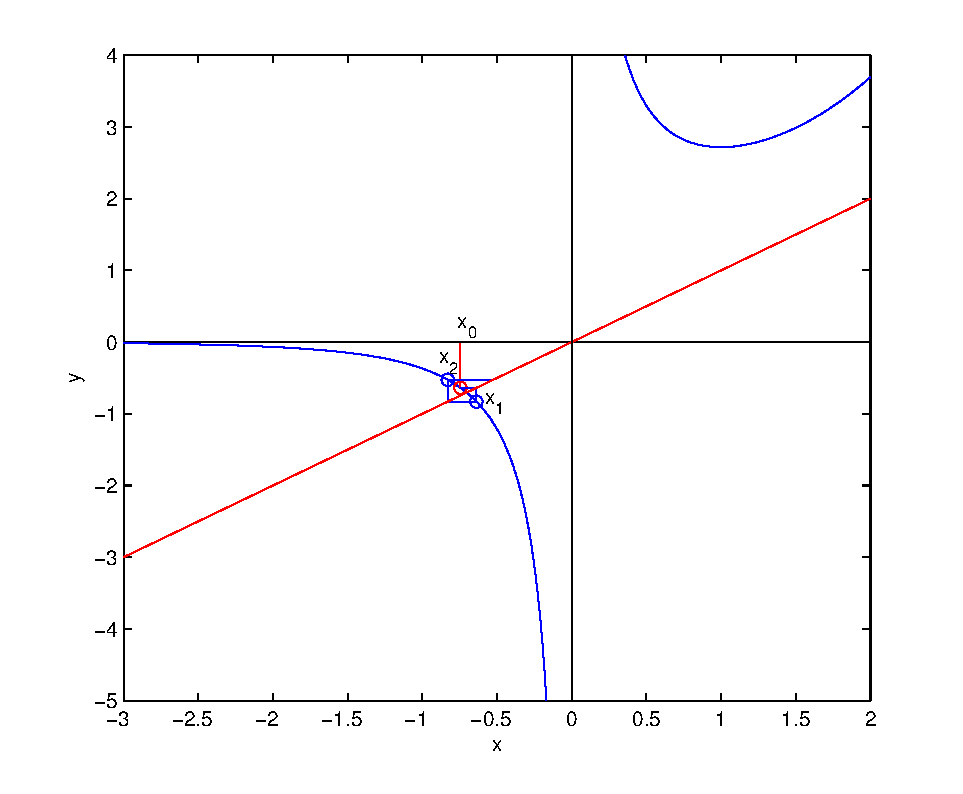
\includegraphics[width=7cm]{p3fijo2.pdf}}\qquad
\subfigure[iteración 3]{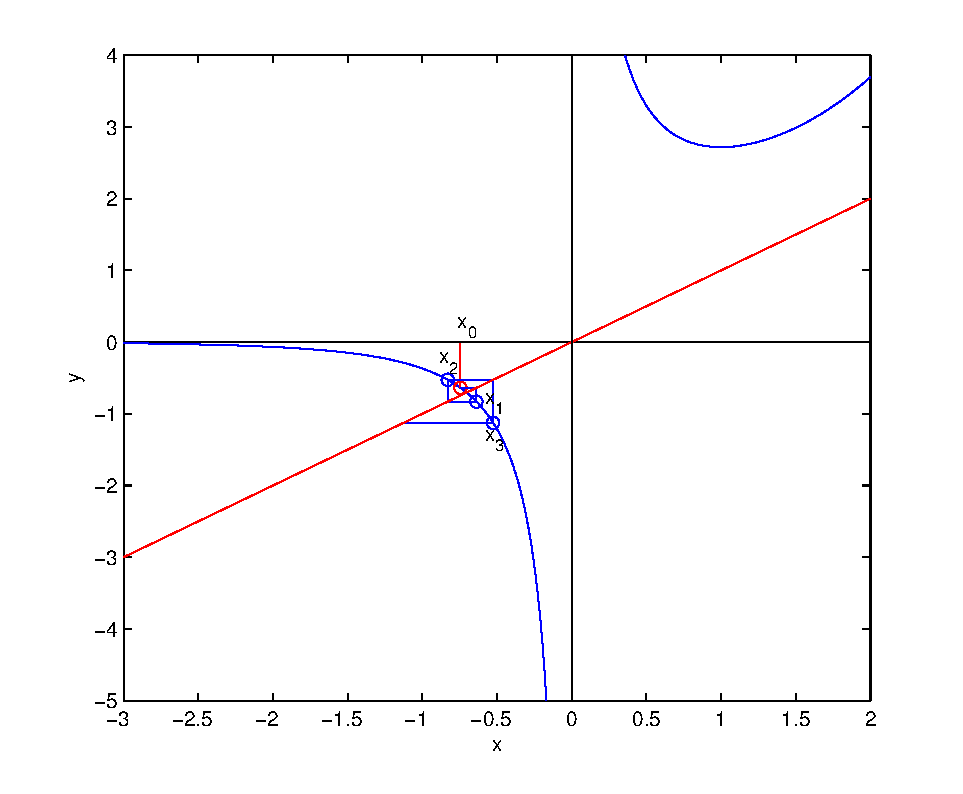
\includegraphics[width=7cm]{p3fijo3.pdf}}\\
\subfigure[iteración 4]{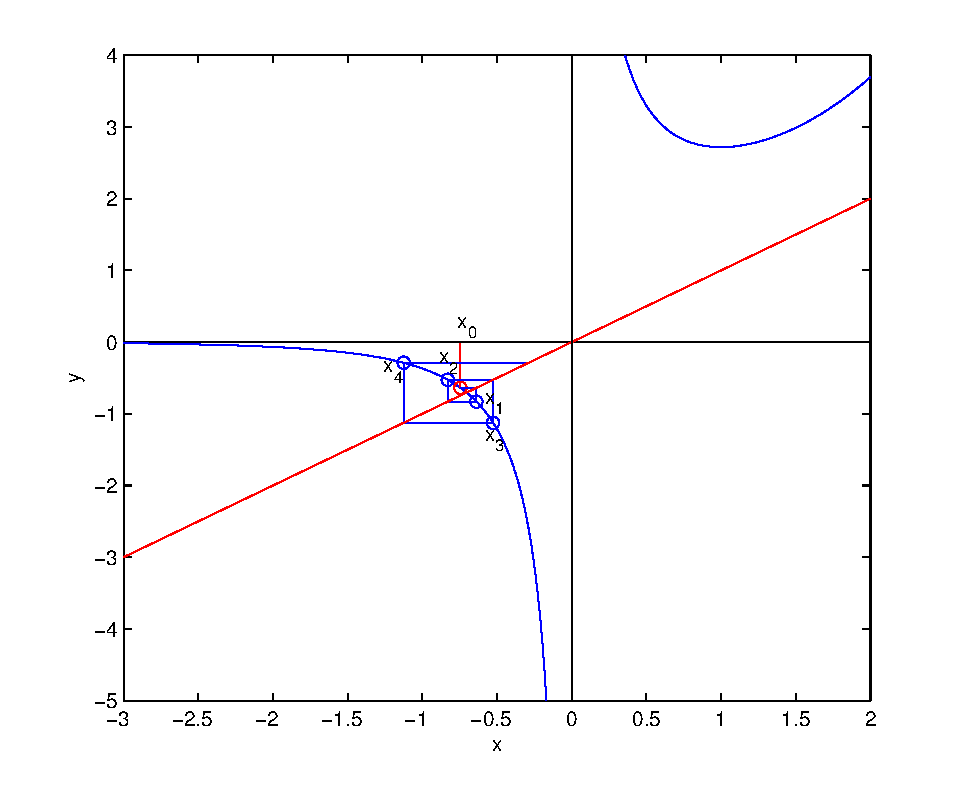
\includegraphics[width=7cm]{p3fijo4.pdf}}\qquad
\subfigure[iteración 5]{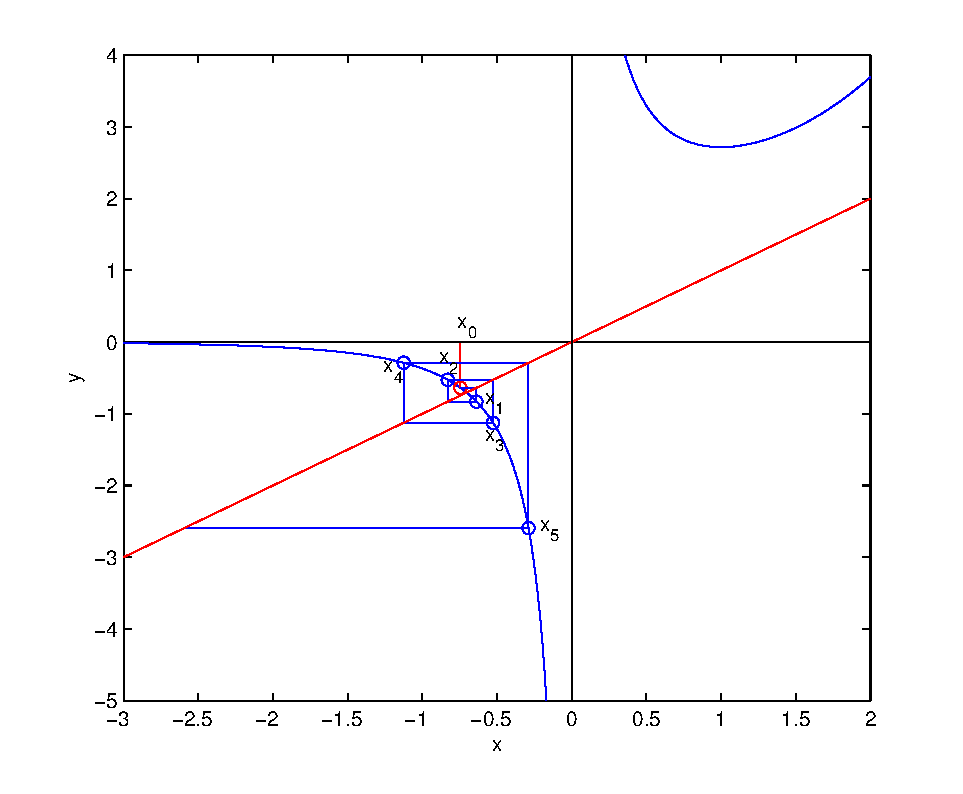
\includegraphics[width=7cm]{p3fijo5.pdf}}

\bicaption{proceso de obtención de la raíz de la función $f(x)=e^x-x^2$ aplicando el método del punto fijo sobre la función $g(x)=\frac{e^x}{x}$, el método diverge rápidamente.}{fixed point iteration to compute the root of function $f(x)=e^x-x^2$ using the function  $g(x)=\frac{e^x}{x}$, the iteration diverges quickly.}
\label{fig:pfijo5}
\end{figure}
\begin{paracol}{2}

\section{Cálculo de raíces de funciones con Python.}

Python tiene sus propios métodos para calcular raíces de funciones. Vamos a ver dos de esos métodos. Primero la función  \texttt{fsolve} del paquete \texttt{scipy.optimize} que calcula raices de todo tipo de funciones. Después veremos las funciones específicas para usar polinomios del paquete \texttt{numpy} y entre ellas la función \texttt{roots} para hallar las raices de un polinomio.

\switchcolumn

\section{Python root finding}

Python has its own methods for calculating roots of functions. Let's take a look at two of those methods. First, the \texttt{fsolve} function from the \texttt{scipy.optimize} package calculates roots of all kinds of functions. Then we will look at the specific functions for using polynomials from the \texttt{numpy} package, including the \texttt{roots} function for finding the roots of a polynomial.

\subsection{Function \texttt{fsolve}}

\switchcolumn

\subsection{La función \texttt{fsolve}}

La función \texttt{fsolve} se encuentra en el paquete \texttt{optimize} de \texttt{scipy}. Esta función devuelve las raices de un sistema de ecuaciones definidas por $func(x)=0$ dado un punto de inicio.

Si el algoritmo no llega a converger \texttt{fsolve} devuelve el resultado de la última iteración.

\switchcolumn
\texttt{fsolve} returns the roots of the (non-linear) equations defined by $func(x) = 0$ given a starting estimate.

If algorithm fails \texttt{fsolve} returns the last iteration result.

\switchcolumn

La sintaxis del método \texttt{fsolve} en su forma más sencilla es la siguiente:

\begin{minted}{python}
 import scipy.optimize as opt

 roots=opt.fsolve(fun,[x0])    
\end{minted}


donde \texttt{fun} representa el nombre de la función que se desea evaluar, \texttt{[x0]}, son los valores de partida de las raices  y \texttt{roots} las raices calculadas oir \texttt{fsolve}. 

\switchcolumn
The syntax of the \texttt{fsolve} method in its simplest form is as follows:

\begin{minted}{python}
 import scipy.optimize as opt

 roots=opt.fsolve(fun,[x0])
\end{minted}

where \texttt{fun} represents the name of the function to be evaluated, \texttt{[x0]} are the starting values of the roots and \texttt{roots} are the calculated roots or \texttt{fsolve}.

\switchcolumn

Un ejemplo de uso de \texttt{fsolve} para calcular la raiz de $f(x)=e^x-x^2$ partiendo de una aproximación inicial de $x_0=2$ sería el siguiente:

\begin{minted}{python}
import numpy as np
import scipy.optimize as opt

def fun(x):
    y=np.exp(x)-x**2
    return y

roots=opt.fsolve(fun,-2)

\end{minted}

El método \texttt{fsolve}, tiene muchas posibilidades de ajuste de la precisión, el número máximo de iteraciones, etc. Para obtener una visión mas completa de su uso, consultar la ayuda de \texttt{scipy.optimize.fsolve}.

\switchcolumn
An example of using \texttt{fsolve} to calculate the root of $f(x)=e^x-x^2$ starting from an initial approximation of $x_0=2$ would be as follows:

\begin{minted}{python}
import numpy as np
import scipy.optimize as opt

def fun(x):
    y=np.exp(x)-x**2
    return y

roots=opt.fsolve(fun,-2)

\end{minted}

The \texttt{fsolve} method has many possibilities to adjust the precision, the maximum number of iterations, etc. For a more complete overview of its use, see the \texttt{scipy.optimize.fsolve} help.

\end{paracol}


\begin{paracol}{2}
\subsection{Cálculo de raíces de polinomios.} \index{Polinomios}

Podemos crear y manipular polinomios en NumPy usando las clases del paquete\\ \texttt{numpy.polynomial package} incorporado en Numpy 1.4. La clase \texttt{Polynomial} proporciona los métodos numéricos habituales en Python $+$, $-$, $*$, $/$, $\%$ y otros específicos de polinomios.

Para crear un polinomio tendremos que importar el módulo \texttt{numpy.polynomial} y usar la clase \texttt{Polynomial}. A esta clase, como primer argumento le proporcionarenmos un vector cuyos elementos, son los coeficientes del polinomio ordenados de  menor grado a mayor grado. Así por ejemplo, el polinomio $y=1 + 4x + 3x^2+2x^3$ se representa mediante el vector, $[1\ 4\ 3\ 2]$ de la siguiente manera:

\switchcolumn

\subsection{Polynomials roots}
Polynomials in NumPy can be created, manipulated, and even fitted using the convenience classes of the \texttt{numpy.polynomial package}, introduced in NumPy 1.4. The Polynomial class provides the standard Python numerical methods $+$, $-$, $*$, $//$, $\%$, $**$ and others. 

To create a polynomial we have to import the polynomial package and use the Polynomial class. Coefficients are given in an array-like form in order of increasing degree, i.e., $p1=[1\ 4\ 3\ 2]$  give $y=1 + 4x + 3x^2+2x^3$.
\end{paracol}

\begin{minted}{python}
from numpy.polynomial import Polynomial as P
p = P([1,4,3,2])
\end{minted}

\begin{paracol}{2}
El polinomio $y=3x^4+2x^2+6x$ se representa mediante el vector,  $[0\ 6\ 2\ 0\ 3]$ y, en general, el polinomio $y(x)=a_0+a_1x+a_2x^2+\cdots+a_{n-1}x^{n-1}+ a_nx^n$  se representa mediante el vector $[a_0\ a_1\ a_2\  \cdots  a_{n-1}\ a_n]$. Si al polinomio le falta algún o algunos términos, el elemento correspondiente toma el valor $0$ en el vector que representa el polinomio.    

\switchcolumn

Polynomial $y=3x^4+2x^2+6x$ is represented by array,  $[0\ 6\ 2\ 0\ 3]$. In general, polynomial $y(x)=a_0+a_1x+a_2x^2+\cdots+a_{n-1}x^{n-1}+ a_nx^n$  is represented by array $[a_0\ a_1\ a_2\  \cdots  a_{n-1}\ a_n]$. if the polynomial does not have any of the monomials, the corresponding coefficient is array  is $0$.    

\end{paracol}


\begin{minted}{python}
from numpy.polynomial import Polynomial as P
p = P([0,6,2,0,3])
\end{minted}

\begin{paracol}{2}
\paragraph{El método \texttt{roots} de la clase \texttt{Polynomial}.} \index{Polinomios!Raíces de un polinomio} Este método de la clase \texttt{Polynomial} calcula las raíces de un polinomio de grado $n$ definido como un  como los que acabamos de describir. La sintaxis es: \texttt{p.roots()} donde  \texttt{p} es un polinomio definido como hemos visto antes. Veamos un ejemplo. Dado el polinomio $y(x)=x^3-6^2+11x-6$ lo expresaríamos y calcularíamos sus raices en python como,

\switchcolumn
\paragraph{Method \texttt{roots}.}\index{} This method returns the roots of a polynomial defined using the class \texttt{Polynomial}. The sintax is: \texttt{p.roots()} where \texttt{p} is a polynomial defined as above. Let's see an example. Given the polynomial  $y(x)=x^3-6^2+11x-6$ we define it and compute the roots in python as:
\end{paracol}

\begin{minted}{python}
from numpy.polynomial import Polynomial as P
p=P([1,-6,11,-6])
print(p)
print("The roots are:\t",p.roots())
\end{minted}
\begin{minted}{pycon}
1.0 - 6.0·x + 11.0·x² - 6.0·x³
The roots are:	 [0.33333333 0.5        1.        ]

\end{minted}

\begin{paracol}{2}
El método \texttt{roots} devuelve las raices del polinomio en un único vector. Si el polinomio tiene raices complejas devuelve su parte real como en el caso del polinomio  $y(x)=x^2+2x+1$

\switchcolumn
The method \texttt{roots} returns the polynomial roots in a single vector. If the polynomial has complex roots it returns its real part as in the case of the polynomial $y(x)=x^2+2x+1$
\end{paracol}

\begin{minted}{python}
from numpy.polynomial import Polynomial as P
p=P([1,2,1])
print(p)
print("The roots are:\t",p.roots())
\end{minted}
\begin{minted}{pycon}
1.0 + 2.0·x + 1.0·x²
The roots are:	 [-1.00000001 -0.99999999]
\end{minted}
\begin{paracol}{2}
\paragraph{La función \texttt{fromroots}.} Esta función podría considerarse la opuesta a la anterior; dado un vector que contiene las raíces de un polinomio, nos devuelve el polinomio correspondiente, Por ejemplo si definimos el vector de raíces, $[3,2,1]$ podemos obtener el polinomio que posee esas raices. En este caso el polinomio es $y(x)=x^3-6x^2+11x-6$

\switchcolumn

\paragraph{The method\texttt{fromroots}.}. This method could be considered the opposite of the previous one; given a vector containing the roots of a polynomial, it returns the corresponding polynomial. For example, if we define the vector of roots, $[3,2,1]$ we can obtain the polynomial that has those roots. In this case the polynomial is $y(x)=x^3-6x^2+11x-6$.

\end{paracol}
\begin{minted}{python}
from numpy.polynomial import Polynomial as P
p=P.fromroots([3,2,1])
print(p)
\end{minted}
\begin{minted}{pycon}
-6.0 + 11.0·x - 6.0·x² + 1.0·x³
\end{minted}
\begin{paracol}{2}
\paragraph{El método \texttt{linspace}.}
El método  \texttt{linspace} devuelve valores equiespaciados $x$ y sus correspondientes $y$ en el dominio definido del polinomio. Si dicho dominio no se ha definido al crear el polinomio, se establece por defecto como $[-1,1]$. Este método es muy útil para representar un polinomio gráficamente, como se ve en el siguiente ejemplo y en la figura \ref{fig:poly-linespace}.

\switchcolumn

\paragraph{Method \texttt{linspace}.}
Method \texttt{linspace} returns $x$, $y$ values at equally spaced points in domain of polynomial. If domain has been not defined $[-1,1]$ is set. This method is usefull to plot the polynomial, as in the next example and figure \ref{fig:poly-linespace}.

\end{paracol}

\begin{minted}{python}
from numpy.polynomial import Polynomial as P
#Polynomial p created and domain defined as [-2,2]
p=P([0,6,2,0,3],[-2,2])
dat=p.linspace()
plt.figure()
plt.grid()
plt.plot(dat[0],dat[1])
plt.xlabel('x')
plt.ylabel('y')
p_string=str(p)
plt.title(p_string)
\end{minted}

\begin{figure}
    \centering
    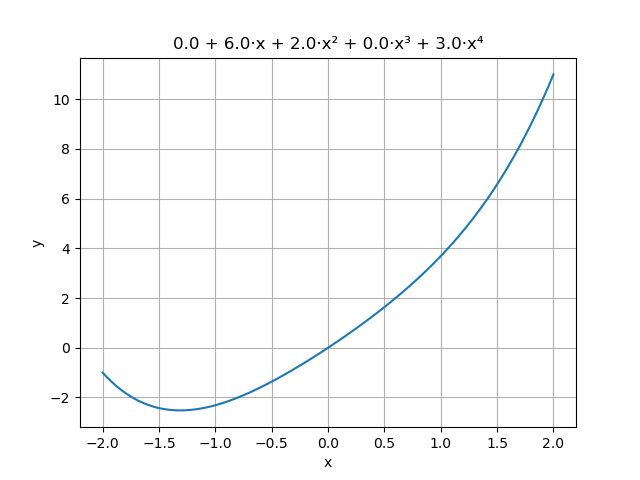
\includegraphics[width=0.5\linewidth]{figuras/poli_linspace.png}
    \bicaption{Polinomio dibujado usando \texttt{linspace}}{Plotting a polynomial using \texttt{linspace}}
    \label{fig:poly-linespace}
\end{figure}

\begin{paracol}{2}
\paragraph{El método \texttt{deriv}.}
El método \texttt{deriv} devuelve un polinomio que es el resultado de calcular la derivada del polinomio actual.

\switchcolumn
\paragraph{Method \texttt{deriv}.}
Returns a polynomial instance of that is the derivative of the current polynomial.

\switchcolumn
\paragraph{El método \texttt{integ}.}
Devuelve un polinomio que es la integral del polinomio actual.

\switchcolumn
\paragraph{Method \texttt{integ}.}
Returns a polynomial that is the integral of the current polynomial.

\switchcolumn
\paragraph{El método \texttt{copy}.}
Devuelve una copia del polinomio actual.
\switchcolumn
\paragraph{Method \texttt{copy}.}
Returns a copy of the current polynomial.
\end{paracol}

\begin{minted}{python}
from numpy.polynomial import Polynomial as P

#Create a polynomial with roots 3, -2, 2
p3=P.fromroots([3,-2,2])
print(p3)
#Compute the polynomial that is its derivative
pdot=p3.deriv()
print("Derivative:", pdot)
#Compute the polynomial that is the integral
pint=p3.integ()
print("Integral:", pint)
#Create polynomial p4 as a copy of pint
p4=pint.copy()
print(p4)
\end{minted}

\begin{minted}{pycon}
12.0 - 4.0·x - 3.0·x² + 1.0·x³
Derivative: -4.0 - 6.0·x + 3.0·x²
Integral: 0.0 + 12.0·x - 2.0·x² - 1.0·x³ + 0.25·x^4
0.0 + 12.0·x - 2.0·x² - 1.0·x³ + 0.25·x^4
\end{minted}

\begin{paracol}{2}
\section{Cálculo de raices con la precisión máxima}
Como ya se vio en la sección \ref{errn} todos los números que empleamos en un ordenador están sometidos a errores a causa del tamaño finito de los registros empleados para guardarlos. Cualquier número que queramos representar ha de aproximarse por un número máquina. Por lo tanto, en vez de buscar la aproximación a la raiz de una función con una tolerancia dada, podemos hallarla con la máxima precisión que nos permita la representación numérica empleada. Esta precisión máxima está relacionada con el \texttt{epsilon} del computador ya que la distancia entre dos números consecutivos es el épsilon multiplicado por dos elevado al exponente del número. De esta manera, por muchas iteraciones que hagamos la mejor aproximación que vamos a poder obtener de una raiz la obtendremos cuando el intervalo en el que se busca la raiz queda reducido a \texttt{eps} y por lo tanto no es posible reducirlo aún más. 

En \texttt{Numpy} el método \texttt{spacing(a)} nos devuelve la distancia entre $a$ y el siguiente número adyacente más próximo. De esta manera si a un número $x$ le sumamos un valor menor que \texttt{spacing(x)} el resultado es el mismo número. Hay que tener en cuenta que para números negativos $x<0$ la distancia que nos devuelve \texttt{spacing(x)} es también negativa. No debería haber ningún número máquina entre $x$y $x+spacing(x)$ para cualquier $x$ finito.

\switchcolumn
\section{Computing roots at maximum precision.}
As we saw in section \ref{errn} all the numbers we use in a computer are subject to errors because of the finite size of the registers used to store them. Any number we want to represent has to be approximated by a machine number. Therefore, instead of looking for the approximation to the root of a function with a given tolerance, we can find it with the maximum precision allowed by the numerical representation used. This maximum precision is related to the computer's epsilon, since the distance between two consecutive numbers is the epsilon multiplied by two raised to the exponent of the number. Thus, no matter how many iterations we make, the best approximation we will be able to obtain of a root will be when the interval in which the root is sought is reduced to \texttt{eps} and therefore it is not possible to reduce it further. 

In \texttt{Numpy} the method \texttt{spacing(a)} returns the distance between $a$ and the next nearest adjacent number. So if we add a value less than \texttt{spacing(x)} to a number $x$, the result is the same number. Note that for negative numbers $x<0$ the distance returned by \texttt{spacing(x)} is also negative. There should not be any representable number between $x + spacing(x)$ and $x$ for any finite $x$.

\end{paracol}  


\begin{minted}{pycon}
import numpy as np

np.spacing(1)
Out[9]: 2.220446049250313e-16

np.spacing(1e-10)
Out[10]: 1.2924697071141057e-26

np.spacing(1e20)
Out[11]: 16384.0

10+np.spacing(10)/2
Out[12]: 10.0
10==(10+np.spacing(10)/2)
Out[13]: True

1e20==(1e20-np.spacing(1e20)/2)
Out[14]: True
np.spacing(-5)
Out[15]: -8.881784197001252e-16

-5+np.spacing(-5)
Out[16]: -5.000000000000001

-5-np.spacing(-5)
Out[17]: -4.999999999999999
\end{minted}
\begin{paracol}{2}
Puesto que entre $x$ y $x+spacing(x)$ no hay ningún número máquina, podemos usar \texttt{spacing} para establecer la condición de parada de los algoritmos de búsqueda de raices. Pararemos de buscar la raíz cuando el intervalo de búsqueda $(a,b)$ sea tal que no haya números máquina entre $a$ y $b$, es decir cuando $\vert b-a \vert \leq \vert np.spacing(a) \vert$.

Para el caso del método de la bisección se puede modificar el diagrama de flujo según se indica en la figura \ref{fig:dfbisecprecmax}

\switchcolumn
Since between $x$ and $x+spacing(x)$ there is no machine number, we can use \texttt{spacing} to establish the stop condition of the root search algorithms. We will stop searching for the root when the search interval $(a,b)$ is such that there are no machine numbers between $a$ and $b$, i.e., when $\vert b-a \vert \leq \vert np.spacing(a) \vert$.

For the case of the bisection method the flowchart can be modified as shown in the figure \ref{fig:dfbisecprecmax}

\end{paracol}

\begin{figure}[h]
	\centering
	\begin{tikzpicture}
	%\usetikzlibrary{shapes.geometric}
	\path (5,0) node(a) [rectangle,draw=blue, very thick,align=center,rounded corners]{Partimos de $[a,b]$\\ con\\ $f(a)\cdot f(b)<0$}
	(5,-2) node(b)[rectangle,draw=blue, thick,rounded corners]{Calculamos $c=\frac{a+b}{2}, f(c)$}
	(5,-4) node(c)[diamond,aspect=3,draw=red,thick]{es $\vert a-b \vert < \text{eps(a)}$?}
	(9,-4) node(d)[rectangle,draw=blue,align=center,very thick, rounded corners]{convergencia:\\ terminar}
	(5,-6) node(e)[diamond,aspect=3,draw=red,thick]{es $f(a)\cdot f(c) < 0$?}
	(9.5,-6) node(f)[rectangle,draw=blue,thick,rounded corners,align=center]{$b=c$\\$f(b)=f(c)$}
	(5,-8) node(g)[rectangle,draw=blue,thick,rounded corners,align=center]{$a=c$\\$f(a)=f(c)$};
	\draw[blue,-latex](a.south)--(b);
	\draw[blue,-latex](b.south)--(c);
	\draw[blue,-latex](c.east)--(d);
	\draw (7.5,-4)node[above]{Sí};
	\draw[blue,-latex](c.south)--(e);
	\draw (5,-5)node[right]{No};
	\draw[blue,-latex](e.east)--(f);
	\draw (8,-6)node[above]{Sí};
	\draw[blue,-latex](e.south)--(g);
	\draw (5,-7.2)node[right]{No};
	\draw[blue,-latex](g.south)|-(2,-9)|-(b);
	\draw[blue,-latex](f.east)-|(11,-2)--(b);
	\end{tikzpicture}
	\caption{Diagrama de flujo del método de la bisección con precisión máxima}
	\label{fig:dfbisecprecmax}
\end{figure}

\begin{paracol}{2}
Es más, en el método de la bisección se puede calcular en función del intervalo inicial el número de iteraciones necesario para alcanzar la máxima precisión, puesto que en cada iteración el intervalo se reduce a la mitad. Si llamamos $d$ al intervalo de partida $d=\vert a-b \vert$, en la iteración $n$ la longitud del intervalo será $\frac{d}{2^{n-1}}$. Se alcanzará el intervalo mínimo posible cuando su longitud sea la de \texttt{np.spacing(a)}. Pero según se explicaba en la sección \ref{err98 CAP´ITULO/CHAPTER 2. INTRO A PYTHON ※ INTRO TO PYTHON
29
30 i = 0 #indice de para recorrer las listas de n´umeros
31 #numbers to cover the list of number list
32 C =[]
33 n_lista = len(A)
34 while i < n_lista:
35 n_num = len(A[i])
36 j = 0 #indice para recorrer los numeros de cada lista de numeros
37 #index to cover the number of each number list
38 C.append([])
39 while j < n_num:
40 C[i].append(A[i][j]+B[i][j])
41 j = j+1
42 i = i+1
43 return C
La funci´on pmax, toma como entradas dos
n´umeros y calcula a qu´e exponente es nece-
sario elevar el primero de los n´umeros para
que el resultado sea mayor que el segundo. El
c´odigo del bucle while comienza en la l´ınea 16
comprobando si el n´umero elevado al valor de
n es menor que el valor de la segunda variable
de entrada M. Si efectivamente se cumple esta
condici´on, se ejecuta la l´ınea 17 que lo ´unico
que hace es incrementar en una unidad el va-
lor de n. A continuaci´on el programa vuelve
de nuevo a la l´ınea 16 y comprueba si se cum-
ple la condici´on para el nuevo valor de n. Este
proceso contin´ua hasta que la condici´on deja
de cumplirse. En ese momento, el programa
sale del bucle while y ejecuta la instrucci´on
return, devolviendo el ´ultimo valor calculado
de n.
Un aspecto muy importante del bucle while
es que al programarlo hay que asegurarse de
que dentro del bucle existe la posibilidad de
cambiar la condici´on de entrada. Si no, el pro-
grama no podr´a terminar nunca el bucle5. Las
sentencias break y continue son id´enticas a
las descritas en el caso de los bucles for, por
lo que no insistiremos m´as sobre el asunto.
Bucles while anidados. Del mismo modo
que se anidan los bucles for, es posible anidar
bucles while. En el c´odigo de ejemplo anterior
se ha definido una funci´on, L_suma, Que em-
5Cuando se produce esta situaci´on por un error en
el dise˜no del programa, el bucle se puede parar pul-
sando a la vez las teclas ctrl+c
The function pmax takes two numbers as
input and calculates the exponent you have
to raise the first number to obtain a result
greater than the second one. The while loop
code starts at line 16, checking whether the
first input variable raises to n is less than the
second input variable. When this condition is
fulfilled, the program executes line 17 that in-
creases in one unit the value of n. Then, the
program returns to line 16 and checks if the
condition is met for a new value of n. This pro-
cess goes on until the condition is no longer
met. At this moment, the program exits the
while loop and executes the return instruc-
tion, returning the last value of n the program
calculated.
A critical point to consider when program-
ming a while is ensuring that the input to
the loop condition will change inside the loop.
Otherwise, the program will get into an infini-
te loop and never stop5. The commands break
and continue are identical to those described
for the for loops. For this reason, we will not
insist on them any more.
Nested while loops. In a similar way as
with the for loops, it is possible to nest while
loops. We have defined the function L_suma, in
the above code example, which uses two nes-
ted while loops to add the values of two lists
located at the same position in each list. The
5If you get into this situation for an error in the pro-
gram design, please don‘t panic: press the board keys
Control + C simultaneously and breathe normally.
2.7. CONTROL DE FLUJO ※ FLOW CONTROL. 99
pela dos bucles while anidados para sumar los
valores de dos listas de listas de n´umeros que
ocupan la misma posici´on. Las listas deben
tener las mismas dimensiones, mismo n´ume-
ro de listas de n´umeros y mismo n´umero de
valores en cada lista de n´umero. Lo primero
que se hace en definir un ´ındice, para ir re-
corriendo cada una de las listas de n´umeros
contenidas en las listas de entrada A y B. Des-
pu´es se crea una nueva lista C, vac´ıa. En la
l´ınea 34 se empieza el bucle while exterior.
Este bucle se ejecutar´a mientras le ´ındice i
sea menor que el n´umero de listas de n´umeros
contenidas en las listas de entrada. Una vez
que se entra en dicho bucle, lo primero que se
hace es comprobar cuantos numeros hay en la
lista i y se a˜nade una nueva lista (de n´ume-
ros) vac´ıa a la lista C. El programa entra en
el while interior, que va recorriendo los valo-
res de las listas de n´umeros i contenidas en
las listas de entrada, los suma y los a˜nade a
la lista C. Cada vez que termina con una de
las listas de n´umeros, j = n_num, El progra-
ma sale del bucle interior, incrementa en una
unidad el valor de i, cuenta cuantos n´umeros
hay en la nueva lista y a˜nade una nueva lista
vac´ıa a C y vuelve a entrar en el bucle inte-
rior. El proceso contin´ua hasta que se agotan
las listas de n´umeros, i = n_lista; cuando
se cumple esta condici´on, el programa sale del
bucle while exterior y devuelve el valor de C.
lists should have the same dimension, the sa-
me number of lists of numbers and the same
number of numbers in each list of numbers.
We first define an index to cover the lists of
numbers contained in the input lists A and B.
Then, a new empty list C is created. An outer
while loop starts at line 34. This loop will run
while the index i is less than the number of list
of numbers contained in the input lists. Once
the program gets into this outer loop, the pro-
gram checks first of all how many numbers the
list i contains and appends a new empty list
(of numbers) to list C. The program then gets
into the inner while loop, which covers the
values of the lists of numbers i contained in
the input lists, adds these values between then
and appends the result to the list C. Any ti-
me a list of numbers is completed, j = n_num,
the program jumps off the inner loop, increa-
ses in one unit the value of i, checks how many
numbers are in the new list of numbers, adds
a new empty list to C and get again into the
inner loop. The process goes on till the lists of
numbers are exhausted, i = n_lista; when
this condition is met, the program gets out
the outer while loop and returns the value of
C.
2.7.3. Funciones recursivas.
Una funci´on recursiva es una funci´on que
se llama a s´ı misma. Hemos esperado hasta
aqu´ı para hablar de ellas porque, de alguna
manera, se comportan como un bucle y nece-
sitan una condici´on de salida para dejar de lla-
marse a s´ı mismas y terminar su ejecuci´on. En
general, son delicadas de manejar y tienden a
consumir mucha memoria ya que cada vez que
la funci´on se llama a s´ı misma necesita crear
un nuevo espacio de memoria independiente.
Veamos un ejemplo de funci´on recurrente que
permite obtener el t´ermino en´esimo de la su-
cesi´on de Fibonacci.
2.7.3. recursive functions.
A recursive function is a function that calls
itself. We have waited till now to speak of
them because, in some ways, they behave li-
ke a loop and need an output condition to
stop their execution. Speaking in general, they
are difficult to deal with and tend to be very
memory-consuming because any time a fun-
ction calls itself creates a new memory inde-
pendent memory area. We are going to see an
example of a recursive function which allows
for obtaining the Fibonacci series n term.
f0 = 0, f1 = 1, f2 = 1, f3 = 2, f4 = 3, f5 = 5, f6 = 8, · · · fi = fi−1 + fi−2 · · ·
n} el valor de \texttt{eps} es igual a $2$ elevado al número de bits de la mantisa. En el caso de un número de doble precisión la mantisa tiene $52$ bits y por lo tanto:

\begin{equation*}
\frac{\vert d \vert}{2^{n-1}}<2^{-52} 
\end{equation*}

Y despejando y tomando logaritmos:

\begin{equation*}
n > \log_{2}(\vert d \vert)+53
\end{equation*}

Para métodos que no parten de un intervalo sino de un punto inicial, como el de Newton-Raphson o el del punto fijo también puede buscarse la raiz empleando \texttt{np.spacing(a)} de manera que se alcanzará la precisión máxima cuando el intervalo comprendido entre dos soluciones obtenidas en iteraciones consecutivas sea del tamaño de \texttt{np.spacing(a)}. 

\switchcolumn
Moreover, in the bisection method, the number of iterations required to achieve maximum accuracy can be calculated as a function of the starting interval, since at each iteration the interval is halved. If we call $d$ the starting interval $d=\vert a-b \vert$, at iteration $n$ the length of the interval will be $\frac{d}{2^{n-1}}$. The minimum possible interval will be reached when its length is that of \texttt{np.spacing(a)}. But as explained in the section \ref{errn} the value of \texttt{eps} is equal to $2$ raised to the number of bits of the mantissa. In the case of a double precision number the mantissa has $52$ bits and therefore:

\begin{equation*}
\frac{\vert d \vert}{2^{n-1}}<2^{-52} 
\end{equation*}

And clearing and taking logarithms:

\begin{equation*}
n > \log_{2}(\vert d \vert)+53
\end{equation*}

For methods that do not start from an interval but from an initial point, such as the Newton-Raphson or the fixed-point method, the root can also be found using \texttt{np.spacing(a)}, so that maximum precision will be achieved when the interval between two solutions obtained in consecutive iterations is the size of \texttt{np.spacing(a)}.
\end{paracol}



%TODO: Lia (18/04/2024)
\begin{paracol}{2}
\section{Ejercicios}
\begin{enumerate}
\item Crea una función en python que implemente el método de  la bisección para obtener la raíz de una función cualquiera $y = f(x)\vert\  x, y \in \mathbb{R}$. La función deberá admitir como variables de entrada, la función $f(x)$, un intervalo de búsqueda $[a,b]$, un número máximo de iteraciones, $nmax$, a realizar y la tolerancia $tol$ o error máximo admisible para la solución obtenida. Así mismo la función deberá devolver como como variables de salida, el valor aproximado obtenido para la raíz $r$, el error cometido $f(r)$ y el número de iteraciones empleado para alcanzar la solución. 

Aplica el programa creado a la función de ejemplo empleada en el manual, $f(x) = e^x-x^2$, para comprobar que funciona correctamente.

\item Crea una función en python que implemente el método de  interpolación lineal para obtener la raíz de una función cualquiera $y = f(x)\vert\  x, y \in \mathbb{R}$. La función deberá admitir como variables de entrada, la función $f(x)$, un intervalo de búsqueda $[a,b]$, un número máximo de iteraciones, $nmax$, a realizar y la tolerancia $tol$ o error máximo admisible para la solución obtenida. Así mismo la función deberá devolver como como variables de salida, el valor aproximado obtenido para la raíz $r$, el error cometido $f(r)$ y el número de iteraciones empleado para alcanzar la solución.

Aplica el programa creado a la función de ejemplo empleada en el manual, $f(x) = e^x-x^2$, para comprobar que funciona correctamente.

\item Crea una función en python que implemente el método de  Newton-Raphson para obtener la raíz de una función cualquiera $y = f(x)\vert\  x, y \in \mathbb{R}$. La función deberá admitir como variables de entrada, la función $f(x)$ y su función derivada $f'(x)$, un punto inicial de búsqueda $x_0$, un numero máximo de iteraciones, $nmax$, a realizar y la tolerancia $tol$ o error máximo admisible para la solución obtenida. Así mismo la función deberá devolver como como variables de salida, el valor aproximado obtenido para la raíz $r$, el error cometido $f(r)$ y el número de iteraciones empleado para alcanzar la solución.

Aplica el programa creado a la función de ejemplo empleada en el manual, $f(x) = e^x-x^2$, para comprobar que funciona correctamente.

\item Crea una función en python que implemente el método de la secante para obtener la raíz de una función cualquiera $y = f(x)\vert\  x, y \in \mathbb{R}$. La función deberá admitir como variables de entrada, la función $f(x)$ y su función derivada $f'(x)$, dos punto iniciales de búsqueda $x_0,\ x_1$, un numero máximo de iteraciones, $nmax$, a realizar y la tolerancia $tol$ o error máximo admisible para la solución obtenida. Así mismo la función deberá devolver como como variables de salida, el valor aproximado obtenido para la raíz $r$, el error cometido $f(r)$ y el número de iteraciones empleado para alcanzar la solución.

Aplica el programa creado a la función de ejemplo empleada en el manual, $f(x) = e^x-x^2$, para comprobar que funciona correctamente.

\item Crea una función en python que implemente el método del punto fijo para obtener la raíz de una función cualquiera $y = f(x)\vert\  x, y \in \mathbb{R}$. La función deberá admitir como variables de entrada, la función auxiliar $g(x)$, necesaria para aplicar el método, un punto inicial de búsqueda $x_0$, un numero máximo de iteraciones, $nmax$, a realizar y la tolerancia $tol$ o error máximo admisible para la solución obtenida. Así mismo la función deberá devolver como como variables de salida, el valor aproximado obtenido para la raíz $r$, el error cometido $f(r)$ y el número de iteraciones empleado para alcanzar la solución.

Aplica el programa creado a la función de ejemplo empleada en el manual, $f(x) = e^x-x^2$, empleando para ello los tres ejemplos de funciones auxiliare $g(x)$ propuestos en la sección \ref{pfijo}. Comprueba que se cumple en cada caso lo expuesto en dicha sección.

\item Se quiere aproximar el valor de $\pi$ utilizando las dos siguientes funciones:
\begin{equation*}
y=\cos(x)+1
\end{equation*}
\begin{equation*}
y=\cos(x/2)
\end{equation*}
\begin{enumerate}
\alph{enumii}
\item \label{it1}Dibuja las dos funciones y sus derivadas en el intervalo $[\frac{\pi}{2},\frac{3\pi}{2}]$.
\item Aplica el método de la secante para cada función, tomando como punto de partida  $x_0=3$ y obteniendo en ambos caso la solución con una tolerancia de 0.01. Elige para $x_1$ un valor que consideres adecuado.\\
El programa utilizado deberá añadir al gráfico obtenido en  \ref{it1}), un punto en la posición $(x_i,y_i)$ que represente el valor obtenido de la raíz en cada iteración $i$.
\item Compara el número de iteraciones que se necesitan en cada caso para obtener la solución.
\end{enumerate}

\item El método de Steffensen, permite disminuir el número de iteraciones empleadas para obtener una raíz empleando el método del punto fijo.

El algoritmo calcula cada iteración usando dos pasos intermedios de acuerdo con el siguiente procedimiento,

% \begin{lstlisting}
% while{condición} 
%   x0 = x
%   x1 = g(x0)
%   x2 = g(x1)
%   x  = x0 - (x1 -x0)^2/(x2 - 2x1 + x0)
% end
% \end{lstlisting}

Donde $g(x)$ representa la función auxiliar de la que se busca el punto fijo.


Dada la función,

\begin{equation*}
y= x^2-2x-3
\end{equation*} 

se le puede aplicar el método del punto fijo a  partir de dos reordenaciones distintas:
\begin{equation}
x^2-2x-3=0 \Rightarrow x=\sqrt{2x+3}
\end{equation}
y
\begin{equation}
x^2-2x-3=0 \Rightarrow x=\frac{3}{x-2}
\end{equation}
\begin{enumerate}
\item Aplica el método del punto fijo, tomando como punto de partida $x_0=4$, mediante ambas reordenaciones. Calcula en ambos casos la raíz con una tolerancia de $0.0001$. Indica en cada caso: el valor de la raíz y el número de interaciones empleadas.  ¿Son razonables los resultados?

\item Repite el calculo empleando ahora el método de Steffensen y comprueba si emplea o no menos iteraciones que el punto fijo.
\end{enumerate}

\item Un objeto se mueve de acuerdo con la siguiente ley:
\begin{equation}
x_1 = 3t^6 - 2t^5 + t + 25
\end{equation}
Donde  $t$ representa el tiempo en segundos y $x_1$ la posición del objeto en metros y \\
 Un segundo objeto sale en persecución del primero en el instante de tiempo $t=0$. Su ley del movimiento es:
\begin{equation}
x_2 = 4t^6
\end{equation}
\begin{enumerate}
\item Dibuja en un mismo gráfica la posición en función del tiempo para los dos móviles, de modo que se observe el punto de alcance.  
\item Calcula, empleando el método de la bisección o el de \emph{regula falsi},  el instante de tiempo y la posición en que el segundo móvil alcanza al primero.
\end{enumerate}

\item La distribución de Maxwell, 
\begin{equation}
f(v) = \sqrt{\frac{2}{\pi}}\left( \frac{m}{kT}\right)^{3/2}v^2e^{-\dfrac{\scriptstyle mv^2}{\scriptstyle 2kT}},
\end{equation}
da la probabilidad de que una partícula de un gas se mueva con velocidad $v$. Donde $m$ es la masa de la partícula en Kg, $T$ la temperatura en grados Kelving del gas y k $=1.380649\times 10^{-23} \text{JK}^{-1}$ la constante de Boltzmann. 
\begin{enumerate}
\item  \label{eje91}Dibuja una gráfica de la distribución de Maxwell a temperatura ambiente T $= 300$K para el Nitrógeno N$_2$  cuya masa molecular vale $m = 4.65 \times 10^{-26}	\text{Kg}$.
\item \label{eje92}Calcula a dicha temperatura cual es el valor más probable de la velocidad de una partícula.
\item Calcula cuánto hay que bajar la temperatura para que la probabilidad de encontrar una partícula con la velocidad calculada en el apartado \ref{eje92} valga 0.001. Dibuja sobre la misma gráfica del ejercicio \ref{eje91} la distribución de Maxwell del Nitrógeno para esta nueva temperatura. 

\end{enumerate}

\end{enumerate}
\switchcolumn
\section{Problems}
\begin{enumerate}
\item 
Create a python function that implements the bisection method to obtain the root of any function $y = f(x)\vert x, y \in \mathbb{R}$. The function must admit as input variables, the function $f(x)$, a search interval $[a,b]$, a maximum number of iterations, $nmax$, to be carried out and the tolerance $tol$ or maximum admissible error for the solution obtained. Likewise, the function must return as output variables, the approximate value obtained for the root $r$, the error committed $f(r)$ and the number of iterations used to reach the solution. 

Apply the program created to the example function used in the manual, $f(x) = e^x-x^2$, to check that it works correctly.

\item Create a python function that implements the linear interpolation method to obtain the root of any function $y = f(x)\vert x, y \in \mathbb{R}$. The function must admit as input variables, the function $f(x)$, a search interval $[a,b]$, a maximum number of iterations, $nmax$, to be carried out and the tolerance $tol$ or maximum admissible error for the solution obtained. Likewise, the function must return as output variables, the approximate value obtained for the root $r$, the error committed $f(r)$ and the number of iterations used to reach the solution.

Apply the program created to the example function used in the manual, $f(x) = e^x-x^2$, to check that it works correctly.

\item Create a python function that implements the Newton-Raphson method to obtain the root of any function $y = f(x)\vert x, y \in \mathbb{R}$. The function must admit as input variables, the function $f(x)$ and its derivative function $f'(x)$, an initial search point $x_0$, a maximum number of iterations, $nmax$, to be carried out and the tolerance $tol$ or maximum admissible error for the solution obtained. Likewise, the function must return as output variables, the approximate value obtained for the root $r$, the error committed $f(r)$ and the number of iterations used to reach the solution.

Apply the program created to the example function used in the manual, $f(x) = e^x-x^2$, to check that it works correctly.

\item Create a python function that implements the secant method to obtain the root of any function $y = f(x)\vert x, y \in \mathbb{R}$. The function must admit as input variables, the function $f(x)$ and its derivative function $f'(x)$, two initial search points $x_0,x_1$, a maximum number of iterations, $nmax$, to be carried out and the tolerance $tol$ or maximum admissible error for the solution obtained. Likewise, the function must return as output variables, the approximate value obtained for the root $r$, the error committed $f(r)$ and the number of iterations used to reach the solution.

Apply the program created to the example function used in the manual, $f(x) = e^x-x^2$, to check that it works correctly.

\item Create a python function that implements the fixed point iteration to obtain the root of any function $y = f(x)\vert x, y \in \mathbb{R}$. The function must admit as input variables, the auxiliary function $g(x)$, necessary to apply the method, an initial search point $x_0$, a maximum number of iterations, $nmax$, to be carried out and the tolerance $tol$ or maximum admissible error for the solution obtained. Likewise, the function must return as output variables, the approximate value obtained for the root $r$, the error committed $f(r)$ and the number of iterations used to reach the solution.

Apply the program created to the example function used in the manual, $f(x) = e^x-x^2$, using the three examples of auxiliary functions $g(x)$ proposed in the section \ref{pfijo}. Check that what is stated in that section is satisfied in each case.

\item The value of $\pi$ is to be approximated using the following two functions:
\begin{equation*}
y=\cos(x)+1
\end{equation*}
\begin{equation*}
y=\cos(x/2)
\end{equation*}
\begin{enumerate}
\alph{enumii}
\item \label{it1}Draw the two functions and their derivatives on the interval $[\frac{\pi}{2},\frac{3\pi}{2}]$.
\item Apply the secant method for each function, taking $x_0=3$ as a starting point and obtaining in both cases the solution with a tolerance of $0.01$. Choose a value for $x_1$ that you consider appropriate.
The program used must add to the graph obtained in \ref{it1}), a point in the position $(x_i,y_i)$ that represents the value obtained for the root in each iteration $i$.
\item Compare the number of iterations needed in each case to obtain the solution.
\end{enumerate}

\item Steffensen's method allows the number of iterations used to obtain a root to be reduced by using the fixed point method.

The algorithm calculates each iteration using two intermediate steps according to the following procedure,

% \begin{lstlisting}
% while{condición} 
%   x0 = x
%   x1 = g(x0)
%   x2 = g(x1)
%   x  = x0 - (x1 -x0)^2/(x2 - 2x1 + x0)
% end
% \end{lstlisting}

Where $g(x)$ represents the auxiliary function for which the fixed point is sought.


Given the function,

\begin{equation*}
y= x^2-2x-3
\end{equation*} 

the fixed point method can be applied to it from two different reorderings:
\begin{equation}
x^2-2x-3=0 \Rightarrow x=\sqrt{2x+3}
\end{equation}
and
\begin{equation}
x^2-2x-3=0 \Rightarrow x=\frac{3}{x-2}
\end{equation}
\begin{enumerate}
\item Apply the fixed point method, taking $x_0=4$ as a starting point, using both rearrangements. Calculate in both cases the root with a tolerance of $0.0001$. Indicate in each case: the value of the root and the number of interactions used. Are the results reasonable?

\item Repeat the calculation using Steffensen's method and check whether or not it uses fewer iterations than the fixed point.
\end{enumerate}

\item An object moves according to the following law:
\begin{equation}
x_1 = 3t^6 - 2t^5 + t + 25
\end{equation}
Where $t$ represents the time in seconds and $x_1$ the position of the object in metres \\
 A second object leaves in pursuit of the first at time instant $t=0$. Its law of motion is:
\begin{equation}
x_2 = 4t^6
\end{equation}
\begin{enumerate}
\item Plot the position as a function of time for the two mobiles on the same graph, so that the range point can be observed.  
\item Calculate, using the bisection method or the method of \emph{regula falsi}, the instant of time and the position at which the second mobile reaches the first one.
\end{enumerate}

\item Maxwell's distribution, 
\begin{equation}
f(v) = \sqrt{\frac{2}{\pi}}\left( \frac{m}{kT}\right)^{3/2}v^2e^{-\dfrac{\scriptstyle mv^2}{\scriptstyle 2kT}},
\end{equation}
gives the probability that a particle of a gas moves with velocity $v$. Where $m$ is the mass of the particle in kg, $T$ the temperature in degrees Kelving of the gas and k $=1.380649\times 10^{-23} \text{JK}^{-1}$ the Boltzmann constant. 
\begin{enumerate}
\item  \label{eje91e}Draw a graph of the Maxwell distribution at room temperature  $T= 300K$ for Nitrogen $N_2$ whose molecular mass is $m = 4.65 \times 10^{-26}	\text{Kg}$.
\item \label{eje92e}Calculate at this temperature what is the most probable value of the velocity of a particle.
\item Calculate how much the temperature has to be lowered so that the probability of finding a particle with the velocity calculated in section \ref{eje92e} is 0.001. Draw on the same graph as in exercise \ref{eje91e} the Maxwell distribution of Nitrogen for this new temperature. 

\end{enumerate}

\end{enumerate}    
\end{paracol}
\begin{paracol}{2}
\section{Test del curso 2020/2021}
\begin{enumerate}
\item Una señal de FM, viene representada por la función
\begin{equation}
	x(t) = 2\cos\left(\pi \, t+ \frac{3}{2}\sin\left(\frac{\pi}{2} \, t\right)\right).
\end{equation}
\begin{enumerate}
	\item \textbf{1 punto. }Dibuja la función en el intervalo $[0,\pi]$ Emplea para ello valores equiespaciados $0.01\pi$.
	\item \textbf{3 puntos. }Calcula los tres primeros instantes de tiempo en los que la señal vale cero, empleando para ello el método de la bisección. Elige en cada caso los intervalos adecuados. Obtén los resultados empleando una tolerancia $tol=0.001$ e indica el número de iteraciones empleadas.
\end{enumerate}

\item  Han Solo ha situado en reposo al Halcón Milenario en un punto del universo alejado de toda galaxia. Tras dejar a Chewbacca en una nave auxiliar, Han pone en marcha los motores (modelo \emph{Girodyne SRB42 Sublight Engine Thrusters}) y el Halcón acelera con una aceleración uniforme $a_0 = 3\times10^3\ m/s^2$. Chewabaca --que no estudió físicas--  desconoce la Teoría de la Relatividad, y por lo tanto piensa que puede calcular la posición $x_{cl}$ con respecto del Halcón empleando la función clásica del movimiento rectilíneo uniformemente acelerado
\begin{equation}
	x_{cl}(t) =\frac{1}{2}a_0t^2.
\end{equation}
		En realidad el Halcón no puede acelerar indefinidamente (sobrepasaría la velocidad de la luz, cosa imposible con los \emph{Sublight Engine Thrusters}), por lo que la posición real $x_{rel}$ a la que se encuentra viene expresada por
\begin{equation}
	x_{rel}(t) = \frac{c^2}{a_0}\sqrt{1 + \frac{a_0^2\,t^2}{c^2}} -\frac{c^2}{a_0}, 
\end{equation}
		donde $c \approx 3\times 10^8 m/s$ representa la velocidad de la luz en el vacío. 

		En los siguientes pasos vamos a calcular cuanto tiempo transcurre hasta que Chewbacca comete un error de un miliparsec\footnote{$1\,\text{Parsec} \approx 3\times 10^{16}m$.} en el cálculo de la posición del Halcón.

\begin{enumerate}
	\item {\bf 2 puntos.} Define la función de error $e(t) = x_{cl}(t) - x_{rel}(t)$ y simplifícala con los datos numéricos dados. Acto seguido, reescribe la función error como $e(t) = t - g(t)$ para poder aplicar más adelante el algoritmo del punto fijo. Con una sola descomposición de $e(t)$ es suficiente. De hecho, quédate únicamente con aquella que tenga una $g(t)$ más simple según tu criterio.

	\item {\bf 1.5 puntos.} Dibuja en una misma gráfica la función $y = g(t)$ y la bisectriz del primer cuadrante $y = t$, y comprueba que $g(t)$ tiene efectivamente un punto fijo. Para la gráfica escoge el intervalo de tiempo $[0, \quad 3 \times 10^5]$ segundos con intervalos de $1\times 10^4$ segundos.
	\item {\bf 2.5 puntos.} Emplea el método del punto fijo para obtener el tiempo en el que el error en posición alcanza un valor igual a un miliParsec. Da el resultado en días terrestres. Toma como valor inicial $t_0 = 1$ y da el resultado con una tolerancia $tol = 0.1$. Indica el número de iteraciones que ha empleado el método para obtener el resultado.
	\item {\bf Bonus track: 1 punto.} Un Parsec equivale a la distancia desde el Sol a una estrella que, vista desde la Tierra, subtiende un ángulo de paralaje de 1 segundo de grado. Da dos razones por las que el Halcón Milenario nunca pudo atravesar el corredor Kessel en menos de 12 Parsecs, como afirma Han Solo.

\end{enumerate}
\end{enumerate}
\switchcolumn
\section{2020/21 Test}
\begin{enumerate}
\item An FM signal, represented by the function
\begin{equation}
	x(t) = 2\cos\left(\pi \, t+ \frac{3}{2}\sin\left(\frac{\pi}{2} \, t\right)\right).
\end{equation}
\begin{enumerate}
	\item \textbf{1 pt.} Plot the function in the interval $[0,\pi]$ Use equi-spaced values for $0.01\pi$.
	
    \item \textbf{3 pts. } Calculate the first three time instants in which the signal is zero, using the bisection method. In each case, choose the appropriate intervals. Obtain the results using a tolerance $tol=0.001$ and indicate the number of iterations used.
\end{enumerate}

\item  Han Solo has idled the Millennium Falcon at a point in the universe far from any galaxy. After leaving Chewbacca in an auxiliary ship, Han starts the engines (model \emph{Girodyne SRB42 Sublight Engine Thrusters}) and the Falcon accelerates with a uniform acceleration $a_0 = 3\times10^3\ m/s^2$. Chewabaca -- who did not study physics -- does not know the Theory of Relativity, and therefore thinks he can calculate the position $x_{cl}$ with respect to the Falcon using the classical function of uniformly accelerated rectilinear motion
\begin{equation}
	x_{cl}(t) =\frac{1}{2}a_0t^2.
\end{equation}
		In reality the Falcon cannot accelerate indefinitely (it would exceed the speed of light, which is impossible with the \emph{Sublight Engine Thrusters}), so the real position $x_{rel}$ at which it is located is expressed by
\begin{equation}
	x_{rel}(t) = \frac{c^2}{a_0}\sqrt{1 + \frac{a_0^2\,t^2}{c^2}} -\frac{c^2}{a_0}, 
\end{equation}
		where $c \approx 3\times 10^8 m/s$  is the speed of light in vacuum. 

		In the following steps we are going to calculate how much time elapses until Chewbacca makes an error of one milliparsec\footnote{$1,\text{Parsec} \approx 3\times 10^{16}m$.} in the calculation of the Falcon's position.

\begin{enumerate}
	\item {\bf 2 pts.} Define the error function $e(t) = x_{cl}(t) - x_{rel}(t)$ and simplify it with the given numerical data. Then rewrite the error function as $e(t) = t - g(t)$ so that the fixed point algorithm can be applied later. A single decomposition of $e(t)$ is sufficient. In fact, keep only the one with the simplest $g(t)$ according to your criteria.
	\item {\bf 1.5 pts.} Plot on the same graph the function $y = g(t)$ and the bisector of the first quadrant $y = t$, and check that $g(t)$ does indeed have a fixed point. For the graph choose the time interval $[0, \quad 3 \times 10^5]$ seconds with intervals of $1\times 10^4$ seconds.
	\item {\bf 2.5 pts.} Use the fixed point iteration to obtain the time at which the position error reaches a value equal to one milliParsec. Give the result in Earth days. Take as initial value $t_0 = 1$ and give the result with a tolerance $tol = 0.1$. Indicates the number of iterations that the method has used to obtain the result.
	\item {\bf Bonus track: 1 pt.} A Parsec is the distance from the Sun to a star that, when viewed from Earth, subtends a parallax angle of 1 second of a degree. Give two reasons why the Millennium Falcon could never have crossed the Kessel corridor in less than 12 Parsecs, as Han Solo claims.

\end{enumerate}
\end{enumerate}


\end{paracol}
